\documentclass[twoside,11pt]{article}

% Use JMLR style with preprint option
\usepackage[preprint]{jmlr2e}
\usepackage{amsmath}
% Additional packages (jmlr2e already includes: epsfig, amssymb, natbib, graphicx)
\usepackage{algorithm}
\usepackage{algorithmic}
\usepackage{xcolor}
\usepackage{tikz}
\usetikzlibrary{calc, arrows.meta, positioning}
\usepackage{array}
\usepackage{tabularx}
\usepackage{booktabs}
\hypersetup{pdftitle={Gauge-Covariant Gaussian Attention through Lie-Algebra Links},
  pdfauthor={Robert C. Dennis},
  pdfkeywords={gauge covariance, Gaussian attention, Lie-algebra links, variational routing, matrix links, lattice gauge theory, transformers}}

% Note: jmlr2e already defines theorem, lemma, proposition, corollary,
% definition, example, conjecture, axiom, remark; no manual redefinitions needed.
\newcommand{\softmax}{\operatorname{softmax}}
\newcommand{\KL}{\operatorname{KL}}
\newcommand{\Tr}{\operatorname{Tr}}
% Publication placeholders added by the 2026-09-23 review. Every inserted block
% carries the tag PLACEHOLDER; replace each box or pending cell with final
% artwork or data, then delete the block and its tag comment. Remove these two
% macros when no placeholder remains.
\providecommand{\placeholderbox}[2]{\fbox{\parbox[c][#1][c]{0.94\linewidth}{\centering\small\color{red!55!black}#2}}}
\providecommand{\datapending}[1]{{\color{red!60!black}\textbf{[Data pending:} #1\textbf{]}}}
\setlength{\emergencystretch}{3em}
\begin{document}

% JMLR heading for preprint
\jmlrheading{}{2026}{}{}{}{}{Robert C. Dennis}

\title{Gauge-Covariant Gaussian Attention through Lie-Algebra Links}

\author{\name Robert C. Dennis \email cdenn016@gmail.com \\
  \addr Independent Researcher\\
  \addr Leander, Texas 78641, USA}


\maketitle

\ShortHeadings{Gauge-Covariant Gaussian Attention}{Dennis}

\begin{abstract}
Attention selects sources and transmits information through learned interfaces. We formulate these operations for full Gaussian states expressed in learned local frames, with communication carried by group-valued links that are parametrized by Lie-algebra generators. Gaussian query and key observables determine the source weights through an entropy-regularized categorical objective, and at every positive temperature these weights are also the exact posterior of a source label under a binary compatibility record. The comparison cost is exactly a dot product between query expectation parameters and key natural parameters, offset by a key log-partition bias. Under shared projected key covariance it reduces to L2 attention in whitened coordinates, whose key-norm penalty neither LayerNorm nor high-dimensional concentration removes at the conventional temperature.

A link $\Theta_{ij}=U_ie^{X_{ij}}U_j^{-1}$ is invertible for every generator and obeys the endpoint law of a lattice link variable. For the shared low-rank generator built from the value and output maps, the link splits exactly into the flat reference transport and a selective channel term, whose first-order part is the projected matrix link of multi-head attention. With tiled heads and routing outside the exponent, the routed message resums into transformed receiving maps, and its orders separate a head-routed flat transport, the standard value path, and cross-head mixing. The affine, first-order, and exponential charts on the same stored maps represent the same tiled mean maps up to the real-logarithm domain; only the exponential chart cannot leave the identity component, and invertibility supplies inverse-edge holonomy on causal support. Read as evidence rather than as prediction, the same channels define a receiver energy whose exact minimizer is a Gaussian power posterior in closed form. A four-layer model trained on WikiText-103 with a GPT-2 byte-pair vocabulary records token-level test perplexity 31.04 at context 128 in a single-seed feasibility run, and matched single-seed two-layer runs of the three charts differ by at most 0.004 nats per token in test cross-entropy.
\datapending{report the final-protocol result with matched baselines and seed variability (Table~\ref{tab:placeholder_main_results}).} % PLACEHOLDER

\end{abstract}
\begin{keywords}
gauge covariance, Gaussian attention, Lie-algebra links, variational routing, lattice gauge theory, transformers
\end{keywords}

\section{Introduction}

Attention separates source selection from content transmission. Query and key representations determine which inputs are consulted, while value and output maps determine what is communicated \citep{vaswani2017attention}. When a representation also carries uncertainty and a local coordinate frame, these operations require compatible transformations of both its mean and covariance. This paper develops a mathematical account of such communication using full Gaussian states, learned comparison interfaces, and matrix-valued links between token positions.

The starting point is selective use of a framed state. A sending map exposes a lower-dimensional observable, and a receiving map places that observable in the recipient's state space. Distinct query and key maps define the measurements used to choose sources. Composed with the local frames, the content maps give the matrix link
\(L_{ij}^{(h)}=U_iO_hT_hU_j^{-1}\), directed from source \(j\) to receiver \(i\).
Its factors specify accessible directions, gains, and correspondences; they need not be orthogonal projections or group elements, and a single head narrower than the state is singular. The flat identification \(\Omega_{ij}=U_iU_j^{-1}\) appears as a special case. It does not exhaust the geometry of learned communication.

This paper takes a group-valued link as the primary communication object. The link \(\Theta_{ij}=U_i\exp(X_{ij})U_j^{-1}\) is written through a generator \(X_{ij}\) in the Lie algebra \(\mathfrak{gl}(K,\mathbb R)\), expressed in reference coordinates. It is therefore invertible for every generator, it transforms by the endpoint law of a lattice link variable \citep{WilsonConfinement1974}, and its generator plays the role of the algebra-valued potential whose exponential is a lattice link \citep{Creutz1983}, with the difference that the frames dress the potential and leave the generator invariant under independent site changes of frame. For the low-rank generator assembled from the value and output maps, an exact identity separates the link into the flat reference transport and a selective channel term whose first-order part is the projected matrix link, so the content maps of standard multi-head attention appear as the infinitesimal channels of a group-valued field. With tiled heads and categorical routing outside the exponent, the routed message resums into transformed receiving maps, and the orders of its expansion separate a head-routed flat transport, the standard value path, and cross-head mixing. The affine, first-order, and exponential parametrizations of the same stored maps are charts of one group on a stated domain. They represent the same tiled mean maps up to the real-logarithm domain \citep{culver1966existence}, and only the exponential chart keeps every link in the identity component of \(\mathrm{GL}(K)\). Invertibility also supplies reverse edges, and with them triangle holonomies on causal attention graphs, which contain no directed cycles through distinct positions.

Full Gaussian query and key measurements provide a comparison cost. Minimizing its categorical expectation together with a relative-entropy penalty yields Gibbs routing exactly \citep{Niculae2017Regularized}. At every positive temperature the same weights are the exact conditional posterior of a source label in a normalized joint that records query-key compatibility as a binary event, the device used for optimality variables in control as inference \citep{Levine2018}; at unit temperature they are also a coordinate minimization of a normalized mixture KL. The resulting weights determine a predictive mean through the content links; they do not determine those links, a residual connection, a nonlinear layer, or a vocabulary decoder. We therefore formulate the attention operator directly and state its relation to broader variational inference separately \citep{Blei2017}. The same channels also admit an evidential reading, in which the routed messages are likelihood evidence about the receiver rather than a prediction of its state. The resulting receiver energy has an exact Gaussian minimizer, the power posterior of the declared channel likelihoods, and the predictive head sum is its limit under stated conditions.

Several parts of this construction have established precedents. Kernel accounts and modern Hopfield networks describe other mathematical structures underlying attention \citep{tsai2019transformer,katharopoulos2020transformers,ramsauer2021hopfield}. Structured attention networks and latent alignment integrate probabilistic inference into attention \citep{Kim2017StructuredAttention,Deng2018LatentAlignment}, variational attention treats the attention vector as a latent variable \citep{Bahuleyan2018VariationalAttention}, and attention has been interpreted as structural inference and marginalization \citep{Singh2023ImplicitStructuralInference,Singh2023MarginalProbability}. Gaussian-mixture accounts derive softmax routing as mixture responsibilities, including the key-norm term and a prior that cancels it \citep{Movellan2020ProbabilisticTransformers,Gabbur2021ProbabilisticAttention,Nguyen2022MGK}, and L2 self-attention retains the same key-norm term \citep{Kim2021Lipschitz}. Pro-Attention treats the components of each token vector as samples of a token-specific distribution and scores token pairs by the KL divergence between the estimated distributions \citep{Bae2022ProAttention}, and Gaussian word embeddings are compared by KL divergence in \citet{Vilnis2015Gaussian}. Gaussian-KL routing itself is thus not a priority claim here. Our Gaussian observables are multivariate, retain their full reduced covariance, and enter as laws rather than points, so the query covariance contributes a pair-dependent term that point-query mixtures lack.

Geometric deep learning supplies the representation-theoretic setting \citep{cohen2019gauge,bronstein2021geometric}. SE(3)-Transformers combine attention with features organized by irreducible representations, and Gauge Equivariant Transformer constructs gauge-equivariant multi-head attention on meshes \citep{fuchs2020se3,He2021GaugeEquivariantTransformer}. In those constructions the frame is geometric data defined only up to the structure group, so shared maps must be intertwiners. Here the frames are learned for each token and position; they act as a local dressing field \citep{Fournel2014Dressing,Francois2019Artificial}, and the covariance they carry constrains none of the learned maps (Section~\ref{sec:passive_covariance}). Transport of distribution parameters also appears in neuronal gauge accounts \citep{Sengupta2016NeuronalGauge,sengupta2017gauge}. These precedents make it necessary to distinguish a frame representation from a communication head. For a product of general linear groups, coordinate blocks are irreducible defining representations, whereas learned heads may access overlapping combinations of those blocks.

The links obey the endpoint law of lattice link variables. Conventional lattice connections use group-valued edge maps \citep{WilsonConfinement1974}; linear lattice gauge theory admits more general matrix links with a compact gauge group \citep{Wetterich2014LinearLattice}, whereas the covariance group here is $\mathrm{GL}(K)$, which is not compact. The exponential links are group valued, but with one shared generator per layer they remain composites of site data and learned maps rather than independent gauge fields. The composition defect and rank loss of individual channels, and the products of routed links around loops, are distinct from the holonomy of the flat reference identification. Because the selective channels factor through an edge space, they are close to the restriction maps of cellular sheaves and sheaf neural networks \citep{HansenGhrist2019,Bodnar2022NeuralSheaf}. Promoting the generators to latent variables with a normalized prior places link dynamics inside a variational free energy; its stationarity condition is a field equation whose source has the form of the delta rule of fast-weight memories \citep{Schmidhuber1992,Schlag2021}, and the implemented shared generator is its zero-width limit. That extension is stated in Section~\ref{sec:latent_links} and is not implemented here. The static construction supplies neither an autonomous lattice action nor a continuum limit.

The contribution is the explicit organization of Gaussian comparison, categorical routing, group-valued communication, and predictive or evidential content within one framed construction, together with exact statements about it. Section~\ref{sec:construction_overview} states the framed Gaussian states, the comparison and content interfaces, and the attention operator in one place. Section~\ref{sec:lie_links} introduces Lie-algebra links, derives the selective channels from a low-rank generator (Proposition~\ref{prop:lie_split}), relates the linear and exponential parametrizations as charts of one group (Proposition~\ref{prop:lie_charts}), and derives the aggregation rule, the residual, and the order-by-order structure of the routed message (Propositions~\ref{prop:lie_complement_persistence} to~\ref{prop:lie_order_zero}). Section~\ref{sec:passive_covariance} proves that the operator factors through frame-invariant reference moments (Theorem~\ref{thm:reference_moments}) and derives the normal form of the evaluated predictor. Section~\ref{sec:transformer_comparison_summary} gives the dual-coordinate form of Gaussian-KL routing (Theorem~\ref{thm:dual_coordinates}) and its reductions to whitened L2 and biased dot-product attention. Section~\ref{sec:probabilistic_status} establishes the exact probabilistic status of routing at every temperature and of content aggregation as a predictive mean (Theorem~\ref{thm:probabilistic_status}). Section~\ref{sec:receiver_inference} derives the channel-likelihood receiver and its closed-form update (Proposition~\ref{prop:rec_closed_form}). Section~\ref{sec:matrix_link_fields} develops the rank, composition, and holonomy of the links (Propositions~\ref{prop:link_algebra} and~\ref{prop:lie_triangle_spectrum}), their relation to lattice gauge theory and cellular sheaves, and the latent-generator extension. Section~\ref{sec:lm_realization} reports language-model realizations, including a matched comparison of the three charts, and their evaluation limits. The appendices give the smooth-bundle construction, the frame-block representation theory, the positional priors, the prior-bank readout, the relation to a normalized latent-source model, the Gaussian-closure and causal-prediction results, the numerical identity checks, and the experimental record.

\paragraph{Scope.} The results concern the attention operator for full Gaussian states and its group-valued links. The law of the generator is not derived: the implemented links use one learned generator per layer, shared across edges, and per-edge latent generators are stated as an unimplemented extension. The content maps, the residual coefficient, the normalization, the multilayer perceptron (MLP), and the decoder are taken from the transformer rather than derived. The stored covariance is either a static routing state or the moment-matched covariance of a declared predictive kernel; in neither case is it uncertainty propagated through the nonlinear block. No common variational free energy is claimed for the whole predictor, and the construction does not invoke a general Free Energy Principle. The language-model results are single-seed records without a matched conventional baseline.

\section{Framed Gaussian States and the Attention Operator}
\label{sec:construction_overview}

This section states the objects and the operator in one place; Sections~\ref{sec:passive_covariance} to~\ref{sec:matrix_link_fields} prove their properties. A token in a language model is one finite-dimensional realization of an agent; attention-based communication among learned agents has a precedent in targeted multi-agent communication \citep{Das2019TarMAC}. Appendix~\ref{sec:principal_construction} gives the smooth-bundle construction behind the frames, with its geometric picture in Figure~\ref{fig:link_construction}.

\subsection{Framed Gaussian states}
\label{sec:framed_states}

Each token position $i\in\{0,\ldots,N-1\}$ is an agent whose Gaussian state is expressed in local coordinates on a vector space $E_i$, identified with the reference space $\mathsf V=\mathbb R^K$ by an invertible frame $U_i:\mathsf V\to E_i$. In the bundle construction of Appendix~\ref{sec:principal_construction}, the local section $u_i$ of agent $i$ and one reference trivialization $\sigma_0$ are related by $u_i=\sigma_0\cdot U_i^{-1}$, and the token bundle is pulled back along a constant map, so no connection, curvature, or topology of the contextual base enters the token formulas.
The state and its local prior, expressed in the same local coordinates, are
\begin{align}
q_i&=\mathcal N(\mu_i,\Sigma_i),\qquad \Sigma_i\succ0,\label{eq:gaussian_states}\\
p_i&=\mathcal N(\mu_{p,i},\Sigma_{p,i}),\qquad \Sigma_{p,i}\succ0.\label{eq:base_priors}
\end{align}
Their reference-coordinate representation, in \(\sigma_0\)-coordinates, is obtained through the frame:
\begin{equation}
\widetilde q_i=(U_i^{-1})_*q_i
=\mathcal N(\xi_i,C_i),\qquad
\xi_i=U_i^{-1}\mu_i,\quad
C_i=U_i^{-1}\Sigma_iU_i^{-\top}.
\label{eq:overview_reference_state}
\end{equation}
The covariance is an unrestricted positive-definite matrix. The frame determines this coordinate identification; the additional communication interfaces determine which directions another agent receives.

A rechoice \(u_i\mapsto u_i\cdot g_i^{-1}\) of the section of agent \(i\), with \(\sigma_0\) held fixed, changes the coordinates as in Eq.~\eqref{eq:passive_site_action} below, by the quotient convention of Eq.~\eqref{eq:associated_quotient}. These rechoices are independent passive coordinate changes at the token sites. A change of \(\sigma_0\) is the common reference-basis change \(U_i\mapsto U_ia\) of Section~\ref{sec:role_measurements}. Under such a passive site change, the same construction is represented by
\begin{equation}
(\mu_i,\Sigma_i,U_i)\mapsto
(g_i\mu_i,g_i\Sigma_i g_i^\top,g_iU_i),
\qquad g_i\in\mathrm{GL}(K).
\label{eq:passive_site_action}
\end{equation}
The reference moments \((\xi_i,C_i)\) are unchanged. Reference-space interface parameters are held fixed under this passive action; covectors transform contragrediently. The link endpoint law follows by composing the sending and receiving maps in Section~\ref{sec:attention_operator}.

A useful frame parametrization is \(U_i=\exp(\phi_{x_i})\exp(Y_i)\), combining the frame coefficient \(\phi_{x_i}\) of the token type (Eq.~\eqref{eq:prior_bank}) with a positional factor. Its determinants are positive. The passive law above is defined for arbitrary invertible frames; a single real exponential is not a global chart of \(\mathrm{GL}^+(K)\), and a product of real exponentials need not have a real logarithm \citep{culver1966existence}. These chart restrictions do not alter the link's endpoint law.

\subsection{Communication layers, heads, and comparison spaces}
\label{sec:role_measurements}

A layer is one communication update applied to the collection of token states. The index \(\ell\) counts successive updates: \(q_i^{(\ell)}=\mathcal N(\mu_i^{(\ell)},\Sigma_i^{(\ell)})\) is the state entering layer \(\ell\), and \(q_i^{(\ell+1)}\) is its output. The reference moments \(\xi_i^{(\ell)},C_i^{(\ell)}\) are defined by Eq.~\eqref{eq:overview_reference_state} for that input state.

Each layer contains \(H\) communication heads, indexed by \(h=1,\ldots,H\). A head is one channel with its own source comparison and content maps; its weighted messages are combined with those of the other heads. This definition does not require the heads to partition the state or coincide with irreducible frame blocks. For each head choose two real vector spaces,
\begin{equation}
H_h^{\mathrm{cmp}}=\mathbb R^{r_h},
\qquad
H_h^{\mathrm{val}}=\mathbb R^{s_h}.
\label{eq:head_channel_spaces}
\end{equation}
The superscript \(\mathrm{cmp}\) denotes the comparison space, in which source compatibility is measured; \(\mathrm{val}\) denotes the content or value space, through which the transmitted message passes. The positive integers \(r_h\) and \(s_h\) are their dimensions. These spaces are shared across token positions and need not have the same dimension.

The layer's interfaces have the declared types
\begin{align}
S_{Q,h}^{(\ell)},S_{K,h}^{(\ell)}
&:\mathsf V\longrightarrow H_h^{\mathrm{cmp}},\\
T_h^{(\ell)}&:\mathsf V\longrightarrow H_h^{\mathrm{val}},
\qquad
O_h^{(\ell)}:H_h^{\mathrm{val}}\longrightarrow\mathsf V.
\label{eq:head_interface_types}
\end{align}
The query map \(S_Q\) measures the receiver and the key map \(S_K\) measures a candidate sender; both have full row rank, hence \(r_h\le K\). The value map \(T\) extracts content, and the output map \(O\) places it in reference state coordinates. The operator applies an effective receiving map \(\widetilde O_h^{(\ell)}:H_h^{\mathrm{val}}\to\mathsf V\), which equals the stored map \(O_h^{(\ell)}\) in the affine chart and is evaluated from the stored pair \((T,O)\) through a Lie-algebra generator in the first-order and exponential charts of Section~\ref{sec:lie_orders}. Their composition with local frames is developed in Section~\ref{sec:attention_operator}. Superscripts \((\ell,h)\) identify a layer and head, and layer indices are suppressed when one layer is fixed. Matrices act on column vectors, and \(ij\) denotes a map from sender \(j\) to receiver \(i\).

The maps are specified in the chosen reference basis. Under a common reference-basis change \(U_i\mapsto U_i a\), their representations change as \(S_Q\mapsto S_Qa\), \(S_K\mapsto S_Ka\), \(T\mapsto Ta\), and \(O\mapsto a^{-1}O\), while \(\xi_i\mapsto a^{-1}\xi_i\) and \(C_i\mapsto a^{-1}C_i a^{-\top}\). In each chart the effective receiving map then transforms as \(\widetilde O\mapsto a^{-1}\widetilde O\), and a generator transforms by the adjoint action \(X\mapsto a^{-1}Xa\) (Section~\ref{sec:lie_links}). Thus the measured laws and the content link are unchanged. Holding the interface matrices fixed while making this reference-basis change would specify a different communication rule.

The query and key Gaussian pushforwards therefore occupy the same comparison space:
\begin{align}
q_{Q,i}^{(\ell,h)}
&=\mathcal N\bigl(S_{Q,h}^{(\ell)}\xi_i^{(\ell)},
 S_{Q,h}^{(\ell)}C_i^{(\ell)}S_{Q,h}^{(\ell)\top}\bigr),\label{eq:relational_query_law}\\
p_{K,j}^{(\ell,h)}
&=\mathcal N\bigl(S_{K,h}^{(\ell)}\xi_j^{(\ell)},
 S_{K,h}^{(\ell)}C_j^{(\ell)}S_{K,h}^{(\ell)\top}\bigr),\label{eq:relational_key_law}\\
D_{ij}^{(\ell,h)}
&=D_{\mathrm{KL}}\bigl(q_{Q,i}^{(\ell,h)}\|p_{K,j}^{(\ell,h)}\bigr).
\label{eq:relational_role_kl}
\end{align}
Because $C_i^{(\ell)}\succ0$ and each comparison map has full row rank, the reduced covariance is positive definite: for $y\ne0$, $y^\top SCS^\top y=(S^\top y)^\top C(S^\top y)>0$. These are full reduced covariances, including their off-diagonal entries. Thus the construction uses nonsingular distributions in the measured space, rather than treating a singular ambient projection as a $K$-dimensional Gaussian density.

When $S_Q=S_K=S$, the score compares a common measurement of the two reference beliefs. When $S_Q\ne S_K$, it compares distinct role observables identified in one comparison space. The latter is an additional modeling choice. The maps are learned interface parameters and are generally rectangular; they are not individually invertible gauge transformations. Full input scope means that every head's maps read all $K$ coordinates, as learned projections do in conventional multi-head attention \citep{vaswani2017attention}. It does not mean that the comparison dimension equals $K$.

\subsection{The attention operator}
\label{sec:attention_operator}
\label{sec:relational_communication}

One layer combines invariant source weights with covariant content links: each recipient receives a weighted message from its available sources and adds that message to its mean. Source selection is solved at fixed input states; the mean update is an explicit predictive map.

At fixed input beliefs and role maps, source selection minimizes the headwise objective
\begin{equation}
\mathcal J_i^{(\ell,h)}(\beta)
=\sum_j\beta_jD_{ij}^{(\ell,h)}
+\tau_h\sum_j\beta_j\log\frac{\beta_j}{\pi_{ij}^{(h)}},
\qquad \sum_j\beta_j=1,
\label{eq:relational_routing_objective}
\end{equation}
on the support of $\pi_i^{(h)}$. Differentiating with a normalization multiplier gives
\begin{equation}
\beta_{ij}^{(\ell,h)}
=\softmax_j\left(-D_{ij}^{(\ell,h)}/\tau_h+\log\pi_{ij}^{(h)}\right).
\label{eq:relational_routing}
\end{equation}
This is the unique categorical minimizer for finite costs, nonempty allowed support, and positive temperature. The source prior determines the available graph and any positional preference. The temperature is an independent positive scalar; its relation to conventional attention scaling is considered in Section~\ref{sec:bias_cancellation}. Section~\ref{sec:probabilistic_status} derives the optimizer and its probabilistic status, and Appendix~\ref{sec:nonuniform_priors} gives the causal, window, ALiBi, and relative-position priors.

Content uses a sending map $T_h^{(\ell)}\in\mathbb R^{s_h\times K}$ and the effective receiving map $\widetilde O_h^{(\ell)}\in\mathbb R^{K\times s_h}$ of Section~\ref{sec:role_measurements}. The former extracts transmitted content; the latter places the head's aggregate in the receiver's full state space. The predictive readout and explicit residual are
\begin{align}
v_j^{(\ell,h)}&=T_h^{(\ell)}\xi_j^{(\ell)},\\
z_i^{(\ell,h)}&=\sum_j\beta_{ij}^{(\ell,h)}v_j^{(\ell,h)},\\
m_i^{(\ell)}&=U_i\sum_{h=1}^{H}\widetilde O_h^{(\ell)}z_i^{(\ell,h)},\\
\mu_i^{\mathrm{att},(\ell)}&=r\mu_i^{(\ell)}+m_i^{(\ell)},\qquad r\in\{0,1\}.
\label{eq:relational_predictive_residual}
\end{align}
The sum combines all head contributions in the receiving state. For $r=1$ the last line defines an attention residual using the pre-update state; for $r=0$ the predictive message replaces the state. The coefficient is an architectural choice, independent of a belief-gradient step size, and Section~\ref{sec:lie_aggregation} shows that complement-preserving exponential aggregation with tiled heads has no residual. As a differentiable operator, the layer depends on source states, routing weights, frame factors, and content maps.

Fix a layer and suppress its index. The content interfaces \(T_h,\widetilde O_h\) compose with the local frames to determine a directed map from the sender's state space to the receiver's. Write \(A_{Q,i,h}=S_{Q,h}U_i^{-1}\) and \(A_{K,i,h}=S_{K,h}U_i^{-1}\) for the local comparison measurements, \(\mathsf S_{j,h}=T_hU_j^{-1}\) and \(\mathsf R_{i,h}=U_i\widetilde O_h\) for the content endpoints, and \(G_i=U_i^{-\top}U_i^{-1}\) for the local metric induced by the Euclidean reference inner product. Table~\ref{tab:link_conventions} collects the geometric data and conventions, and Figure~\ref{fig:comparison_content_interfaces} shows the comparison and content interfaces of one head.

\begin{table}[t]
\centering
\small
\renewcommand{\arraystretch}{1.12}
\begin{tabularx}{\textwidth}{@{}lX@{}}
\toprule
Object & Meaning, domain, and role \\
\midrule
$N,K,H,B$ & Number of positions, state dimension, communication heads, and frame blocks \\
$q_i,p_i$ & Full Gaussian state and local prior on $E_i$ \\
$\xi_i,C_i$ & Reference moments $U_i^{-1}\mu_i$ and $U_i^{-1}\Sigma_iU_i^{-\top}$ \\
$\pi_{ij},\beta_{ij},\tau_h$ & Source prior, routing probability, and positive headwise temperature \\

$U_i$, $G_i=U_i^{-\top}U_i^{-1}$ & Frame $\mathsf V\to E_i$ and local metric induced by the Euclidean reference metric \\
$S_{Q,h},S_{K,h}$ & Full-row-rank maps $\mathsf V\to H_h^{\mathrm{cmp}}=\mathbb R^{r_h}$ defining comparison observables \\
$T_h,O_h$ & Stored sending map $\mathsf V\to H_h^{\mathrm{val}}=\mathbb R^{s_h}$ and stored receiving factor $H_h^{\mathrm{val}}\to\mathsf V$ \\
$\widetilde O_h$ & Effective receiving map of a chart: $O_h$ (affine), or a block of Eq.~\eqref{eq:lie_three_charts} \\
$A_{Q,i,h},A_{K,i,h}$ & Local measurements $S_{Q,h}U_i^{-1},S_{K,h}U_i^{-1}:E_i\to H_h^{\mathrm{cmp}}$ \\
$\mathsf S_{j,h},\mathsf R_{i,h}$ & Content endpoints $T_hU_j^{-1}:E_j\to H_h^{\mathrm{val}}$ and $U_i\widetilde O_h:H_h^{\mathrm{val}}\to E_i$ \\
$L_{ij}^{(h)}$, $\mathcal M_{ij}$ & Content link $\mathsf R_{i,h}\mathsf S_{j,h}$ and routed sum in $\operatorname{Hom}(E_j,E_i)$ \\
$X_{ij}$, $\Theta_{ij}$ & Lie-algebra generator in $\mathfrak{gl}(K,\mathbb R)$, in reference coordinates, and exponential link $U_ie^{X_{ij}}U_j^{-1}$ \\
$\boldsymbol\beta_{ij}$ & Head-diagonal routing matrix $\bigoplus_h\beta_{ij}^{(h)}I_{s_h}$ acting on the stacked value spaces \\
$\Omega_{ij}$ & Flat reference identification $U_iU_j^{-1}$, the exponential link with zero generator \\
\bottomrule
\end{tabularx}
\caption{Types and conventions for frame-dressed links. Comparison and content spaces are distinct even when their dimensions agree. Layer indices are suppressed.}
\label{tab:link_conventions}
\end{table}

The content factors define an ambient matrix link without requiring either factor to be square:
\begin{equation}
L_{ij}^{(h)}=\mathsf R_{i,h}\mathsf S_{j,h}
=U_i\widetilde O_hT_hU_j^{-1}:E_j\longrightarrow E_i.
\label{eq:main_content_link}
\end{equation}
In the affine chart this is the projected matrix link $U_iO_hT_hU_j^{-1}$; Section~\ref{sec:lie_links} derives it as the first-order channel of an exponential link.
Under $U_i'=g_iU_i$ and $(\mu_i',\Sigma_i')=(g_i\mu_i,g_i\Sigma_i g_i^\top)$, direct substitution gives
\begin{equation}
\mathsf S_{j,h}'=\mathsf S_{j,h}g_j^{-1},\qquad
\mathsf R_{i,h}'=g_i\mathsf R_{i,h},\qquad
L_{ij}^{(h)\prime}=g_iL_{ij}^{(h)}g_j^{-1}.
\label{eq:main_link_endpoint_law}
\end{equation}
This is an endpoint covariance law for the complete geometric data. It does not say that a fixed rectangular matrix commutes with every $g_i$.

The receiving image is $U_i\operatorname{im}\widetilde O_h$; the invisible sending directions are $\ker(T_hU_j^{-1})$. With the metric $G_j$ in Table~\ref{tab:link_conventions}, the orthogonal complement of that kernel is $U_j\operatorname{im}T_h^\top$. Indeed, $\langle U_jx,U_jy\rangle_{G_j}=x^\top y$, reducing this statement to the Euclidean identity $(\ker T_h)^\perp=\operatorname{im}T_h^\top$. The Fisher metric of the Gaussian location family, $\Sigma_j^{-1}=U_j^{-\top}C_j^{-1}U_j^{-1}$, transforms in the same way without a reference inner product; in that metric the complement is $U_jC_j\operatorname{im}T_h^\top$, and the Gaussian lift of Eq.~\eqref{eq:comparison_gaussian_lift} is the minimal-norm right inverse of the query map. Sending, receiving, and comparison subspaces may overlap. Their dimensions do not impose a partition of the frame, and $\widetilde O_hT_h$ is generally neither orthogonal nor idempotent.

For invariant scalar routing weights, define
\begin{align}
\mathcal M_{ij}&=\sum_h\beta_{ij}^{(h)}L_{ij}^{(h)}
=U_i\left(\sum_h\beta_{ij}^{(h)}\widetilde O_hT_h\right)U_j^{-1}
=U_i\widetilde O\boldsymbol\beta_{ij}TU_j^{-1},\\
m_i&=\sum_j\mathcal M_{ij}\mu_j,
\label{eq:main_routed_link}
\end{align}
where $T=[T_1;\cdots;T_H]$ and $\widetilde O=[\widetilde O_1\ \cdots\ \widetilde O_H]$ stack the heads and $\boldsymbol\beta_{ij}=\bigoplus_h\beta_{ij}^{(h)}I_{s_h}$. Equation~\eqref{eq:main_link_endpoint_law} gives $\mathcal M_{ij}'=g_i\mathcal M_{ij}g_j^{-1}$ and $m_i'=g_im_i$. The projected Gaussian routing of Eq.~\eqref{eq:relational_routing} supplies the required scalar invariance: $\xi_i'=\xi_i$ and $C_i'=C_i$, so all comparison laws and their divergences are unchanged. The attention update $r\mu_i+m_i$ consequently has the same vector covariance.

\begin{figure}[htbp]
\centering
\resizebox{0.98\textwidth}{!}{%
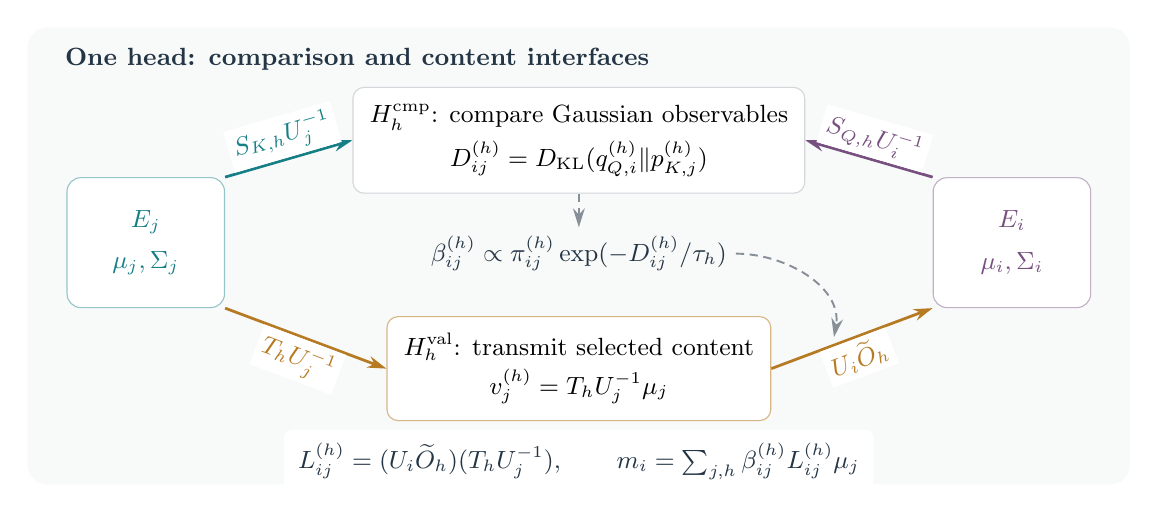
\begin{tikzpicture}[
  >={Stealth[length=2.4mm,width=1.5mm]},
  every node/.style={font=\small},
  paneltitle/.style={font=\small\bfseries,text=ink,anchor=west},
  port/.style={rounded corners=5pt,draw=ink!20,fill=white,minimum width=2.0cm,minimum height=1.65cm,align=center,inner sep=8pt},
  channel/.style={rounded corners=4pt,draw=ink!20,fill=white,minimum width=4.3cm,minimum height=1.0cm,align=center,inner sep=6pt},
  map/.style={->,line width=1.0pt},
  maplabel/.style={font=\small,fill=white,inner sep=2pt},
  control/.style={->,densely dashed,draw=ink!55,line width=.7pt}
]
\definecolor{ink}{HTML}{243545}
\definecolor{sender}{HTML}{167F86}
\definecolor{receiver}{HTML}{775080}
\definecolor{linkgold}{HTML}{B67A23}
\definecolor{paperblue}{HTML}{F1F6F8}

\fill[ink!3,rounded corners=7pt] (0,-.72) rectangle (14,5.08);
\node[paneltitle] at (.35,4.68) {One head: comparison and content interfaces};

\node[port,draw=sender!45,text=sender] (source) at (1.50,2.35)
  {\(E_j\)\\[4pt]\(\mu_j,\Sigma_j\)};
\node[port,draw=receiver!45,text=receiver] (target) at (12.50,2.35)
  {\(E_i\)\\[4pt]\(\mu_i,\Sigma_i\)};
\node[channel] (cmp) at (7.0,3.65)
  {\(H_h^{\mathrm{cmp}}\): compare Gaussian observables\\[3pt]
   \(D_{ij}^{(h)}=D_{\mathrm{KL}}(q_{Q,i}^{(h)}\|p_{K,j}^{(h)})\)};
\node[channel,draw=linkgold!55] (val) at (7.0,.75)
  {\(H_h^{\mathrm{val}}\): transmit selected content\\[3pt]
   \(v_j^{(h)}=T_hU_j^{-1}\mu_j\)};

\draw[map,sender] (source.north east) -- node[maplabel,above,sloped] {\(S_{K,h}U_j^{-1}\)} (cmp.west);
\draw[map,receiver] (target.north west) -- node[maplabel,above,sloped] {\(S_{Q,h}U_i^{-1}\)} (cmp.east);
\draw[map,linkgold] (source.south east) -- node[maplabel,below,sloped] {\(T_hU_j^{-1}\)} (val.west);
\draw[map,linkgold] (val.east) -- node[maplabel,below,sloped] {\(U_i\widetilde O_h\)} (target.south west);
\node[font=\small,text=ink,fill=ink!3,inner sep=3pt] (route) at (7.0,2.21)
  {\(\beta_{ij}^{(h)}\propto\pi_{ij}^{(h)}\exp(-D_{ij}^{(h)}/\tau_h)\)};
\draw[control] (cmp.south) -- (route.north);
\draw[control] (route.east) to[out=0,in=80] (10.24,1.15);
\node[font=\small,text=ink,fill=white,rounded corners=3pt,inner sep=5pt] at (7.0,-.43)
  {\(L_{ij}^{(h)}=(U_i\widetilde O_h)(T_hU_j^{-1}),\qquad
     m_i=\sum_{j,h}\beta_{ij}^{(h)}L_{ij}^{(h)}\mu_j\)};
\end{tikzpicture}
}
\caption{\textbf{Separate comparison and content interfaces.}
Query and key maps send Gaussian observables into a common comparison space, where their divergence determines the routing weight. The content maps \(T_hU_j^{-1}\) and \(U_i\widetilde O_h\) extract and place the transmitted mean. Their composition is the matrix link \(L_{ij}^{(h)}\); dashed arrows show scalar routing control, not an additional state map. The Gibbs weights are derived in Section~\ref{sec:mixture_derivation}.}
\label{fig:comparison_content_interfaces}
\end{figure}

\subsection{Depth, token priors, and prediction}
\label{sec:depth_prediction}

At depth \(\ell\), choose comparison and content maps \(S_Q^{(\ell)},S_K^{(\ell)},T^{(\ell)},O^{(\ell)}\). The frame field may be shared across depths while the communication maps vary. An attention residual can be followed by an affine normalization and a coordinate residual MLP. One such composition is
\begin{align}
u_i^{(\ell)}&=\operatorname{LayerNorm}_{\gamma,b}
 \bigl(\mu_i^{\mathrm{att},(\ell)}\bigr),\\
\mu_i^{(\ell+1)}&=u_i^{(\ell)}
+W_2^{(\ell)}\operatorname{GELU}\bigl(W_1^{(\ell)}u_i^{(\ell)}+b_1^{(\ell)}\bigr)
+b_2^{(\ell)}.
\label{eq:relational_block_composition}
\end{align}
Here the parameters \(\gamma,b\) of the layer normalization \citep{ba2016layernorm} are shared across depths, the MLP parameters may differ, and \(\operatorname{GELU}\) is the Gaussian error linear unit \citep{hendrycks2016gaussian}. Two covariance contracts are considered. Covariance passthrough, \(\Sigma_i^{(\ell+1)}=\Sigma_i^{(\ell)}\), defines covariance as a routing state rather than the propagated uncertainty of the nonlinear mean map; it remains an input to subsequent comparisons. Moment matching instead returns from attention the covariance of the declared predictive kernel of Theorem~\ref{thm:probabilistic_status}, which depends on the context through the routing and the source moments, and passes it through the normalization and MLP. Neither contract propagates uncertainty through the nonlinear block. This construction specifies a predictive architecture; it does not identify the normalized mean with a draw from a transformed Gaussian law.

A coordinatewise activation and fixed affine normalization do not in general commute with arbitrary \(\mathrm{GL}(K)\) transformations. Consequently, the covariance of Theorem~\ref{thm:reference_moments} does not extend automatically to this whole block. Corollary~\ref{cor:normal_form} gives the normal form of the evaluated block and its covariant alternatives, and Appendix~\ref{sec:nonlinear_gaussian_scope} makes the Gaussian-closure restriction explicit.


\label{sec:embeddings}

In standard transformers, token embeddings map discrete tokens to continuous vectors via a learned embedding matrix $W_{\text{embed}}\in\mathbb{R}^{V\times K}$. In the present construction, each token type $c \in \{1, \ldots, V\}$ is associated with a learned prior distribution:
\begin{equation}
p_c = \mathcal{N}(\mu_p^c, \Sigma_p^c), \qquad \phi_c \in \mathfrak{gl}(K),
\label{eq:prior_bank}
\end{equation}
comprising a prior mean $\mu_p^c$, prior covariance $\Sigma_p^c$, and gauge frame coefficients $\phi_c$. At the start of each sequence, agent $i$'s belief is initialized to the prior of its token type: $q_i(0) = p_{\mathrm{token}(i)}$. The collection $\{(\mu_p^c, \Sigma_p^c, \phi_c)\}_{c=1}^V$ constitutes a prior bank: a Gaussian embedding table in the sense of \citet{Vilnis2015Gaussian}, extended by frame coefficients. If only the means are retained, their table $W_{\mathrm{embed}}=[\mu_p^1,\ldots,\mu_p^V]^\top$ has the role of an ordinary embedding matrix. Isotropy alone does not remove the covariance or frame parameters.


The bank initializes the input state independently of the choice of output decoder. Positional frame factors can be composed with its token frame before communication. Using Gaussian templates to encode a token therefore does not require the optional Gaussian-bank vocabulary readout of Appendix~\ref{sec:prior_bank_readout}.

\label{sec:autoregressive_prediction}

For input positions \(x_0,\ldots,x_{N-1}\), causal source support is \(S_i=\{0,\ldots,i\}\). The sequence model has the normalized factorization
\begin{equation}
p_\theta(x_0,\ldots,x_N)
=p_\theta(x_0)\prod_{i=0}^{N-1}p_\theta(x_{i+1}\mid x_{\le i}).
\label{eq:next_token_factorization_v2}
\end{equation}
A proper initial-token law completes the joint. A linear categorical decoder specifies the next-token factors from the final mean,
\begin{equation}
p_\theta(x_{i+1}=v\mid x_{\le i})
=\operatorname{softmax}_v\left(
W_{\mathrm{out}}\mu_i^{(L)}+b_{\mathrm{out}}
+\kappa_{\mathrm{uni}}\log p_{\mathrm{uni}}\right),
\label{eq:predictive_linear_decoder}
\end{equation}
where \(p_{\mathrm{uni}}\) is a positive vocabulary prior. This decoder is itself a Gibbs readout of shared-covariance templates (Section~\ref{sec:content_laws}), and the token-bank decoder of Appendix~\ref{sec:prior_bank_readout} is another choice. Minimizing next-token cross-entropy trains this composed conditional predictor through all of its differentiable components. The observed next token supplies the training target; it is not an input to the causal state construction. Algorithm~\ref{alg:predictive_content_current} gives the evaluated realization in the experimental methods. In that evaluation each conditional is computed from a window of at most 128 tokens with stride 32; replacing \(x_{\le i}\) by that window leaves every factor normalized, so the reported perplexity is the log-loss of the resulting sequence law.

\section{Lie-Algebra Links}
\label{sec:lie_links}

The content link of Eq.~\eqref{eq:main_content_link} is a composite of site frames and shared maps, and a single head of width $s_h<K$ makes it singular. A lattice link variable is instead a group element attached to an edge, and the algebra-valued potential is its logarithmic coordinate \citep{WilsonConfinement1974,Creutz1983}. This section takes the group-valued link as the primary communication object, writes it through a generator in the Lie algebra $\mathfrak{gl}(K,\mathbb R)$, and derives the selective content maps of Section~\ref{sec:attention_operator} from that generator. Exponentiation fixes the group domain and the endpoint law. It does not select the generator, the aggregation over sources, or the residual, and each of these is stated below as a separate modeling choice.

\subsection{Exponential links and their endpoint law}
\label{sec:lie_definition}

\begin{definition}[Lie-algebra link]
\label{def:lie_link}
For a generator $X_{ij}\in\mathfrak{gl}(K,\mathbb R)$ expressed in reference coordinates, the Lie-algebra link, or exponential link, from source $j$ to receiver $i$ is
\begin{equation}
\Theta_{ij}=U_i\exp(X_{ij})U_j^{-1}:E_j\longrightarrow E_i,
\label{eq:lie_link}
\end{equation}
and its reference representative is $U_i^{-1}\Theta_{ij}U_j=\exp(X_{ij})$.
\end{definition}

\begin{proposition}[Endpoint law and invertibility]
\label{prop:lie_endpoint}
Let $X_{ij}\in\mathfrak{gl}(K,\mathbb R)$.
\begin{enumerate}
\item Under the passive site action of Eq.~\eqref{eq:passive_site_action}, with the reference generator held fixed, $\Theta_{ij}'=g_i\Theta_{ij}g_j^{-1}$.
\item Under the common reference change $U_i\mapsto U_ia$, the same local link is represented by the generator $a^{-1}X_{ij}a$, the adjoint action of $\mathrm{GL}(K)$ on its Lie algebra.
\item $\det\Theta_{ij}=\det(U_iU_j^{-1})e^{\operatorname{tr}X_{ij}}\ne0$. Every exponential link is invertible, including links with singular generators, and $\Theta_{ij}^{-1}=U_je^{-X_{ij}}U_i^{-1}$.
\item A matrix $G\in\mathrm{GL}(K,\mathbb R)$ equals $e^X$ for some real $X$ exactly when, for each negative eigenvalue of $G$ and each block size, the Jordan blocks of that eigenvalue and size occur an even number of times. Every such $G$ lies in the identity component $\mathrm{GL}^+(K)$, and for $K\ge2$ not every element of $\mathrm{GL}^+(K)$ is of this form.
\end{enumerate}
\end{proposition}
\begin{proof}
Item 1 follows by substituting $U_i'=g_iU_i$ into Eq.~\eqref{eq:lie_link}. Item 2 follows from $\exp(a^{-1}Xa)=a^{-1}\exp(X)a$, which holds term by term in the exponential series, so that $(U_ia)\exp(a^{-1}X_{ij}a)(U_ja)^{-1}=\Theta_{ij}$. Item 3 is the identity $\det e^X=e^{\operatorname{tr}X}$ \citep{Hall2015}. The characterization in item 4 is Theorem~1 of \citet{culver1966existence}, and membership in $\mathrm{GL}^+(K)$ follows from item 3. For the last statement, $\operatorname{diag}(-1,-2)\oplus I_{K-2}$ has positive determinant and two negative eigenvalues, each with a single Jordan block of size one, so it has no real logarithm.
\end{proof}

The generator is reference data. The frames carry the entire passive action, as they do for the comparison and content maps of Section~\ref{sec:role_measurements}, and $X_{ij}$ changes only under a common change of the reference basis. In lattice gauge theory the link $e^{aA}$ has the algebra-valued potential $A$ as its logarithmic coordinate, and $A$ transforms as a connection under local gauge transformations \citep{Creutz1983}. Here the frames dress the potential, so the generator is invariant under independent site changes of frame, while the link $\Theta_{ij}$ transforms exactly as a lattice link variable. When the reference representative has no eigenvalue on the closed negative real axis, it has a unique real logarithm whose eigenvalues lie in the strip $|\operatorname{Im}z|<\pi$, the principal logarithm \citep[Thm.~1.31]{Higham2008}. The principal logarithm is therefore a chart on the open subset of $\mathrm{GL}^+(K)$ without eigenvalues on the closed negative real axis; it is not a global chart of the group.

\subsection{Why the links are group valued}
\label{sec:lie_motivation}

Four structural facts motivate placing the link in the group rather than in the space of all matrices. The first concerns rank. A single head with $s_h<K$ gives $\operatorname{rank}L_{ij}^{(h)}\le s_h$, so for every matrix $N$ the product $L_{ij}^{(h)}N$ is singular, and no group element factors as $L_{ij}^{(h)}N$ through a selective channel. The relation between a selective channel and an invertible link must therefore be additive, through a block, or infinitesimal through the Lie algebra, and the construction of Section~\ref{sec:lie_lowrank} realizes all three.

The second concerns loops. On the causal support every closed directed walk is a self-loop (Theorem~\ref{thm:reference_moments}), so routed products of causal links contain no loop through distinct positions. An invertible link supplies the reverse edge $\Theta_{ij}^{-1}$ without new parameters, and inverse-edge triangles then carry conjugation-invariant holonomies on the causal graph (Section~\ref{sec:lie_holonomy}). A singular link admits closed matrix products only on a separately declared extended graph.

The third concerns the singular boundary. An additive update of an invertible matrix $M$ can reach the singular set in a single step of spectral norm $\sigma_{\min}(M)$: for unit singular vectors $u,v$ belonging to $\sigma_{\min}(M)$, the matrix $M-\sigma_{\min}(M)uv^\top$ annihilates $v$. The exponential parametrization keeps $\det e^X=e^{\operatorname{tr}X}>0$ for every finite generator, and $\sigma_{\min}(e^X)\ge e^{-\|X\|_2}$ because $\|e^{-X}\|_2\le e^{\|X\|_2}$. For an exact Gaussian pushforward, the singular boundary also lies at infinite statistical distance.

\begin{proposition}[The singular boundary is at infinite distance]
\label{prop:lie_boundary}
Let $q_0=\mathcal N(\mu_0,\Sigma_0)$ with $\Sigma_0\succ0$, let $g\in\mathrm{GL}(K)$, and let $q_g=\mathcal N(g\mu_0,g\Sigma_0g^\top)$. If $\lambda_{\min}$ is the smallest eigenvalue of $\Sigma_0^{-1/2}g\Sigma_0g^\top\Sigma_0^{-1/2}$, then
\begin{equation}
d_{\mathrm{FR}}(q_0,q_g)\ge\tfrac{1}{\sqrt2}\bigl|\log\lambda_{\min}\bigr|.
\label{eq:lie_fr_bound}
\end{equation}
As $g$ approaches a singular matrix, $\lambda_{\min}\to0$ and the Fisher--Rao distance diverges.
\end{proposition}
\begin{proof}
Let $w=\Sigma_0^{-1/2}e$ for a unit eigenvector $e$ belonging to $\lambda_{\min}$. The scalar observable $w^\top x$ has variance $w^\top\Sigma_0w=1$ under $q_0$ and $w^\top g\Sigma_0g^\top w=\lambda_{\min}$ under $q_g$. The univariate Gaussian family with mean $m$ and standard deviation $s$ has Fisher metric $(dm^2+2ds^2)/s^2$, so every path between standard deviations $1$ and $\lambda_{\min}^{1/2}$ has length at least $\sqrt2|\log\lambda_{\min}^{1/2}|$. Marginalization to $w^\top x$ is a Markov morphism and does not increase Fisher--Rao length \citep{AmariNagaoka2000}, which gives Eq.~\eqref{eq:lie_fr_bound}. If $g$ tends to a singular matrix $g_\star$, then $g_\star\Sigma_0g_\star^\top$ is singular, and continuity of eigenvalues gives $\lambda_{\min}\to0$.
\end{proof}

The proposition concerns the exact pushforward of a fixed nondegenerate Gaussian. A positive covariance floor or additive receiving noise changes this geometry, so it is not a claim that a training objective diverges when a content map becomes singular. The fourth fact is that the generator is a linear coordinate on which a Gaussian prior, a natural gradient, and latent inference can be written, and Section~\ref{sec:latent_links} uses it in this way.

\subsection{Low-rank generators and the selective channels}
\label{sec:lie_lowrank}

The generator whose first-order term reproduces the content link is built from the stored value and output maps. Its exponential has an exact closed form through the entire function
\begin{equation}
\varphi_1(Z)=\sum_{n\ge1}\frac{Z^{n-1}}{n!},\qquad \varphi_1(Z)=(e^Z-I)Z^{-1}\ \text{for invertible}\ Z,
\label{eq:lie_phi1}
\end{equation}
the first of the $\varphi$-functions of exponential integrators \citep{Hochbruck2010}.

\begin{lemma}[Exponential of a low-rank generator]
\label{lem:lie_lowrank}
For $P\in\mathbb R^{K\times s}$ and $Q\in\mathbb R^{s\times K}$,
\begin{equation}
\exp(PQ)=I_K+P\varphi_1(QP)Q.
\label{eq:lie_lowrank}
\end{equation}
\end{lemma}
\begin{proof}
For $n\ge1$, regrouping the product gives $(PQ)^n=P(QP)^{n-1}Q$. Summing the exponential series term by term gives $I_K+P\bigl(\sum_{n\ge1}(QP)^{n-1}/n!\bigr)Q$, and the inner series converges for every $s\times s$ matrix.
\end{proof}

\begin{proposition}[Flat transport plus a channel term]
\label{prop:lie_split}
For one head with stored maps $T_h,O_h$ and the generator $X_{ij}=O_hT_h$,
\begin{equation}
\Theta_{ij}=\Omega_{ij}+U_iO_h\varphi_1(T_hO_h)T_hU_j^{-1}.
\label{eq:lie_split}
\end{equation}
\begin{enumerate}
\item $\exp(O_hT_h)$ acts as the identity on $\ker T_h$, so on the subspace $U_j\ker T_h$ that the head does not read, $\Theta_{ij}$ coincides with the flat identification $\Omega_{ij}$.
\item The image of $\exp(O_hT_h)-I$ lies in $\operatorname{im}O_h$, so $\Theta_{ij}$ differs from $\Omega_{ij}$ only in directions that the head writes.
\item For $X_{ij}=sO_hT_h$, $\Theta_{ij}=\Omega_{ij}+sU_iO_hT_hU_j^{-1}+O(s^2)$, so the projected matrix link is the first-order channel.
\item $\det\Theta_{ij}=\det(U_iU_j^{-1})e^{\operatorname{tr}(T_hO_h)}$.
\end{enumerate}
The same statements hold for the stacked generator $X=OT=\sum_hO_hT_h$, with $O=[O_1\ \cdots\ O_H]\in\mathbb R^{K\times S}$, $T=[T_1;\cdots;T_H]\in\mathbb R^{S\times K}$, and $S=\sum_hs_h$.
\end{proposition}
\begin{proof}
Equation~\eqref{eq:lie_split} is Lemma~\ref{lem:lie_lowrank} with $P=O_h$ and $Q=T_h$, conjugated by the frames. Items 1 and 2 are read off from the correction term, which has the form $O_h(\cdots)T_h$. Item 3 follows from $\varphi_1(sZ)=I+O(s)$, and item 4 from $\det e^X=e^{\operatorname{tr}X}$ with $\operatorname{tr}(O_hT_h)=\operatorname{tr}(T_hO_h)$.
\end{proof}

Every entry of $\Theta_{ij}$ is determined by the frames and the stored maps. The link is the identity transport on the unread complement and carries the channel term, which equals the projected matrix link to first order and acquires the corrections $\varphi_1(T_hO_h)$ at higher order. Contracting the scaled link $\Theta_{ij}(s)=U_ie^{sO_hT_h}U_j^{-1}$ against one routing row at fixed source states gives
\begin{equation}
\sum_j\beta_{ij}\Theta_{ij}(s)\mu_j
=\sum_j\beta_{ij}\Omega_{ij}\mu_j
+s\sum_j\beta_{ij}U_iO_hT_hU_j^{-1}\mu_j+O(s^2).
\label{eq:lie_two_orders}
\end{equation}
The zeroth-order term transports complete source states by the flat identification, which is the message of complete-state alignment (Section~\ref{sec:mixture_derivation}), and the first-order term is the projected predictive message of Eq.~\eqref{eq:relational_predictive_residual} in the affine chart. Both message forms are thus orders of one exponential link. This is a statement about the form of the message; it does not recover either objective. With an independent source label for each head, the zeroth-order term becomes a head-routed flat transport (Proposition~\ref{prop:lie_order_zero}).

\subsection{Linear and exponential links as charts of one group}
\label{sec:lie_charts}

The phrase ``first-order channel'' could suggest that the matrix link is a weak-field truncation of the exponential link. On a specified logarithm domain the relation is instead an exact change of coordinates. Fix $O\in\mathbb R^{K\times s}$ and $T\in\mathbb R^{s\times K}$ with $TO$ invertible, so that $\mathbb R^K=W\oplus W'$ with $W=\operatorname{im}O$ and $W'=\ker T$, and let $\Pi=O(TO)^{-1}T$ be the projector onto $W$ along $W'$. For $B\in\mathrm{GL}(s)$ put
\begin{equation}
\Upsilon(B)=(I-\Pi)+OB(TO)^{-1}T,
\label{eq:lie_embed}
\end{equation}
the operator that fixes $W'$ pointwise and acts on $W$ as $B$ in the basis formed by the columns of $O$.

\begin{proposition}[Two charts of one group]
\label{prop:lie_charts}
\begin{enumerate}
\item $\Upsilon:\mathrm{GL}(s)\to\mathrm{GL}(K)$ is an injective homomorphism with $\det\Upsilon(B)=\det B$. Its image is the factor of the block-diagonal Levi subgroup $\mathrm{GL}(W)\times\mathrm{GL}(W')$ that acts trivially on $W'$.
\item Linear links: for $C\in\mathbb R^{s\times s}$, $I+OCT=\Upsilon(I_s+CTO)$, so $\det(I+OCT)=\det(I_s+CTO)$.
\item Exponential links: $\exp(OT)=\Upsilon(e^{TO})$.
\item Exact conversion: let $O_{\mathrm{lin}}\in\mathbb R^{K\times s}$ be such that $I_s+TO_{\mathrm{lin}}$ has no eigenvalue on $(-\infty,0]$, put $Z=\log(I_s+TO_{\mathrm{lin}})$ with the principal logarithm, and put $O=O_{\mathrm{lin}}\varphi_1(Z)^{-1}$. Then $\varphi_1(Z)$ is invertible, $TO=Z$, and
\begin{equation}
\exp(OT)=I_K+O_{\mathrm{lin}}T.
\label{eq:lie_conversion}
\end{equation}
\end{enumerate}
\end{proposition}
\begin{proof}
For item 1, $\Upsilon(B)Oy=OBy$ because $(I-\Pi)O=0$ and $(TO)^{-1}TO=I$, and $\Upsilon(B)w'=w'$ for $w'\in W'$ because $\Pi w'=0$. An operator on $W\oplus W'$ is determined by its action on the two summands, so $\Upsilon(B)\Upsilon(B')=\Upsilon(BB')$, $\det\Upsilon(B)=\det B$, and $\Upsilon(B)=I$ only for $B=I$. For item 2, $(I+OCT)Oy=O(I+CTO)y$ and $(I+OCT)w'=w'$. For item 3, $(OT)^nO=O(TO)^n$ gives $\exp(OT)Oy=Oe^{TO}y$, and $\exp(OT)w'=w'$. For item 4, the eigenvalues of $Z$ have imaginary parts in $(-\pi,\pi)$, while the eigenvalues $(e^z-1)/z$ of $\varphi_1(Z)$ vanish only at $z\in2\pi i\mathbb Z\setminus\{0\}$, so $\varphi_1(Z)$ is invertible. Since $TO_{\mathrm{lin}}=e^Z-I=Z\varphi_1(Z)$, with $Z$ and $\varphi_1(Z)$ commuting, $TO=TO_{\mathrm{lin}}\varphi_1(Z)^{-1}=Z$. Lemma~\ref{lem:lie_lowrank} then gives $\exp(OT)=I+O\varphi_1(TO)T=I+O_{\mathrm{lin}}\varphi_1(Z)^{-1}\varphi_1(Z)T=I+O_{\mathrm{lin}}T$.
\end{proof}

Item 4 says that the flat identification plus a linear channel term, $\Omega_{ij}+U_iO_{\mathrm{lin}}TU_j^{-1}$, is exactly an exponential link for every $O_{\mathrm{lin}}$ in an open set containing $O_{\mathrm{lin}}=0$. On their common domain the linear and logarithmic parametrizations describe the same group elements, related by $I_s+TO_{\mathrm{lin}}=e^{TO}$, and the expansion of Proposition~\ref{prop:lie_split} states that the two charts agree to first order at the identity. Using one numerical generator in both $I+X$ and $e^X$ is a first-order approximation only. The choice of chart changes four things. First, the linear parameter space contains the singular matrices, and a step in $(O_{\mathrm{lin}},T)$ can carry $\det(I_K+O_{\mathrm{lin}}T)=\det(I_s+TO_{\mathrm{lin}})$ through zero, whereas the logarithmic chart cannot reach that boundary; by Proposition~\ref{prop:lie_endpoint} it also excludes the matrices without a real logarithm, including every matrix of negative determinant. Second, the two charts carry different optimization geometries, since an optimizer acting on the factors induces different changes of the composite matrix in each. Third, they differ at order one for finite generators: at $X=I$, $e^X=eI$ while $I+X=2I$. Fourth, these statements concern an unrouted operator with one generator; routed head sums and edge-dependent generators may leave the one-generator family. When the heads tile the state, $O_{\mathrm{lin}}$ is the stored factor of the first-order chart of Section~\ref{sec:lie_orders}, whose effective receiving map is $T^{-1}+O_{\mathrm{lin}}$.

\subsection{Routing outside the exponent: aggregation and the residual}
\label{sec:lie_aggregation}

The group law does not choose an aggregation over sources. A link acts on one source state, whereas a predictive mixture also needs a normalized law over source choices. Placing the routing matrix inside the exponent, $X_{ij}=O\boldsymbol\beta_{ij}T$, changes the single-edge operator and leaves the aggregation over $j$ unspecified, since neither the sum nor the product of the routed exponentials specifies how source vectors are selected. The construction below keeps categorical routing outside the exponent and uses the routing-independent stacked generator $X=OT$, so that $\beta_{ij}^{(h)}$ retains its meaning as the probability that head $h$ selects source $j$ (Theorem~\ref{thm:probabilistic_status}). It assumes that the stacked transfer $TO\in\mathbb R^{S\times S}$ is invertible, which allows $S\le K$.

\begin{lemma}[Complement split]
\label{lem:lie_complement}
With $\Pi=O(TO)^{-1}T$,
\begin{equation}
\exp(OT)=(I-\Pi)+Oe^{TO}(TO)^{-1}T.
\label{eq:lie_complement}
\end{equation}
\end{lemma}
\begin{proof}
By Lemma~\ref{lem:lie_lowrank}, $\exp(OT)=I+O\varphi_1(TO)T=(I-\Pi)+O[(TO)^{-1}+\varphi_1(TO)]T$, and $(TO)^{-1}+\varphi_1(TO)=(TO)^{-1}+(e^{TO}-I)(TO)^{-1}=e^{TO}(TO)^{-1}$ because every term is a function of $TO$.
\end{proof}

The first term is the identity on the unread complement $\ker T$ and annihilates $\operatorname{im}O$. The second reads the $S$ sent coordinates $T\xi$, mixes them through the $S\times S$ matrix $e^{TO}(TO)^{-1}$, and writes them into $\operatorname{im}O$. Write $\widetilde O=Oe^{TO}(TO)^{-1}$, and let $\widetilde O_h$ be its block column receiving head $h$. Following the predictive kernel of Theorem~\ref{thm:probabilistic_status}, each head draws its own source label $J^h$ with probability $\beta_{ij}^{(h)}$, independently across heads, and the sent block $T_h\xi$ is read from the source selected by its head. The complement term needs a carrier of its own, a label $J^0$. The transported reference state and its expectation over the independent labels are
\begin{align}
\xi_i'&=(I-\Pi)\xi_{J^0}+\sum_h\widetilde O_hT_h\xi_{J^h},
\label{eq:lie_transported_state}\\
\mathbb E[\xi_i']&=\mathbb E[(I-\Pi)\xi_{J^0}]+\sum_h\sum_j\beta_{ij}^{(h)}\widetilde O_hT_h\xi_j.
\label{eq:lie_aggregate}
\end{align}
Each sent block travels with the label of its own head, so the cross-head mixing in $e^{TO}(TO)^{-1}$ does not couple the head routings. The weights depend on the states through the comparison costs, but they are evaluated at the layer's input states and held fixed while the message is formed, so Eq.~\eqref{eq:lie_aggregate} is the expectation conditional on those states.

\begin{proposition}[Complement persistence]
\label{prop:lie_complement_persistence}
Assume that only sent content may cross between agents and that the update retains one unchanged complement taken from an existing agent state, as in Eq.~\eqref{eq:lie_transported_state}. Then the carrier is the receiver, $J^0=i$, and
\begin{equation}
\mu_i^+=U_i(I-\Pi)U_i^{-1}\mu_i+\sum_h\sum_j\beta_{ij}^{(h)}U_i\widetilde O_hT_hU_j^{-1}\mu_j.
\label{eq:lie_self_complement}
\end{equation}
\end{proposition}
\begin{proof}
The complement $\ker T$ holds exactly the directions that no head sends. A carrier $J^0=j\ne i$ would place unsent coordinates of agent $j$ in the state of agent $i$, contradicting the premise, so the receiver is the only admissible carrier within the declared unchanged-complement rule. Without that rule, locality would also permit discarding the complement or applying a receiver-local map, so locality alone does not force persistence. Equation~\eqref{eq:lie_aggregate} with $J^0=i$, conjugated by the frames, gives Eq.~\eqref{eq:lie_self_complement}.
\end{proof}

\begin{corollary}[Tiled heads leave no residual]
\label{cor:lie_tiled}
If the heads tile the reference space, $S=K$ with $O$ and $T$ invertible, then $\Pi=I$, the complement is empty, $\widetilde O=e^{OT}T^{-1}$, and
\begin{equation}
\mu_i^+=\sum_jU_i\widetilde O\boldsymbol\beta_{ij}TU_j^{-1}\mu_j
=\sum_h\sum_j\beta_{ij}^{(h)}U_i\widetilde O_hT_hU_j^{-1}\mu_j.
\label{eq:lie_tiled}
\end{equation}
\end{corollary}
\begin{proof}
With $O$ and $T$ invertible, $\Pi=OO^{-1}T^{-1}T=I$, and $O(TO)^nO^{-1}=(OT)^n$ gives $Oe^{TO}(TO)^{-1}=Oe^{TO}O^{-1}T^{-1}=e^{OT}T^{-1}$. Block multiplication gives $\sum_h\beta_{ij}^{(h)}\widetilde O_hT_h=\widetilde O\boldsymbol\beta_{ij}T$.
\end{proof}

Under complement-preserving aggregation, the receiver therefore keeps its own state exactly on the directions that no head writes and takes the transported message on the directions that heads write. That projected residual $U_i(I-\Pi)U_i^{-1}\mu_i$ differs from the full residual $r\mu_i$ of Eq.~\eqref{eq:relational_predictive_residual}. When the heads tile the state, as in the implementation, the complement is empty, so the residual $r=1$ has no counterpart in this aggregation, and the receiver's own state enters only through the self-weights $\beta_{ii}^{(h)}$. A residual of the projected kind requires channels that do not tile, $S<K$; the $K-S$ coordinates that no head reads or writes then form the residual stream. Gaussian fusion reaches a related structure by a different argument: the channel-likelihood receiver of Section~\ref{sec:receiver_inference} keeps its prior on the directions that no head observes and blends prior and message on the observed directions with a precision-weighted gain (Eq.~\eqref{eq:rec_fusion_residual}). The additive residual $\mu_i+m_i$ is neither. It is the residual connection of residual networks \citep{He2016ResNet}, added in every direction without normalization.

\subsection{The tiled message order by order}
\label{sec:lie_orders}

In the setting of Corollary~\ref{cor:lie_tiled}, with tiled heads, square invertible stacked maps, the shared generator $X=OT$, and routing outside the exponent, the receiving maps sum in closed form, and expanding them in the scale of the generator separates the message into orders with distinct roles. Write $\xi_j=U_j^{-1}\mu_j$ for the reference source states.

\begin{proposition}[Resummed receiving map]
\label{prop:lie_resummed}
Under these assumptions,
\begin{equation}
\widetilde O=e^{OT}T^{-1}=T^{-1}+O\varphi_1(TO),\qquad
\mu_i^+=U_i\sum_j\widetilde O\boldsymbol\beta_{ij}T\xi_j.
\label{eq:lie_resummed}
\end{equation}
The effective transfer is $T\widetilde O=e^{TO}$, so $\det(T\widetilde O)=e^{\operatorname{tr}(TO)}>0$.
\end{proposition}
\begin{proof}
The first form is Corollary~\ref{cor:lie_tiled}. Lemma~\ref{lem:lie_lowrank} gives $e^{OT}=I+O\varphi_1(TO)T$, and multiplying on the right by $T^{-1}$ gives the second form. Finally $T\widetilde O=Te^{OT}T^{-1}=e^{TO}$, and $\det e^{Z}=e^{\operatorname{tr}Z}$.
\end{proof}

Replacing $O$ by $sO$ at fixed $T$, so that $X=sOT$, gives the series
\begin{equation}
\widetilde O(s)=T^{-1}+sO\varphi_1(sTO)=T^{-1}+\sum_{n\ge1}\frac{s^n}{n!}O(TO)^{n-1},
\label{eq:lie_orders}
\end{equation}
which converges for every $s$. The order-$n$ message replaces $\widetilde O$ in Eq.~\eqref{eq:lie_resummed} by its order-$n$ term at $s=1$.

\begin{proposition}[Zeroth order]
\label{prop:lie_order_zero}
Let $\Delta_h$ be the coordinate projector onto the head-$h$ block of $\mathbb R^S$, and let $\Pi_h=T^{-1}\Delta_hT$. Then $\Pi_h=(T^{-1})_{:,h}T_h$, $\Pi_h\Pi_g=\delta_{hg}\Pi_h$, $\sum_h\Pi_h=I_K$, $\ker\Pi_h=\ker T_h$, $\operatorname{im}\Pi_h=\bigcap_{g\ne h}\ker T_g$, and
\begin{equation}
T^{-1}\boldsymbol\beta_{ij}T=\sum_h\beta_{ij}^{(h)}\Pi_h.
\label{eq:lie_order_zero}
\end{equation}
If every head uses the same routing, $\beta_{ij}^{(h)}=\beta_{ij}$, as always holds for $H=1$, the zeroth-order message is $\sum_j\beta_{ij}\Omega_{ij}\mu_j$.
\end{proposition}
\begin{proof}
The relations $\Delta_h\Delta_g=\delta_{hg}\Delta_h$ and $\sum_h\Delta_h=I$ survive conjugation by $T$, and Eq.~\eqref{eq:lie_order_zero} is $\boldsymbol\beta_{ij}=\sum_h\beta_{ij}^{(h)}\Delta_h$ conjugated by $T$. Writing $T^{-1}$ by block columns gives $\Pi_h=(T^{-1})_{:,h}T_h$. Since $\Delta_hTx$ has the single nonzero block $T_hx$, $\Pi_hx=0$ exactly when $T_hx=0$, and $x\in\operatorname{im}\Pi_h=T^{-1}\operatorname{im}\Delta_h$ exactly when $T_gx=0$ for every $g\ne h$. A shared routing has $\boldsymbol\beta_{ij}=\beta_{ij}I$, so $U_iT^{-1}\boldsymbol\beta_{ij}T\xi_j=\beta_{ij}\Omega_{ij}\mu_j$.
\end{proof}

The zeroth-order message $U_i\sum_h\sum_j\beta_{ij}^{(h)}\Pi_h\xi_j$ is a head-routed flat transport. Head $h$ carries, unmixed and routed by its own weights, the component $\Pi_h\xi_j$ of each source state in the directions that no other head reads. The projectors are oblique in general, and the sum includes the receiver through $\beta_{ii}^{(h)}$, so this term is not the residual $r\mu_i$. The first-order term $U_i\sum_jO\boldsymbol\beta_{ij}T\xi_j$ is the standard multi-head value path with value maps $T_h$ and output maps $O_h$ (Section~\ref{sec:value_aggregation}). The second-order term,
\begin{equation}
\tfrac12O(TO)\boldsymbol\beta_{ij}T=\tfrac12\sum_{g,h}O_g(T_gO_h)\beta_{ij}^{(h)}T_h,
\label{eq:lie_order_two}
\end{equation}
is cross-head mixing. The routed block of head $h$ is written by $O_h$, read again by every head $g$ through the block $T_gO_h$ of the head-transfer matrix $TO$, and rewritten by $O_g$, with the same source and no second routing. The order-$n$ term makes $n-1$ such round trips with weight $1/n!$.

The orders do not enlarge the family of mean maps. For invertible $T$ the map $O\mapsto T^{-1}+O$ is a bijection, so the first-order truncation reaches every receiving map, as the affine chart does. Since $OT$ ranges over all of $\mathfrak{gl}(K)$, the exponential chart reaches a receiving map $\widetilde O$ exactly when $\widetilde OT$ has a real logarithm $X$, with $O=XT^{-1}$, and by Proposition~\ref{prop:lie_endpoint} this forces $\det(\widetilde OT)>0$. The three parametrizations therefore represent the same tiled shared-generator mean maps up to the real-logarithm domain. They differ in what the zero of the stored factor means, in the reachable component, and in the conditioning and optimization geometry of the trained links, and these are the properties that a comparison between them tests.

A finite truncation is a separate model that approximates the exponential only for small generators. Truncation after order $n$ gives $\widetilde O_nT=p_n(X)$ with $p_n(z)=\sum_{k\le n}z^k/k!$, and the remainder obeys $\|e^X-p_n(X)\|_2\le\sum_{k>n}\|X\|_2^k/k!$, which is small only when $\|X\|_2$ is small compared with $n$. No finite truncation is structurally group valued. Every $p_n$ with $n\ge1$ has a complex root, which is an eigenvalue of some real $Z$ when $K\ge2$, through a rotation-scaling block if it is not real, and $p_n(Z)$ is then singular by spectral mapping. For example, $I+Z+Z^2/2=\tfrac12[(Z+I)^2+I]$ vanishes at $Z=\bigl(\begin{smallmatrix}-1&-1\\1&-1\end{smallmatrix}\bigr)$. The exponential has no zeros and is therefore invertible for every generator.

The stored factors therefore admit three effective receiving maps, which define the affine, first-order, and exponential charts of the implementation:
\begin{equation}
\widetilde O=O,\qquad
\widetilde O=T^{-1}+O,\qquad
\widetilde O=T^{-1}+O\varphi_1(TO)=e^{OT}T^{-1}.
\label{eq:lie_three_charts}
\end{equation}
The affine chart keeps only the first-order channel, so $O=0$ means zero content. The first-order chart keeps orders zero and one. It has the same function class as the affine chart but is centered at the head-routed flat transport, so a decay of the stored factor pulls toward that transport rather than toward zero content. The exponential chart has the same center, differs from the first-order chart from second order in $O$ on, and is the only chart whose effective transfer stays in $\mathrm{GL}^+(K)$. At the block-projector initialization $T=I$, the content $c_{\mathrm{out}}\boldsymbol\beta_{ij}$ at output scale $c_{\mathrm{out}}>0$ requires $O=c_{\mathrm{out}}I$, $(c_{\mathrm{out}}-1)I$, and $(\log c_{\mathrm{out}})I$ in the three charts, since $z\varphi_1(z)=e^z-1$ equals $c_{\mathrm{out}}-1$ at $z=\log c_{\mathrm{out}}$. At $c_{\mathrm{out}}=1$ both centered charts start at $O=0$, whereas reusing $O=I$ in the exponential chart would start the content at $e\boldsymbol\beta_{ij}$. The factor $\varphi_1(TO)$ needs no inverse of $TO$: for every square $A$,
\begin{equation}
\exp\begin{pmatrix}A&I\\0&0\end{pmatrix}=\begin{pmatrix}e^{A}&\varphi_1(A)\\0&I\end{pmatrix},
\label{eq:lie_augmented}
\end{equation}
because $\bigl(\begin{smallmatrix}A&I\\0&0\end{smallmatrix}\bigr)^n=\bigl(\begin{smallmatrix}A^n&A^{n-1}\\0&0\end{smallmatrix}\bigr)$ for $n\ge1$. This is the two-block case of the block-triangular exponential formula of \citet{VanLoan1978}, so one exponential of size $2S$ returns $e^{TO}$ and $\varphi_1(TO)$.

A chart changes only the effective receiving map. Every statement of Sections~\ref{sec:passive_covariance} to~\ref{sec:receiver_inference} that involves the content maps uses them only through $\widetilde O_h$ and $T_h$, with $M_h=\widetilde O_hT_h$, and therefore holds in each chart. In particular, the moment-matched covariance of Theorem~\ref{thm:probabilistic_status} holds with that substitution, and the channel-likelihood receiver uses $\widetilde O_h^\top$ as its measurement.

\begin{remark}[Routed exponents and self-gates]
\label{rem:lie_routed_exponent}
The routed generator $X_{ij}=O\boldsymbol\beta_{ij}T$ gives $\exp(O\boldsymbol\beta_{ij}T)=I+O\varphi_1(\boldsymbol\beta_{ij}TO)\boldsymbol\beta_{ij}T$ by Lemma~\ref{lem:lie_lowrank}. Its first-order term is the routed head sum, and heads interact from second order on through the blocks of $TO$. Because the weights depend on the states, $\varphi_1(\boldsymbol\beta_{ij}TO)$ is then a matrix function of the states. On the self-link this is a single-source transformation and needs no aggregation rule; for tiled heads with $TO=I$ it equals $\sum_he^{\beta_{ii}^{(h)}}O_hT_h$, a gate in $(1,e]$ on each head block whose argument is the self-routing weight. A general state-dependent self-generator $X(\xi)=\operatorname{diag}(a(\xi))$ gives the coordinatewise gate $\xi_k\mapsto\xi_ke^{a_k(\xi)}$, and every positive gate has this form. The SiLU $x\operatorname{sgm}(x)$, with $\operatorname{sgm}$ the logistic function, and the GELU $x\Phi_{\mathcal N}(x)$, with $\Phi_{\mathcal N}$ the standard normal distribution function, are exponential self-links with generators $\log\operatorname{sgm}$ and $\log\Phi_{\mathcal N}$ \citep{hendrycks2016gaussian}. This rewriting places the MLP in the same group-valued language as the links, but it does not derive the generator.
\end{remark}

\section{Covariance and the Reference-Coordinate Normal Form}
\label{sec:passive_covariance}

The operator of Section~\ref{sec:attention_operator} is written with frames, but every routing cost and message it computes factors through the reference moments. This section makes that statement exact, derives its consequences, and states what it does and does not constrain.

\begin{lemma}[Invariance of divergences under invertible maps]
\label{lem:glk_invariance}
For probability laws $P$ and $Q$ on $\mathbb R^K$ with densities and any $A\in\mathrm{GL}(K)$,
\begin{equation}
D_{\mathrm{KL}}(A_*P\|A_*Q)=D_{\mathrm{KL}}(P\|Q).
\label{eq:glk_invariance}
\end{equation}
\end{lemma}
\begin{proof}
Both densities acquire the same Jacobian factor, which cancels in their ratio \citep{Amari2016}. The same argument applies to $f$-divergences, and the data-processing inequality applied to $A$ and $A^{-1}$ gives equality for every R\'enyi order \citep[Thm.~9]{vanErvenHarremoes2014}.
\end{proof}
This common invertible change of coordinates is distinct from a rank-reducing measurement or a change to the learned interfaces.

\begin{theorem}[Reference-moment factorization]
\label{thm:reference_moments}
Fix a layer, its comparison maps $S_{Q,h}$, $S_{K,h}$, its stored content maps $T_h$, $O_h$ with effective receiving maps $\widetilde O_h$ in one chart of Eq.~\eqref{eq:lie_three_charts}, its source priors, its temperatures, and its residual coefficient $r$, and write $M_h=\widetilde O_hT_h$.
\begin{enumerate}
\item Every routing cost $D_{ij}^{(h)}$ and weight $\beta_{ij}^{(h)}$ depends on the states only through the reference moments $(\xi_j,C_j)$, and $U_i^{-1}\mu_i^{\mathrm{att}}=r\xi_i+\sum_{j,h}\beta_{ij}^{(h)}M_h\xi_j$.
\item Under the passive site action of Eq.~\eqref{eq:passive_site_action}, the routing weights are unchanged, and the routed contributions $\mathcal M_{ij}^{(h)}=\beta_{ij}^{(h)}L_{ij}^{(h)}$ and messages transform as
\begin{equation}
\mathcal M_{ij}^{(h)\prime}=g_i\mathcal M_{ij}^{(h)}g_j^{-1},
\qquad m_i'=g_i m_i.
\label{eq:relational_covariance}
\end{equation}
\item The operator is unchanged by the common reference change $(U_i,S_{Q,h},S_{K,h},T_h,O_h)\mapsto(U_ia,S_{Q,h}a,S_{K,h}a,T_ha,a^{-1}O_h)$ with $a\in\mathrm{GL}(K)$, under which the stored generator transforms as $OT\mapsto a^{-1}OTa$, by $(S_{Q,h},S_{K,h})\mapsto(AS_{Q,h},AS_{K,h})$ with $A\in\mathrm{GL}(r_h)$, and by the headwise change $(T_h,O_h)\mapsto(B_hT_h,O_hB_h^{-1})$ with $B_h\in\mathrm{GL}(s_h)$, in each chart. The common reference change also leaves every operation in local coordinates unchanged.
\item For a closed walk $\gamma=(i_0,\ldots,i_r=i_0)$, the routed loop product $\mathcal H_\gamma=\mathcal M_{i_0i_1}\cdots\mathcal M_{i_{r-1}i_0}$ satisfies $\mathcal H_\gamma'=g_{i_0}\mathcal H_\gamma g_{i_0}^{-1}$, and its trace is a polynomial in the routing weights with loop-independent coefficients $\operatorname{Tr}(M_{h_1}\cdots M_{h_r})$. On the causal support $S_i=\{0,\ldots,i\}$, every closed walk is a self-loop.
\end{enumerate}
\end{theorem}
\begin{proof}
(1) The comparison laws of Eqs.~\eqref{eq:relational_query_law} and~\eqref{eq:relational_key_law} are built from $S_{Q,h}\xi_i$, $S_{Q,h}C_iS_{Q,h}^\top$, and the corresponding key moments, so the costs and the Gibbs weights of Eq.~\eqref{eq:relational_routing} depend on the states only through the reference moments. Applying $U_i^{-1}$ to Eq.~\eqref{eq:relational_predictive_residual} gives the stated reference form.
(2) Substituting the transformed variables into Eq.~\eqref{eq:overview_reference_state} gives $\xi_i'=\xi_i$ and $C_i'=C_i$, so by (1) the weights are unchanged. The content links obey Eq.~\eqref{eq:main_link_endpoint_law}, which leaves only the external factors $g_i$ and $g_j^{-1}$, and the message transforms by $g_i$.
(3) Under the common reference change, $\xi_i\mapsto a^{-1}\xi_i$ and $C_i\mapsto a^{-1}C_ia^{-\top}$, so every projected mean $S_{Q,h}\xi_i$, every projected covariance $S_{Q,h}C_iS_{Q,h}^\top$, and the corresponding key moments are unchanged. In each chart the effective receiving map transforms as $\widetilde O\mapsto a^{-1}\widetilde O$: trivially in the affine chart, as $(Ta)^{-1}+a^{-1}O=a^{-1}(T^{-1}+O)$ in the first-order chart, and as $e^{a^{-1}OTa}(Ta)^{-1}=a^{-1}e^{OT}T^{-1}$ in the exponential chart. Hence $M_h\mapsto a^{-1}M_ha$, and $U_iM_h\xi_j$ is unchanged. The local coordinates $\mu_i=U_i\xi_i$ are unchanged, so the operations applied in local coordinates are unaffected. Under $A$, both comparison laws are pushed forward by one invertible map, so Lemma~\ref{lem:glk_invariance} applied in $H_h^{\mathrm{cmp}}$ leaves every $D_{ij}^{(h)}$ unchanged. Under the headwise change, the stacked factors become $(BT,OB^{-1})$ with $B=\bigoplus_hB_h$, so $OT$ is unchanged, $(BT)^{-1}+OB^{-1}=(T^{-1}+O)B^{-1}$, and $e^{OT}(BT)^{-1}=e^{OT}T^{-1}B^{-1}$; in each chart $\widetilde O_h\mapsto\widetilde O_hB_h^{-1}$, so every $M_h$ is unchanged, and the messages depend on the content maps only through the $M_h$.
(4) Intermediate factors $g_{i_k}^{-1}g_{i_k}$ cancel in the loop product, and cyclicity of the trace makes its trace invariant. Expanding $U_{i_0}^{-1}\mathcal H_\gamma U_{i_0}=M_{i_0i_1}\cdots M_{i_{r-1}i_0}$ with $M_{ij}=\sum_h\beta_{ij}^{(h)}M_h$ gives the polynomial. Each factor $\mathcal M_{i_ki_{k+1}}$ requires $i_{k+1}\le i_k$ on the causal support, so the indices are nonincreasing along the walk and a closed walk is constant.
\end{proof}

Tied comparison maps enter only through their row space. The cogredient redundancy of item (3) differs from the contragredient redundancy $(W_Q,W_K)\mapsto(W_QA,W_KA^{-\top})$ of dot-product scores; the two share only $A\in\mathrm O(r_h)$, the residual freedom of whitening in Proposition~\ref{prop:projected_dot_product}. In particular, a common rescaling of $S_{Q,h}$ and $S_{K,h}$ does not change the routing temperature. Only $H_h^{\mathrm{cmp}}$ and $H_h^{\mathrm{val}}$ as abstract vector spaces are determined by the model; their bases are internal parameter redundancies. Gradient flow on a loss that depends on these maps only through the costs and messages therefore conserves $S_{Q,h}S_{Q,h}^\top+S_{K,h}S_{K,h}^\top$ and, in each chart, $T_hT_h^\top-O_h^\top O_h$ \citep{du2018balanced,Kunin2021NeuralMechanics}, whereas adaptive optimizers without weight decay can drift along these directions. The second law requires invariance of the entire loss under $\mathrm{GL}(s_h)$; the channel floor of the receiver of Section~\ref{sec:receiver_inference} reduces that invariance to the orthogonal group.

\paragraph{What the covariance does and does not constrain.}
Theorem~\ref{thm:reference_moments} uses only the fact that routing and content depend on the states through the reference moments $(\xi_i,C_i)$. Choosing $g_i=U_i^{-1}$ therefore removes the frames, and the operator becomes Eq.~\eqref{eq:projected_transformer_residual} with every $U_i=I$. Any operator with this property is covariant in the same sense, including dot-product attention on dressed means and any coordinate map applied as $U_iG(U_i^{-1}\cdot)$. In the terminology of the dressing-field method \citep{Fournel2014Dressing}, $U_i$ is a local dressing field, and the local $\mathrm{GL}(K)$ covariance of the attention operator is artificial in the sense of \citet[Sec.~2.2]{Francois2019Artificial}. It is the kind of covariance that, as Kretschmann objected in the case of general relativity, a formulation can acquire by introducing auxiliary fields \citep{Norton1993}. Equivalently, the learned frames fix a global trivialization of the token bundle, an $\{e\}$-structure in the sense of \citet[Sec.~2.1.1]{weiler2021coordinate}, and the covariance places no constraint on $S_Q$, $S_K$, $T$, $O$, or a link generator. Gauge-equivariant convolution and attention on manifolds instead treat the frame as geometric data defined only up to the structure group, so their shared maps must be intertwiners \citetext{\citealp[Sec.~2.4]{cohen2019gauge}; \citealp[Secs.~4.3 and~4.4]{He2021GaugeEquivariantTransformer}}. For $G=\prod_b\mathrm{GL}(d_b)$ that requirement would confine each $\widetilde O_hT_h$ to $\operatorname{End}_G(\mathsf V)=\bigoplus_b\mathbb RI_{d_b}$, so every content link would reduce to $\sum_bc_b\Omega_{ij}^{(b)}$, and full-row-rank comparison maps would reduce routing to blockwise frame-only divergences. The low rank, block mixing, and composition defect of the links studied in Section~\ref{sec:matrix_link_fields} are available because the frames are learned.

The evaluated architecture applies its normalization, MLP, and decoder in local coordinates, and there the learned frames act beyond the attention operator.

\begin{corollary}[Normal form of the evaluated predictor]
\label{cor:normal_form}
In reference coordinates the predictor of Section~\ref{sec:depth_prediction} reads
\begin{equation}
\xi_i^{(0)}=U_i^{-1}\mu_{p,x_i},\qquad
C_i^{(0)}=U_i^{-1}\Sigma_{p,x_i}U_i^{-\top},\qquad
\xi_i^{(\ell+1)}=U_i^{-1}\Phi^{(\ell)}\bigl(U_i\xi_i^{\mathrm{att},(\ell)}\bigr),
\label{eq:reference_normal_form}
\end{equation}
with $\Phi^{(\ell)}=(\mathrm{id}+\mathrm{MLP}^{(\ell)})\circ\operatorname{LN}$, with the attention step frame-free given the routing weights, and with decoder logits $W_{\mathrm{out}}U_i\xi_i^{(L)}$ plus the class biases. Under covariance passthrough $C_i^{(\ell)}=C_i^{(0)}$ at every depth; under moment matching $C_i^{(\ell+1)}$ is the reference covariance of Eq.~\eqref{eq:predictive_kernel_covariance}, a frame-free function of the routing weights and the reference moments of layer $\ell$.
\end{corollary}
\begin{proof}
Apply $U_i^{-1}$ to Eqs.~\eqref{eq:relational_block_composition} and~\eqref{eq:predictive_linear_decoder}, and use item (1) of Theorem~\ref{thm:reference_moments} for the attention step. The frames are depth independent, so passthrough keeps $C_i^{(0)}$, and Theorem~\ref{thm:probabilistic_status} gives the moment-matched covariance in reference coordinates.
\end{proof}
The frames therefore act through four channels: a multiplicative token-and-position embedding; a routing covariance, which under passthrough is static per token type and position because covariance passes through unchanged and the frames are fixed through the stack, and which under moment matching starts from that value and then depends on the context; a token- and position-specific conjugation of the shared normalization and MLP; and a token- and position-specific decoder $W_{\mathrm{out}}U_i$. Figure~\ref{fig:placeholder_reference_gauge} depicts these roles. Covariant alternatives to the last two channels exist. Conjugating the coordinate block by the frame, $\mu_i\mapsto U_iG(U_i^{-1}\mu_i)$, or scaling each frame block by a function of the invariant $\mu_b^\top\Sigma_{bb}^{-1}\mu_b$, gives a block that is covariant under the passive site action. With such a block and a decoder acting on $\xi_i$, the whole predictor depends on the frames only through $\xi_i^{(0)}$ and $C_i$.

\begin{figure}[htbp]
\centering
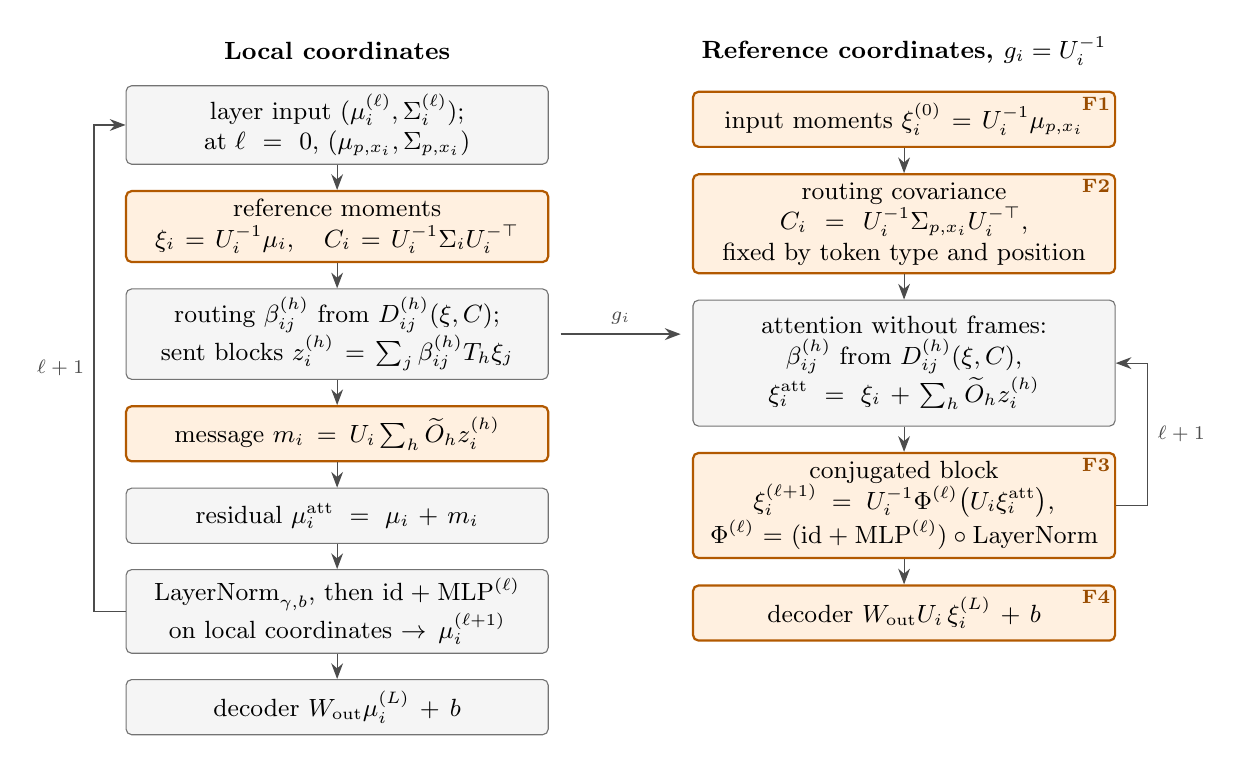
\begin{tikzpicture}[
  font=\small,
  box/.style={draw=black!55, rounded corners=2pt, fill=black!4, text width=5.15cm, align=center, inner sep=3pt, minimum height=7mm},
  frame/.style={box, draw=orange!70!black, fill=orange!12, thick},
  tag/.style={font=\scriptsize\bfseries, text=orange!60!black},
  arr/.style={-{Stealth[length=2mm]}, black!70},
  node distance=3.2mm]
% Left panel: local coordinates.
\node[font=\small\bfseries] (Lt) at (0,0) {Local coordinates};
\node[box, below=2mm of Lt] (L0) {layer input $(\mu_i^{(\ell)},\Sigma_i^{(\ell)})$; at $\ell=0$, $(\mu_{p,x_i},\Sigma_{p,x_i})$};
\node[frame, below=of L0] (L1) {reference moments\\ $\xi_i=U_i^{-1}\mu_i,\quad C_i=U_i^{-1}\Sigma_iU_i^{-\top}$};
\node[box, below=of L1] (L2) {routing $\beta_{ij}^{(h)}$ from $D_{ij}^{(h)}(\xi,C)$;\\ sent blocks $z_i^{(h)}=\sum_j\beta_{ij}^{(h)}T_h\xi_j$};
\node[frame, below=of L2] (L3) {message $m_i=U_i\sum_h\widetilde O_hz_i^{(h)}$};
\node[box, below=of L3] (L4) {residual $\mu_i^{\mathrm{att}}=\mu_i+m_i$};
\node[box, below=of L4] (L5) {$\operatorname{LayerNorm}_{\gamma,b}$, then $\mathrm{id}+\mathrm{MLP}^{(\ell)}$\\ on local coordinates $\to\mu_i^{(\ell+1)}$};
\node[box, below=of L5] (L6) {decoder $W_{\mathrm{out}}\mu_i^{(L)}+b$};
\foreach \a/\b in {L0/L1,L1/L2,L2/L3,L3/L4,L4/L5,L5/L6} \draw[arr] (\a) -- (\b);
\draw[arr] (L5.west) -- ++(-4mm,0) |- node[pos=0.25, left, font=\scriptsize] {$\ell+1$} (L0.west);
% Right panel: reference coordinates after g_i = U_i^{-1}.
\node[font=\small\bfseries] (Rt) at (7.2cm,0) {Reference coordinates, $g_i=U_i^{-1}$};
\node[frame, below=2mm of Rt] (R0) {input moments $\xi_i^{(0)}=U_i^{-1}\mu_{p,x_i}$};
\node[frame, below=of R0] (R1) {routing covariance $C_i=U_i^{-1}\Sigma_{p,x_i}U_i^{-\top}$,\\ fixed by token type and position};
\node[box, below=of R1, minimum height=16mm] (R2) {attention without frames:\\ $\beta_{ij}^{(h)}$ from $D_{ij}^{(h)}(\xi,C)$,\\ $\xi_i^{\mathrm{att}}=\xi_i+\sum_h\widetilde O_hz_i^{(h)}$};
\node[frame, below=of R2] (R3) {conjugated block $\xi_i^{(\ell+1)}=U_i^{-1}\Phi^{(\ell)}\bigl(U_i\xi_i^{\mathrm{att}}\bigr)$,\\ $\Phi^{(\ell)}=(\mathrm{id}+\mathrm{MLP}^{(\ell)})\circ\operatorname{LayerNorm}$};
\node[frame, below=of R3] (R4) {decoder $W_{\mathrm{out}}U_i\,\xi_i^{(L)}+b$};
\foreach \a/\b in {R0/R1,R1/R2,R2/R3,R3/R4} \draw[arr] (\a) -- (\b);
\draw[arr] (R3.east) -- ++(4mm,0) |- node[pos=0.25, right, font=\scriptsize] {$\ell+1$} (R2.east);
\node[tag, anchor=north east, inner sep=2pt] at (R0.north east) {F1};
\node[tag, anchor=north east, inner sep=2pt] at (R1.north east) {F2};
\node[tag, anchor=north east, inner sep=2pt] at (R3.north east) {F3};
\node[tag, anchor=north east, inner sep=2pt] at (R4.north east) {F4};
% Site transformation between the panels.
\draw[arr, thick] ([xshift=1.5mm]L2.east) -- node[above, font=\scriptsize] {$g_i$} ([xshift=-1.5mm]L2.east -| R2.west);
\end{tikzpicture}
\caption{Reference-coordinate form of the evaluated architecture. Shaded boxes are the places where the frames $U_i$ enter; $z_i^{(h)}=\sum_j\beta_{ij}^{(h)}T_h\xi_j$ is the routed sent block of head $h$ in reference coordinates and $\widetilde O_h$ the effective receiving map of the chart. Left: one evaluated block in local coordinates, where the frame enters at the reference moments and at the message $m_i$. Right: the same computation after the site transformation $g_i=U_i^{-1}$. Every routing cost and message factors through $(\xi_i,C_i)$, so attention acts without frames, as Eq.~\eqref{eq:relational_covariance} implies, and the frames remain only in the input moments (F1), the routing covariance (F2), the conjugated normalization and MLP (F3), and the decoder (F4). Each tag names the row of Table~\ref{tab:placeholder_interventions} that removes that role. Under moment matching, $C_i$ is fixed only at the input and is then updated frame-free from the routing weights.}
\label{fig:placeholder_reference_gauge}
\end{figure}

\section{Gaussian-KL Routing and Its Transformer Reductions}
\label{sec:transformer_comparison_summary}

The correspondence with standard attention starts from the learned comparison and content maps, rather than replacing them by the flat identification $\Omega_{ij}$. We establish an exact dual-coordinate form of the routing cost (Theorem~\ref{thm:dual_coordinates}), its reduction under stated covariance and bias conditions, and an exact identity for the resulting value/output aggregation. These are conditional equalities of attention operators; Table~\ref{tab:transformer_correspondence} summarizes them by status.

\subsection{The full Gaussian score and its query--key cross term}
\label{sec:dot_product_derivation}

Fix a layer, a head, and its nonempty allowed source sets; suppress the layer and head indices. Write $r=r_h$ and define the projected moments
\begin{equation}
a_i=S_Q\xi_i,\quad b_j=S_K\xi_j,\quad
V_{Q,i}=S_QC_iS_Q^\top,\quad V_{K,j}=S_KC_jS_K^\top.
\label{eq:projected_qk_moments}
\end{equation}
The state covariances are positive definite and both comparison maps have full row rank, so $V_{Q,i},V_{K,j}\succ0$. The Gaussian KL formula gives
\begin{align}
D_{ij}=\frac12\bigl[&\operatorname{Tr}(P_jV_{Q,i})
+a_i^\top P_ja_i-2a_i^\top P_jb_j+b_j^\top P_jb_j-r\nonumber\\
&+\log\det V_{K,j}-\log\det V_{Q,i}\bigr],
\qquad P_j=V_{K,j}^{-1}.
\label{eq:projected_full_kl}
\end{align}
Its mean compatibility has the dot-product factorization $a_i^\top(P_jb_j)$; the KL contains the negative of this term. In ambient local coordinates it is $\mu_i^\top B_{ij}\mu_j$ with the comparison tensor of Eq.~\eqref{eq:comparison_bilinear_tensor}. Thus independent learned $S_Q,S_K$ already supply distinct query and key observables. Neither is required to be a gauge-group element. The other terms retain covariance information: when $P_j$ varies with the source, $a_i^\top P_ja_i$ and $\operatorname{Tr}(P_jV_{Q,i})$ are generally pair dependent and cannot be discarded as row constants.

All of these terms are organized by one exact identity.
\begin{theorem}[Dual-coordinate form of Gaussian-KL routing]
\label{thm:dual_coordinates}
Write the query law in expectation coordinates and the key law in natural coordinates,
\begin{equation}
\eta_{Q,i}=\bigl(a_i,V_{Q,i}+a_ia_i^\top\bigr),\qquad
\theta_{K,j}=\bigl(P_jb_j,-\tfrac12P_j\bigr),\qquad
\langle\eta,\theta\rangle=\eta_1^\top\theta_1+\operatorname{Tr}(\eta_2\theta_2),
\end{equation}
and let $A(\theta_{K,j})=\tfrac12b_j^\top P_jb_j+\tfrac12\log\det V_{K,j}+\tfrac r2\log2\pi$ be the Gaussian log-partition, with conjugate $A^*(\eta_{Q,i})=-H(q_{Q,i})$. Then
\begin{equation}
D_{ij}=A(\theta_{K,j})+A^*(\eta_{Q,i})-\langle\eta_{Q,i},\theta_{K,j}\rangle,
\label{eq:dual_pairing}
\end{equation}
and the categorical optimizer is exactly $\beta_{ij}=\softmax_j\bigl(\langle\eta_{Q,i},\theta_{K,j}\rangle/\tau-A(\theta_{K,j})/\tau+\log\pi_{ij}\bigr)$: a dot product in $\mathbb R^{r+r(r+1)/2}$ between query expectation parameters and key natural parameters, with the key log-partition as a source bias. No covariance hypothesis is needed.
\end{theorem}
\begin{proof}
With $-H(q_{Q,i})=-\tfrac12\log\det(2\pi eV_{Q,i})$, expanding the right side of Eq.~\eqref{eq:dual_pairing} reproduces Eq.~\eqref{eq:projected_full_kl} term by term. This is the mixed form of the divergence between members of an exponential family \citep[Sec.~5.2, Eq.~(5.11)]{Wainwright2008}. The term $A^*(\eta_{Q,i})$ is constant on row $i$ and cancels in the softmax.
\end{proof}
Proposition~\ref{prop:projected_dot_product} is the case in which the second-order key coordinate $-\tfrac12P_j$ is shared, so that only the mean block $a_i^\top V_*^{-1}b_j$ of the pairing varies with the source.

\begin{proposition}[Projected Gaussian reduction to biased dot-product routing]
\label{prop:projected_dot_product}
Suppose all keys used by a head have the same projected covariance $V_{K,j}=V_*\succ0$. Let $\tau>0$, let each prior row be a probability distribution with $\pi_{ij}>0$ on its allowed support, and let costs be the uncapped Gaussian divergences. Define $\mathsf q_i=V_*^{-1/2}a_i$ and $\mathsf k_j=V_*^{-1/2}b_j$, using the symmetric positive-definite inverse square root. Then the exact categorical optimizer is
\begin{equation}
\beta_{ij}=\softmax_j\left(
\frac{\mathsf q_i^\top\mathsf k_j}{\tau}
-\frac{\|\mathsf k_j\|^2}{2\tau}
+\log\pi_{ij}\right).
\label{eq:main_dot_product_scope}
\end{equation}
The query covariances may differ across receivers. If, more strongly, $V_{Q,i}=V_{K,j}=\sigma_h^2I_r$, then $D_{ij}=\|a_i-b_j\|^2/(2\sigma_h^2)$.
\end{proposition}
\begin{proof}
Set $P_j=V_*^{-1}$ in Eq.~\eqref{eq:projected_full_kl}. The trace, query quadratic, dimension, and determinant terms are independent of $j$, except for $b_j^\top V_*^{-1}b_j$ and the cross term. Thus
\begin{equation}
D_{ij}=c_i+\tfrac12\|\mathsf k_j\|^2
-\mathsf q_i^\top\mathsf k_j,
\label{eq:projected_kl_row_decomposition}
\end{equation}
for a row constant $c_i$. Substitution into the categorical solution $\softmax_j(-D_{ij}/\tau+\log\pi_{ij})$ removes $c_i$. Under the stronger isotropic assumption the trace and log-determinant terms cancel and the remaining quadratic is the stated squared distance.
\end{proof}
Since $D_{ij}=\tfrac12\|\mathsf q_i-\mathsf k_j\|^2$ up to a row constant, routing with shared projected key covariance is L2 attention in whitened coordinates; under the stronger isotropic hypothesis it is the L2 self-attention of \citet{Kim2021Lipschitz}. Dot-product attention is recovered only when projected key norms are constant or compensated (Section~\ref{sec:bias_cancellation}).

\begin{remark}[Relation to Gaussian-mixture attention]
\label{rem:gaussian_mixture_attention}
Because the entropy $H(q_{Q,i})$ is constant on row $i$ and $D_{\mathrm{KL}}(q\|p)=-\mathbb E_q\log p-H(q)$,
\begin{equation}
\beta_{ij}=\softmax_j\bigl(\log\pi_{ij}+\mathbb E_{q_{Q,i}}[\log p_{K,j}]/\tau\bigr),
\end{equation}
the mean-field responsibility of a Gaussian mixture under an uncertain query. For a point query at $a_i$ it is the mixture responsibility of \citet{Movellan2020ProbabilisticTransformers} and \citet{Nguyen2022MGK}, and Eq.~\eqref{eq:projected_key_bias_compensation} below is the prior with which \citet[Eqs.~16 to 21]{Movellan2020ProbabilisticTransformers} recover dot-product attention. The query covariance adds $-\operatorname{Tr}(P_jV_{Q,i})/(2\tau)$, which depends on the pair whenever $P_j$ varies with the source.
\end{remark}

The hypotheses of Proposition~\ref{prop:projected_dot_product} concern the projected distributions, not merely isotropic ambient states. Even if $C_i=\sigma^2I_K$, a learned map has covariance $\sigma^2S_KS_K^\top$, which need not be isotropic. Shared $C_i=C$ across tokens does give a shared key covariance for fixed $S_K$ and therefore satisfies the weaker proposition. It places no equality requirement on $S_Q$ and $S_K$. Whitening then defines the effective learned maps $\widetilde S_Q=V_*^{-1/2}S_Q$ and $\widetilde S_K=V_*^{-1/2}S_K$. The simple choice $K=2r$, $S_Q=[I_r\ 0]$, $S_K=[0\ I_r]$, and $C_i=\sigma^2I_K$ demonstrates that distinct query and key observables can satisfy even the stronger isotropic assumptions. A trained state with source-dependent projected covariance need not satisfy either specialization.

\subsection{Exact bias cancellation, approximation, and temperature}
\label{sec:bias_cancellation}

Equation~\eqref{eq:main_dot_product_scope} becomes ordinary dot-product attention with the same source prior exactly when the squared key norms are constant on the allowed support. More generally, a desired base prior $\pi^0_{ij}$ can be reproduced algebraically by choosing
\begin{equation}
\pi_{ij}=
\frac{\pi^0_{ij}\exp(\|\mathsf k_j\|^2/(2\tau))}
{\sum_{k\in S_i}\pi^0_{ik}\exp(\|\mathsf k_k\|^2/(2\tau))}.
\label{eq:projected_key_bias_compensation}
\end{equation}
This is an explicit state-dependent compensation. It is not a positional prior fixed independently of the current key states, and it is not assumed to be implemented. A minimal counterexample shows why the condition matters: for $r=1$, $\tau=1$, $a_i=0$, keys $b_1=0,b_2=1$, shared unit variance, and uniform prior, ordinary dot-product routing gives $(1/2,1/2)$ while Gaussian routing gives $(1,e^{-1/2})/(1+e^{-1/2})$.

An approximation can be stated by bounding the remaining bias.
\begin{proposition}[Sharp routing perturbation bound]
\label{prop:sharp_bound}
For any row constant $c_i$, under the hypotheses of Proposition~\ref{prop:projected_dot_product}, define
\begin{equation}
\varepsilon_i=\max_{j\in S_i}
\frac{|\|\mathsf k_j\|^2-c_i|}{2\tau},\qquad
p_{ij}=\softmax_j\left(\mathsf q_i^\top\mathsf k_j/\tau+\log\pi_{ij}\right).
\label{eq:projected_bias_error}
\end{equation}
Then
\begin{equation}
\sum_j|\beta_{ij}-p_{ij}|\le2\tanh(\varepsilon_i/2)\le\min(\varepsilon_i,2),
\label{eq:projected_softmax_bound}
\end{equation}
with equality for two sources with $p_{i1}=1/(1+e^{\varepsilon_i})$ and key-norm offsets of $\pm\varepsilon_i$. The best row constant is the midrange, which gives $\varepsilon_i=(\max_j\|\mathsf k_j\|^2-\min_j\|\mathsf k_j\|^2)/(4\tau)$.
\end{proposition}
\begin{proof}
By Eq.~\eqref{eq:main_dot_product_scope}, $\beta_{ij}=p_{ij}e^{\delta_{ij}}/\sum_kp_{ik}e^{\delta_{ik}}$ with $\delta_{ij}=-(\|\mathsf k_j\|^2-c_i)/(2\tau)$, so $|\delta_{ij}|\le\varepsilon_i$. For $A\subseteq S_i$, the derivative of $\beta_i(A)$ in $\delta_{ik}$ is positive for $k\in A$ and negative otherwise, so $\beta_i(A)-p_i(A)$ is largest at $\delta_{ij}=\varepsilon_i$ on $A$ and $\delta_{ij}=-\varepsilon_i$ off $A$, where it equals $x(1-x)(e^{2\varepsilon_i}-1)/[1+x(e^{2\varepsilon_i}-1)]$ with $x=p_i(A)$. The maximum over $x$ is attained at $x=1/(1+e^{\varepsilon_i})$ and equals $\tanh(\varepsilon_i/2)$. Since $\sum_j|\beta_{ij}-p_{ij}|=2\max_A[\beta_i(A)-p_i(A)]$, the bound follows, and $2\tanh(\varepsilon_i/2)\le\min(\varepsilon_i,2)$ because $\tanh$ is bounded by one and by its argument. The midrange minimizes $\varepsilon_i$ over $c_i$.
\end{proof}
The ratio bound $e^{-2\varepsilon_i}\le\beta_{ij}/p_{ij}\le e^{2\varepsilon_i}$ remains available as a multiplicative statement.
Therefore uniform control $\varepsilon_i\to0$ suffices for rowwise convergence, including when the number of keys varies. For the conventional scale $\tau=\sqrt r$, this requires maximum squared-norm dispersion $o(\sqrt r)$ on the row support. High-dimensional relative concentration alone is insufficient: for independent standard Gaussian vectors, the squared norm has variance $2r$ and the dot product of independent vectors has variance $r$. Both residuals retain order-one fluctuations after division by $\sqrt r$. Coordinate LayerNorm followed by an arbitrary learned key map does not impose the required projected-key norm constancy.

Standard attention uses the comparison dimension \(r_h\) in its scale \(\sqrt{r_h}\) \citep[Sec.~3.2.1]{vaswani2017attention}. After whitening, the cross term has this conventional scale when \(\tau_h=\sqrt{r_h}\). For arbitrary positive \(\tau_h\), rescaling both effective query and key by \((\sqrt{r_h}/\tau_h)^{1/2}\) writes the same cross term with denominator \(\sqrt{r_h}\). Covariance scale has already entered through whitening and must not be counted a second time as temperature. Numerical modification of the KL cost lies outside the uncapped score identity unless it leaves every relevant cost unchanged.

Geometric dilation must also be separated from statistical sharpness. A passive rescaling of one frame block (Appendix~\ref{sec:heads_irreps}) transforms its mean, covariance, and frame together as $(\mu,\Sigma,U)\mapsto(c\mu,c^2\Sigma,cU)$, $c\ne0$. The reference moments and all routing costs are unchanged. At fixed projected means, changing a shared isotropic comparison covariance $\sigma_h^2I$ instead changes the statistical model and gives $D_{ij}^{(h)}=\|S_{Q,h}\xi_i-S_{K,h}\xi_j\|^2/(2\sigma_h^2)$. The logits then depend on $\sigma_h^2$ and $\tau_h$ only through $\sigma_h^2\tau_h$, so the two are not separately identifiable from routing. For general projected covariances, trace and determinant terms prevent reducing every covariance change to one scalar temperature.

\subsection{Value, output, and residual links}
\label{sec:value_aggregation}

For any routing weights, independently of the dot-product specialization, predictive content has the exact reference-coordinate form
\begin{align}
v_j^{(h)}&=T_h\xi_j,\qquad
z_i^{(h)}=\sum_j\beta_{ij}^{(h)}v_j^{(h)},\\
U_i^{-1}\mu_i^{\mathrm{att}}
&=r\xi_i+\sum_h\widetilde O_hz_i^{(h)}
=r\xi_i+\sum_{j,h}\beta_{ij}^{(h)}\widetilde O_hT_h\xi_j.
\label{eq:projected_transformer_residual}
\end{align}
Concatenate the $z_i^{(h)}$. Then $\sum_h\widetilde O_hz_i^{(h)}=\widetilde O\operatorname{concat}_h(z_i^{(h)})$, the usual multi-head output projection \citep[Sec.~3.2.2]{vaswani2017attention}. With column-vector conventions, the dictionary is $W_V^{(h)}=T_h$ and output blocks $W_O^{(h)}=\widetilde O_h$; the matrices in the original row-vector transformer convention are their transposes. In the affine chart $W_O=O$ is a free parameter. In the exponential chart with tiled heads, $W_O=e^{OT}W_V^{-1}$ is the same output projection reparametrized through a generator and restricted to the matrices for which $W_OW_V$ has a real logarithm (Section~\ref{sec:lie_orders}). In local coordinates the same operation is $\sum_{j,h}\beta_{ij}^{(h)}L_{ij}^{(h)}\mu_j$. Thus the content link is the framed value/output composition, not the query--key compatibility tensor.

Each head can read all $K$ coordinates and write into all $K$ output coordinates. The latent channel dimension limits the rank of an individual contribution, not its input or output support. Communication heads need not coincide with a partition into gauge-frame blocks; full-width maps can mix those blocks even when every $U_i$ is block diagonal. Equation~\eqref{eq:projected_transformer_residual}, together with Proposition~\ref{prop:projected_dot_product} and its bias conditions, supplies the conditional attention-layer correspondence. The explicit residual $r=1$ is part of the architecture of Section~\ref{sec:relational_run}; Theorem~\ref{thm:probabilistic_status} reads it as the persistence term of the predictive kernel of Eq.~\eqref{eq:predictive_kernel}, Section~\ref{sec:relational_run} reports that it is numerically inert in that trained model, and the chart comparison of Section~\ref{sec:chart_runs} uses $r=0$.

\subsection{Restricted rotary correspondence and the remaining stack}
\label{sec:rope}

Rotary position embedding (RoPE) applies position-dependent orthogonal rotations after query and key projection \citep{su2024roformer}. For an even comparison dimension, let $R_i$ be a block-diagonal matrix of planar rotations with angles proportional to position, so $R_i^\top R_j=R_{j-i}$. A declared comparison-space construction $a_i\mapsto R_i a_i$, $b_j\mapsto R_jb_j$ has cross term
\begin{equation}
(R_i a_i)^\top(R_jb_j)
=a_i^\top R_{j-i}b_j
=\xi_i^\top S_Q^\top R_{j-i}S_K\xi_j.
\label{eq:projected_rope_kernel}
\end{equation}
Rotating both projected laws gives, by Eq.~\eqref{eq:glk_invariance}, $D_{\mathrm{KL}}\bigl((R_i)_*q_{Q,i}\|(R_j)_*p_{K,j}\bigr)=D_{\mathrm{KL}}\bigl(q_{Q,i}\|(R_{j-i})_*p_{K,j}\bigr)$, a relative-position score for arbitrary projected covariances. The dot-product form with an unchanged key-norm bias requires only that the shared key covariance commute with every $R_\delta$; with distinct rotation frequencies this means $V_*=\bigoplus_k\lambda_kI_2$ over the rotation planes. Query covariance is unrestricted. If the rotations act on anisotropic projected laws rather than on means alone, the trace and query-quadratic terms of Eq.~\eqref{eq:projected_full_kl} also become functions of $i-j$ and contribute relative-position biases.

This identity does not automatically identify position rotations inside an ambient frame with ordinary post-projection RoPE. Moving an ambient positional map through $S_Q$ or $S_K$ requires the corresponding intertwining identities, such as $S_Qe^{-Y_i}=R_iS_Q$ and $S_Ke^{-Y_i}=R_iS_K$ for the positional factor of $U_i=e^{\phi_{x_i}}e^{Y_i}$; imposing the identity on the complete $U_i^{-1}$ would require every token factor to act trivially on the comparison row spaces. Arbitrary learned maps need not satisfy them. In addition, ordinary RoPE leaves value aggregation unrotated. The separated comparison and content maps allow this design to be specified, but one shared ambient positional frame acting through every $U_i^{-1}$ does not establish it. The relative rotation is a flat group-valued factor; the full projected compatibility remains a generally low-rank bilinear tensor, and the content link remains a separate operator.

Covariance may be retained as a routing state in a predictive architecture. Passing it unchanged through the mean residual does not compute the covariance of a Gaussian mixture or propagate uncertainty through normalization and the MLP. For example, a declared mixture of content laws with means $v_j$ and covariances $W_j$ would have covariance $\sum_j\beta_j[W_j+(v_j-\bar v)(v_j-\bar v)^\top]$, where $\bar v=\sum_j\beta_jv_j$. The predictive mean identity does not require this additional propagation rule; Eq.~\eqref{eq:predictive_kernel_covariance} gives its multi-head form for the predictive kernel.

\begin{table}[t]
\centering
\small
\renewcommand{\arraystretch}{1.1}
\begin{tabularx}{\textwidth}{@{}p{0.29\textwidth}X@{}}
\toprule
Correspondence & Exact scope or remaining condition \\
\midrule
\multicolumn{2}{@{}l}{\emph{Derived under stated conditions}}\\
Gaussian categorical routing & Exact optimizer for fixed costs, allowed support, and positive temperature; exact label posterior under a binary compatibility record \\
Query/key dot product & Exact dot product in dual coordinates, Eq.~\eqref{eq:dual_pairing}; reduces to the $r_h$-dimensional mean block under shared key covariance \\
Ordinary attention weights & Shared key covariance, matched scale, and constant or compensated key-norm bias; otherwise L2 attention in whitened coordinates \\
RoPE score & Relative dependence exact for arbitrary projected covariances when both laws rotate; dot-product form requires a shared key covariance that commutes with the rotations \\
\midrule
\multicolumn{2}{@{}l}{\emph{Identical by construction}}\\
Value/output aggregation & $T_h$ and $\widetilde O_h$ are the value and output maps; framed content-link identity at any fixed routing \\
Exponential content link & Output projection $e^{OT}T^{-1}$ of tiled heads: a reparametrization of $W_O$ on the real-logarithm domain, with orders separating flat transport, value path, and cross-head mixing \\
Multi-head organization & Full-width maps and output concatenation identity; no frame-block partition is required \\
\midrule
\multicolumn{2}{@{}l}{\emph{Not derived (architectural choices)}}\\
Predictive residual & Coefficient $r\in\{0,1\}$; $r=1$ is read as the persistence term of a predictive kernel and was numerically inert after training in the $K=256$ run; tiled exponential aggregation has no residual \\
Covariance, normalization, MLP, decoder & Separate processing choices; the linear decoder is a Gibbs readout of shared-covariance templates \\
\bottomrule
\end{tabularx}
\caption{Transformer correspondences for the projection-based architecture, grouped by status. The equalities concern the specified operators, not an identity between unrestricted model families.}
\label{tab:transformer_correspondence}
\end{table}

\section{Probabilistic Status of Routing and Content}
\label{sec:probabilistic_status}

The Gibbs row of Eq.~\eqref{eq:relational_routing} and the content update of Eq.~\eqref{eq:relational_predictive_residual} were stated as operations. This section derives the row from a declared local source model, shows that it is an exact posterior at every temperature, and shows that the content update with its residual is an exact predictive mean.

\subsection{Variational source selection}
\label{sec:mixture_derivation}
Fix a layer, head, and receiver, suppressing those indices. Let $q_{Q,i}(y)$ be the projected query law and $p_{K,j}(y)$ the candidate key laws. On a nonempty allowed support $S_i$, take positive probabilities $\pi_{ij}$ summing to one. The normalized local source model and factorized recognition law are
\begin{align}
\mathbb P_i(y,J=j)&=\pi_{ij}p_{K,j}(y),\label{eq:mixture_joint}\\
\mathbb Q_{i,\beta}(y,J=j)&=\beta_{ij}q_{Q,i}(y).\label{eq:mixture_posterior}
\end{align}
Here the Gaussian states are fixed values at the given context: they are computed from the prefix before routing and enter the local joint as data, so $p_{K,j}$ reads a state value rather than a recognition law being optimized, and $\beta_i$ is the only recognition variable. The receiver enters only through the query law, clamped as the recognition marginal of $y$. Hold the query law fixed during categorical minimization. Expanding the density ratio gives
\begin{align}
D_{\mathrm{KL}}(\mathbb Q_{i,\beta}\|\mathbb P_i)
&=\sum_{j\in S_i}\beta_{ij}D_{ij}
+\sum_{j\in S_i}\beta_{ij}\log\frac{\beta_{ij}}{\pi_{ij}},
\label{eq:mixture_free_energy}\\
D_{ij}&=D_{\mathrm{KL}}(q_{Q,i}\|p_{K,j}).
\label{eq:mixture_energy_entropy}
\end{align}
The categorical entropy belongs to this variational objective. The direction of $D_{ij}$ is fixed by the declared joint and the exclusive divergence: the key laws are the generative mixture components and the query law is the recognition factor. The inclusive divergence gives $D_{\mathrm{KL}}(\mathbb P_i\|\mathbb Q_{i,\beta})=D_{\mathrm{KL}}(\pi_i\|\beta_i)+\sum_j\pi_{ij}D_{\mathrm{KL}}(p_{K,j}\|q_{Q,i})$, whose minimizer is $\beta_i=\pi_i$ for all costs. The reverse cost $D_{\mathrm{KL}}(p_{K,j}\|q_{Q,i})$ follows from the joint $\pi_{ij}q_{Q,i}(y)$ with recognition $\beta_{ij}p_{K,j}(y)$; its reduction to a dot product requires a shared query covariance and retains a source-dependent bias. Symmetric divergences require both projected covariances to be shared.

At a declared temperature $\tau>0$, use
\begin{equation}
\mathcal A_i(\beta)=\sum_{j\in S_i}\beta_{ij}D_{ij}
+\tau D_{\mathrm{KL}}(\beta_i\|\pi_i).
\label{eq:F_align_canonical_tau}
\end{equation}
The Hessian $\tau\operatorname{diag}(1/\beta_{ij})$ is positive definite on nonzero simplex tangent directions. The Lagrange condition is
$D_{ij}+\tau(\log(\beta_{ij}/\pi_{ij})+1)+\lambda_i=0$.
For finite costs the unique minimizer is interior on $S_i$:
\begin{align}
\beta_{ij}^*&=\frac{\pi_{ij}\exp(-D_{ij}/\tau)}
{\sum_{k\in S_i}\pi_{ik}\exp(-D_{ik}/\tau)},
\label{eq:mixture_softmax_general}\\
\beta_{ij}^*&=\operatorname{softmax}_{j\in S_i}(-D_{ij}/\tau)
\quad\text{for uniform }\pi_i.
\label{eq:mixture_softmax}
\end{align}
Substitution gives $-\tau\log Z_i$, with
$Z_i=\sum_{j\in S_i}\pi_{ij}\exp(-D_{ij}/\tau)$, by the usual entropy-regularized variational calculation \citep{Boyd2004,Wainwright2008,Niculae2017Regularized}.
At $\tau=1$ this is the KL of the declared local joint; general temperature changes that objective. The categorical minimizer needs no gradient-based update of $q_i$. Local mixture normalization does not supply a population model or a language-model observation likelihood.

Complete-state alignment is a special comparison: for $S_Q=S_K=I_K$, common pushforward by $U_i$ gives
$D_{ij}=D_{\mathrm{KL}}(q_i\|(\Omega_{ij})_*q_j)$.
Independent lower-dimensional role measurements therefore extend the comparison beyond this frame-only case. For tied maps, $D_{ij}\le D_{\mathrm{KL}}(q_i\|(\Omega_{ij})_*q_j)$ by the data-processing inequality \citep[Thm.~9]{vanErvenHarremoes2014}, so a shared comparison coarse-grains complete-state alignment; for $S_Q\ne S_K$ no such bound holds, and identical states can have $D_{ij}>0$.

\subsection{Exact posterior and predictive mean}
\label{sec:exact_posterior}

\begin{theorem}[Exact probabilistic status of routing and content]
\label{thm:probabilistic_status}
Fix a layer and its input states, and let $D_{ij}^{(h)}\ge0$ be the routing costs.
\begin{enumerate}
\item For every $\tau_h>0$, give each receiver and head a source label $J_i^{(h)}$ with prior $\pi_i^{(h)}$ and a binary compatibility record $o_i^{(h)}$ with $P(o_i^{(h)}=1\mid J_i^{(h)}=j)=\exp(-D_{ij}^{(h)}/\tau_h)$. The joint is normalized on any source graph, and $P(J_i^{(h)}=j\mid o_i^{(h)}=1)=\beta_{ij}^{(h)}$ of Eq.~\eqref{eq:relational_routing}. The objective of Eq.~\eqref{eq:relational_routing_objective} is $\tau_h$ times the label free energy $D_{\mathrm{KL}}(\beta\|\pi_i^{(h)})-\sum_j\beta_j\log P(o_i^{(h)}=1\mid J_i^{(h)}=j)$, whose minimum is the surprisal $-\log P(o_i^{(h)}=1)$.
\item Let the head labels be independent with laws $\beta_i^{(h)}$, and take the directed kernel
\begin{equation}
k_i'\mid k,J_i\sim\mathcal N\Bigl(rk_i+\sum_hL_{iJ_i^{(h)}}^{(h)}k_{J_i^{(h)}},Q_i\Bigr),\qquad r\in\{0,1\},\quad Q_i\succeq0,
\label{eq:predictive_kernel}
\end{equation}
which is normalized for any link rank, as a degenerate Gaussian when $Q_i$ is singular. At state values $k_j=\mu_j$ its predictive mean is $\mu_i^{\mathrm{att}}$ of Eq.~\eqref{eq:relational_predictive_residual}. With independent source states $k_j\sim\mathcal N(\mu_j,\Sigma_j)$, the self edge included, its moment-matched covariance in reference coordinates is
\begin{equation}
\begin{aligned}
C_i^{\mathrm{att}}={}&\widetilde Q_i+r\Bigl[C_i+\sum_h\beta_{ii}^{(h)}\bigl(M_hC_i+C_iM_h^\top\bigr)\Bigr]
+\sum_j\sum_{h,h'}c_{ij}^{hh'}M_hC_jM_{h'}^\top\\
&+\sum_h\Bigl[\sum_j\beta_{ij}^{(h)}n_{ij}^{(h)}n_{ij}^{(h)\top}-\bar n_i^{(h)}\bar n_i^{(h)\top}\Bigr],
\end{aligned}
\label{eq:predictive_kernel_covariance}
\end{equation}
where $\widetilde Q_i=U_i^{-1}Q_iU_i^{-\top}$, $M_h=\widetilde O_hT_h$, $c_{ij}^{hh}=\beta_{ij}^{(h)}$, $c_{ij}^{hh'}=\beta_{ij}^{(h)}\beta_{ij}^{(h')}$ for $h\ne h'$, $n_{ij}^{(h)}=M_h\xi_j$, and $\bar n_i^{(h)}=\sum_j\beta_{ij}^{(h)}n_{ij}^{(h)}$. The local covariance $U_iC_i^{\mathrm{att}}U_i^\top$ obeys the passive law.
\end{enumerate}
\end{theorem}
\begin{proof}
(1) Because $D_{ij}^{(h)}\ge0$, each record kernel takes values in $(0,1]$ and is normalized. Records attached to different receivers and heads are conditionally independent children of the states and labels, so the joint is normalized. Bayes' rule gives $P(J=j\mid o=1)=\pi_{ij}e^{-D_{ij}/\tau}/\sum_k\pi_{ik}e^{-D_{ik}/\tau}$, which is Eq.~\eqref{eq:relational_routing}. Since $-\log P(o=1\mid J=j)=D_{ij}/\tau$, the label free energy equals $\tau^{-1}$ times the objective, and its minimum is $-\log\sum_j\pi_{ij}e^{-D_{ij}/\tau}=-\log P(o=1)$.
(2) Write $X=rk_i+\sum_hL_{iJ^{(h)}}^{(h)}k_{J^{(h)}}$. Conditioning on the labels gives $\mathbb E[X\mid J]=r\mu_i+\sum_hL^{(h)}_{iJ^{(h)}}\mu_{J^{(h)}}$, whose average over the independent labels is $\mu_i^{\mathrm{att}}$. By the law of total covariance, $\operatorname{Cov}X=\mathbb E\operatorname{Cov}(X\mid J)+\operatorname{Cov}\mathbb E(X\mid J)$. Given the labels, each distinct source $s$ contributes $A_s\Sigma_sA_s^\top$, with $A_i=rI+\sum_h\mathbf 1[J^{(h)}=i]L_{ii}^{(h)}$ and $A_s=\sum_h\mathbf 1[J^{(h)}=s]L_{is}^{(h)}$ for $s\ne i$. Averaging the indicator products with $\mathbb E\bigl(\mathbf 1[J^{(h)}=s]\mathbf 1[J^{(h')}=s]\bigr)=c_{is}^{hh'}$ gives the terms in $C_i$, $\beta_{ii}^{(h)}$, and $c_{ij}^{hh'}$, and independence of the labels across heads gives the spread term. Conjugating by $U_i^{-1}$ removes every frame, since $L_{ij}^{(h)}\Sigma_jL_{ij}^{(h')\top}=U_iM_hC_jM_{h'}^\top U_i^\top$, and adding $Q_i$ completes the kernel covariance.
\end{proof}
The record is a declared modeling event of the kind used for optimality variables in control as inference \citep{ToussaintStorkey2006,Kappen2012,Levine2018}; it is not an observed datum. Exactness of this kind is available for any nonnegative cost, so item (1) shows that Gibbs routing is consistent with exact inference, not that attention must be inference. Covariance passthrough with $r=1$ retains only the term $C_i$ of Eq.~\eqref{eq:predictive_kernel_covariance}. The derivation of item (2) leaves $T_h$, $\widetilde O_h$, and $Q_i$ free; it holds in every chart of Eq.~\eqref{eq:lie_three_charts}; it declares the persistence coefficient, additivity across heads, and one label for both the compatibility record and the content channel; and it does not cover the normalization and MLP maps or the collapse of the predictive mixture to a point state between layers.

The implemented moment-matched contract evaluates Eq.~\eqref{eq:predictive_kernel_covariance} with the reference floor $\widetilde Q_i=\epsilon_Q\operatorname{Tr}(C_i)I/K$, so that $Q_i=\epsilon_Q\operatorname{Tr}(C_i)U_iU_i^\top/K$ transforms as a covariance because $\operatorname{Tr}C_i$ is invariant under the passive action. The output then satisfies $\lambda_{\min}(C_i^{\mathrm{att}})\ge\epsilon_Q\operatorname{Tr}(C_i)/K$ whatever the routing and the rank of $M_h$. With $r=0$ the covariance is that of the message alone plus the floor; with $r=1$ the self-edge cross terms $\beta_{ii}^{(h)}(M_hC_i+C_iM_h^\top)$ can be indefinite, so no monotonicity in depth holds in general. When only the local diagonal of the covariance is stored, matching marginal variances is the projection that minimizes $D_{\mathrm{KL}}(p\|q)$ over diagonal Gaussian $q$, and it does not commute with arbitrary $\mathrm{GL}(K)$ congruences, so the passive law applies before that projection.

For fixed $q_{Q,i}$ the optimizer of Eq.~\eqref{eq:mixture_softmax_general} minimizes $\mathbb E_{y\sim q_{Q,i}}D_{\mathrm{KL}}\bigl(\beta_i\|p_i^{(\tau)}(\cdot\mid y)\bigr)$ with $p_i^{(\tau)}(j\mid y)\propto\pi_{ij}p_{K,j}(y)^{1/\tau}$: it is the normalized geometric mean of the pointwise source posteriors under the query law. The posterior-predictive source probability $\mathbb E_{y\sim q_{Q,i}}\mathbb P_i(J=j\mid y)$ minimizes the reverse expected divergence. It is also the unrestricted minimizer of the KL to $\mathbb P_i$ over joints whose $y$-marginal is clamped to $q_{Q,i}$, and it generally differs from the Gibbs row, as for the readout of Appendix~\ref{sec:prior_bank_readout}. Apart from a row constant, the query covariance enters $D_{ij}$ only through the trace term of Eq.~\eqref{eq:projected_full_kl}. That term penalizes sources whose key laws are precise along the uncertain directions of the query, and it drops out when key covariances are shared. A broad query law therefore does not flatten Gibbs routing.

\begin{remark}[Noisy-query routing]
\label{rem:noisy_query}
A rule under which query uncertainty does flatten routing requires a different local model, in which the projected query mean is data. Under source $j$, let $y\sim p_{K,j}$ and let the observed query mean be $a_i=y+\varepsilon$ with independent noise $\varepsilon\sim\mathcal N(0,V_{Q,i})$. Then $p(a_i\mid J=j)=\mathbb E_{y\sim q_{Q,i}}[p_{K,j}(y)]=\mathcal N(a_i;b_j,V_{Q,i}+V_{K,j})$, the expected likelihood kernel of the two laws \citep[Secs.~2.1 and~3.1]{Jebara2004ProbabilityProduct}, and Bayes' rule gives the exact posterior
\begin{equation}
P(J=j\mid a_i)=\frac{\pi_{ij}\mathcal N(a_i;b_j,V_{Q,i}+V_{K,j})}{\sum_{k\in S_i}\pi_{ik}\mathcal N(a_i;b_k,V_{Q,i}+V_{K,k})}.
\label{eq:noisy_query_routing}
\end{equation}
At unit temperature, Gibbs routing normalizes $\pi_{ij}\exp\mathbb E_{q_{Q,i}}[\log p_{K,j}]$, whereas Eq.~\eqref{eq:noisy_query_routing} normalizes $\pi_{ij}\mathbb E_{q_{Q,i}}[p_{K,j}]$; in the point-query limit both give the mixture responsibility of Remark~\ref{rem:gaussian_mixture_attention}. With shared key covariance $V_*$, Eq.~\eqref{eq:noisy_query_routing} is Eq.~\eqref{eq:main_dot_product_scope} at $\tau=1$ with $V_*$ replaced by $V_{Q,i}+V_*$, so the query covariance enters as a receiver-dependent whitening that tempers the row. For $r=1$, keys $b_1=0$ and $b_2=1$ with unit variance, $a_i=0$, and a uniform prior, the unit-temperature Gibbs weight on the first source is $(1+e^{-1/2})^{-1}\approx0.622$ for every query variance $v$, whereas Eq.~\eqref{eq:noisy_query_routing} gives $(1+e^{-1/(2+2v)})^{-1}$, which is $0.562$ at $v=1$ and $0.511$ at $v=10$. The weights depend on the states only through projected moments, and a common invertible map of the comparison space multiplies every term by the same Jacobian factor, so they share the invariances of Theorem~\ref{thm:reference_moments}. A temperature can be introduced through the binary record of Theorem~\ref{thm:probabilistic_status} after a row shift that makes the cost $-\log\mathcal N(a_i;b_j,V_{Q,i}+V_{K,j})$ nonnegative. The rule is a different routing operator rather than a reading of Eq.~\eqref{eq:relational_routing}, and the evaluated model does not implement it.
\end{remark}

\subsection{Content laws and the shared-latent alternative}
\label{sec:content_laws}

For one head, $z_i^{(h)}$ is exactly the mean of a declared mixture of content laws with means $T_h\xi_j$ and weights $\beta_{ij}$. A normalized local construction makes the limited probabilistic interpretation explicit. At fixed context, let $p_{K,j}(y)$ be the comparison densities of Eq.~\eqref{eq:relational_key_law}, and choose normalized content laws $\nu_j(\zeta)$ with those content means. Then
\begin{align}
\mathbb P_i(j,y,\zeta)&=\pi_{ij}p_{K,j}(y)\nu_j(\zeta),\\
\mathbb Q_{i,\beta}(j,y,\zeta)&=\beta_jq_{Q,i}(y)\nu_j(\zeta),\\
D_{\mathrm{KL}}(\mathbb Q_{i,\beta}\|\mathbb P_i)
&=\sum_j\beta_jD_{\mathrm{KL}}(q_{Q,i}\|p_{K,j})
+D_{\mathrm{KL}}(\beta\|\pi_i).
\label{eq:relational_normalized_model}
\end{align}
The identity follows by cancellation of $\nu_j$ in the density ratio and integration of normalized factors. It recovers the uncapped routing objective at $\tau_h=1$. Since every normalized $\nu_j$ cancels, this construction permits a chosen content bank but does not select its means, $T_h$, $\widetilde O_h$, or the residual. At general $\tau_h$, Eq.~\eqref{eq:relational_routing_objective} is the declared entropy-regularized extension, not the KL of this same joint without additional modeling changes; the binary compatibility record of Theorem~\ref{thm:probabilistic_status} realizes it exactly at every temperature. The identity determines routing within the declared joint; a predictive architecture requires additional choices.

The independent-content construction also distinguishes two measurements of a distribution from two observations of one latent draw. If $X_j\sim\mathcal N(\xi_j,C_j)$, $Y=S_KX_j+\varepsilon$ with independent Gaussian noise $\varepsilon\sim\mathcal N(0,R)$, $R\succeq0$, and $V=T X_j$, then Gaussian conditioning instead gives \citep{petersen2012matrix}
\begin{equation}
\mathbb E[V\mid Y=y,J=j]
=T\xi_j+TC_jS_K^\top(S_KC_jS_K^\top+R)^{-1}(y-S_K\xi_j).
\label{eq:relational_shared_latent_correction}
\end{equation}
Thus uncorrected values $T\xi_j$ do not generally equal shared-latent conditional means. Overlapping transmitting and comparison subspaces are permitted, but they do not remove this correlation term. The mixture-mean readout in Eq.~\eqref{eq:relational_predictive_residual} specifies a different statistical operation from this shared-latent conditioning law. With $R=0$ and the query law as the recognition of $Y$, this model gives the same routing objective and the pair-dependent content $T\bigl(\xi_j+R_{K,j}(S_Q\xi_i-S_K\xi_j)\bigr)$, where $R_{K,j}=C_jS_K^\top(S_KC_jS_K^\top)^{-1}$ is the key-side analogue of the lift in Eq.~\eqref{eq:comparison_gaussian_lift}. The uncorrected value is recovered for every query exactly when $TC_jS_K^\top=0$.

The same variational reading covers the decoder. The linear decoder of Eq.~\eqref{eq:predictive_linear_decoder} is exactly the unit-temperature Gibbs readout of shared-covariance Gaussian templates; Appendix~\ref{sec:prior_bank_readout} derives this identity and develops the Gaussian-bank readout with class-specific covariances.

\section{Receiver Inference over the Same Channels}
\label{sec:receiver_inference}

Section~\ref{sec:probabilistic_status} reads content predictively: each head's routed message is averaged, and the predictive mean replaces or increments the receiver's state. The same channels can instead be read as evidence about the receiver. The receiver holds a Gaussian prior, each head observes the receiver through a receiving measurement, and the routed source messages are the observations, so the update is a variational posterior. This section derives that receiver energy and its exact minimizer, states when the predictive head sum is its limit, and records the realization used in Section~\ref{sec:chart_runs}. Routing is computed from the comparison laws as before and held fixed during the update.

\subsection{The receiver episode and the channel likelihood}
\label{sec:rec_channel}

A receiver episode snapshots the incoming states $(\bar\xi_j,\bar C_j)$, the routing weights, and the frames of one layer. It then moves each receiver's state $(\xi,C)$ against an energy $F_i(\xi,C)$ with the snapshot held fixed in value, while the outer supervised graph through the snapshot remains attached. The frames do not change within the episode, so $(\mu,\Sigma)\mapsto(\xi,C)$ is a fixed linear reparametrization. Every energy below is a function of reference moments. Its local gradients are $\nabla_\mu F=U_i^{-\top}\nabla_\xi F$ and $\nabla_\Sigma F=U_i^{-\top}(\nabla_CF)U_i^{-1}$, and the Gaussian Fisher natural gradient $(\Sigma\nabla_\mu F,2\Sigma\nabla_\Sigma F\Sigma)$ equals the reference natural gradient $(C\nabla_\xi F,2C\nabla_CFC)$ mapped by $U_i$, with $U_i^\top$ on the right of the covariance term. A Fisher step taken in local coordinates is therefore the same step taken in reference coordinates and mapped back, because the Fisher metric of the Gaussian family is invariant under affine reparametrization of the sample space \citep{Amari1998}. We work in reference coordinates and suppress the receiver index.

Head $h$ observes the receiver through a receiving measurement $\mathsf P_h\in\mathbb R^{s_h\times K}$, and the message of source $j$, with the source state marginalized, predicts that measurement through a channel with noise $Q_h^{\mathrm{ch}}\succeq0$:
\begin{equation}
\begin{gathered}
\mathsf P_hx=T_hx_j+\epsilon,\qquad x_j\sim\mathcal N(\bar\xi_j,\bar C_j),\qquad \epsilon\sim\mathcal N(0,Q_h^{\mathrm{ch}}),\\
p(T_h\bar\xi_j\mid x)=\mathcal N\bigl(T_h\bar\xi_j;\mathsf P_hx,R_{hj}\bigr),\qquad R_{hj}=T_h\bar C_jT_h^\top+Q_h^{\mathrm{ch}}.
\end{gathered}
\label{eq:rec_channel_model}
\end{equation}
With the routing weights declared as likelihood powers $w_{hj}=\lambda_\beta\beta_{ij}^{(h)}$, $\lambda_\beta>0$, and a Gaussian prior $p=\mathcal N(\xi_p,C_p)$ with coefficient $\lambda_\alpha>0$, the receiver energy is
\begin{equation}
F(\xi,C)=\lambda_\alpha D_{\mathrm{KL}}\bigl(\mathcal N(\xi,C)\|\mathcal N(\xi_p,C_p)\bigr)+\sum_{h,j}w_{hj}\mathbb E_{x\sim\mathcal N(\xi,C)}\bigl[-\log\mathcal N(T_h\bar\xi_j;\mathsf P_hx,R_{hj})\bigr].
\label{eq:rec_channel_energy}
\end{equation}

\begin{proposition}[Closed-form channel receiver]
\label{prop:rec_closed_form}
Let $C_p\succ0$ and $R_{hj}\succ0$, and put
\begin{equation}
\begin{gathered}
W_h=\sum_jw_{hj}R_{hj}^{-1},\qquad \omega_h=\sum_jw_{hj}R_{hj}^{-1}T_h\bar\xi_j,\\
\Lambda=\lambda_\alpha C_p^{-1}+\sum_h\mathsf P_h^\top W_h\mathsf P_h,\qquad
\eta=\lambda_\alpha C_p^{-1}\xi_p+\sum_h\mathsf P_h^\top\omega_h.
\end{gathered}
\label{eq:rec_stats}
\end{equation}
Then
\begin{equation}
F(\xi,C)=\tfrac12\operatorname{Tr}(\Lambda C)+\tfrac12\xi^\top\Lambda\xi-\eta^\top\xi-\tfrac{\lambda_\alpha}{2}\log\det C+\mathrm{const},
\label{eq:rec_quadratic}
\end{equation}
$F$ is strictly convex on $\mathbb R^K\times\{C\succ0\}$, and its unique minimizer is
\begin{equation}
\xi^\star=\Lambda^{-1}\eta,\qquad C^\star=\lambda_\alpha\Lambda^{-1}.
\label{eq:rec_minimizer}
\end{equation}
Equivalently, $F=\lambda_\alpha D_{\mathrm{KL}}(\mathcal N(\xi,C)\|p_{\mathrm{pow}})+\mathrm{const}$, where $p_{\mathrm{pow}}(x)\propto p(x)\prod_{h,j}p(T_h\bar\xi_j\mid x)^{w_{hj}/\lambda_\alpha}$ is the normalized Gaussian power posterior with mean $\xi^\star$ and covariance $C^\star$.
\end{proposition}
\begin{proof}
For a Gaussian likelihood, $\mathbb E_{\mathcal N(\xi,C)}[-\log\mathcal N(y;\mathsf Px,R)]=\tfrac12(y-\mathsf P\xi)^\top R^{-1}(y-\mathsf P\xi)+\tfrac12\operatorname{Tr}(\mathsf P^\top R^{-1}\mathsf PC)+\tfrac12\log\det(2\pi R)$, and the Gaussian divergence is $\tfrac12[\operatorname{Tr}(C_p^{-1}C)+(\xi-\xi_p)^\top C_p^{-1}(\xi-\xi_p)-K+\log\det C_p-\log\det C]$. Collecting terms gives Eq.~\eqref{eq:rec_quadratic}. The expected log-likelihoods contain no entropy of the receiver, which enters once, through the prior divergence. The energy is a strictly convex quadratic in $\xi$ plus a function of $C$ that is linear apart from the strictly convex term $-\tfrac{\lambda_\alpha}2\log\det C$, and its gradients $\Lambda\xi-\eta$ and $\tfrac12(\Lambda-\lambda_\alpha C^{-1})$ vanish exactly at Eq.~\eqref{eq:rec_minimizer}. Finally, $F/\lambda_\alpha=\mathbb E_q[\log q-\log p-\sum_{h,j}(w_{hj}/\lambda_\alpha)\log p(T_h\bar\xi_j\mid x)]$ up to a constant, which is $D_{\mathrm{KL}}(q\|p_{\mathrm{pow}})$ minus the logarithm of the normalizer of $p_{\mathrm{pow}}$, and the product of the Gaussian prior with Gaussian likelihood powers is Gaussian with precision $\Lambda/\lambda_\alpha$ and information vector $\eta/\lambda_\alpha$.
\end{proof}

\begin{corollary}[Properties of the channel receiver]
\label{cor:rec_properties}
\begin{enumerate}
\item The receiver entropy enters with the single coefficient $\lambda_\alpha$, so $C^\star$ is the covariance of the declared power posterior. At $\lambda_\alpha=1$ and unit weights the update is the conjugate linear-Gaussian update \citep[Sec.~2.3.3]{Bishop2006}, and the Gaussian variational optimum is exact because the target is Gaussian \citep{OpperArchambeau2009}.
\item With $Q_h^{\mathrm{ch}}=0$ the energy is finite whenever $T_h$ has full row rank, because then $T_h\bar C_jT_h^\top\succ0$. A positive channel floor guards against loss of rank as $T_h$ is learned; it is not needed for finiteness.
\item The likelihoods depend on $x$ only through $\mathsf P_hx$. On $V_0=\bigcap_h\ker\mathsf P_h$, the directions that no head observes, the posterior conditional law given the observed component equals the prior conditional law, and if $C_p$ does not couple $V_0$ to its orthogonal complement, the posterior marginal on $V_0$ equals the prior marginal. No head imposes a value on $V_0$.
\item At $C=C^\star$, $C\Lambda=\lambda_\alpha I$, so the explicit Fisher mean step $\xi\leftarrow\xi-\varepsilon C(\Lambda\xi-\eta)$ contracts exactly for $0<\varepsilon<2/\lambda_\alpha$, and $\varepsilon=1/\lambda_\alpha$ is the Newton step.
\end{enumerate}
\end{corollary}
\begin{proof}
Item 1 restates Proposition~\ref{prop:rec_closed_form}. For item 2, $y^\top T_h\bar C_jT_h^\top y=(T_h^\top y)^\top\bar C_j(T_h^\top y)>0$ for $y\ne0$. For item 3, decompose $x=u+v$ with $u\in V_0^\perp$ and $v\in V_0$. Every likelihood depends on $x$ only through $\mathsf P_hu$, so $p_{\mathrm{pow}}(v\mid u)=p(v\mid u)$; if the prior factorizes over $V_0^\perp\oplus V_0$, so does $p_{\mathrm{pow}}$, and its marginal on $V_0$ is the prior marginal. For item 4, the step maps the error $e=\xi-\xi^\star$ to $(I-\varepsilon C\Lambda)e=(1-\varepsilon\lambda_\alpha)e$ at $C=C^\star$.
\end{proof}

\subsection{The receiving measurement and the predictive limit}
\label{sec:rec_predictive_limit}

The posterior moves the state along the gain $\Lambda^{-1}\mathsf P_h^\top W_h=(C^\star/\lambda_\alpha)\mathsf P_h^\top W_h$, as in a Kalman update, so the receiving interface of this energy is the measurement $\mathsf P_h$ rather than a free write-back map. The implementation ties $\mathsf P_h=\widetilde O_h^\top$, the transposed effective receiving map of the chart in use. This keeps the stored parameters and their block-identity initialization and gives the following limit.

\begin{proposition}[Predictive limit]
\label{prop:rec_predictive_limit}
Assume $\mathsf P_h=\widetilde O_h^\top$ with $\widetilde O_h^\top\widetilde O_g=\delta_{hg}I_{s_h}$ and $\sum_hs_h=K$, so that $\sum_h\widetilde O_h\widetilde O_h^\top=I_K$, assume $R_{hj}=R_h$ for every source, and let $\lambda_\alpha C_p^{-1}\to0$ and $\lambda_\alpha C_p^{-1}\xi_p\to0$. Then
\begin{equation}
\xi^\star\to\sum_h\widetilde O_h\sum_j\beta_{ij}^{(h)}T_h\bar\xi_j,
\label{eq:rec_predictive_limit}
\end{equation}
the residual-free predictive head sum of Eq.~\eqref{eq:relational_predictive_residual} in reference coordinates.
\end{proposition}
\begin{proof}
In the limit, $\Lambda=\sum_h\widetilde O_h(\lambda_\beta R_h^{-1})\widetilde O_h^\top$ and $\eta=\sum_h\widetilde O_h\lambda_\beta R_h^{-1}\sum_j\beta_{ij}^{(h)}T_h\bar\xi_j$, using $\sum_j\beta_{ij}^{(h)}=1$. Both are block diagonal in the orthonormal basis formed by the columns of the $\widetilde O_h$, and solving blockwise gives $\widetilde O_h^\top\xi^\star=\sum_j\beta_{ij}^{(h)}T_h\bar\xi_j$.
\end{proof}

Each relaxed hypothesis has a definite meaning. With source-dependent channel covariances, the channel mean of head $h$ becomes the precision-weighted average $(\sum_j\beta_{ij}^{(h)}R_{hj}^{-1})^{-1}\sum_j\beta_{ij}^{(h)}R_{hj}^{-1}T_h\bar\xi_j$, so confident senders count for more than their routing weight. Overlapping heads fuse their measurements by least squares. A finite prior blends the prior mean and the messages with a gain set by their precisions. For an isotropic prior precision $\lambda_\alpha C_p^{-1}=aI$ and message evidence of precision $\ell$ on the range $W$ of the measurements, $\sum_h\mathsf P_h^\top W_h\mathsf P_h=\ell P_W$ and $\sum_h\mathsf P_h^\top\omega_h=\ell P_Wm$ with $P_W$ the orthogonal projector onto $W$, the minimizer is
\begin{equation}
\xi^\star=(I-P_W)\xi_p+P_W\frac{a\xi_p+\ell m}{a+\ell}.
\label{eq:rec_fusion_residual}
\end{equation}
The coefficient of the prior state is its share of precision, $a/(a+\ell)$, on observed directions and one on unobserved directions, and the complement-preserving aggregation of Proposition~\ref{prop:lie_complement_persistence} is the limit $\ell/a\to\infty$ when its splitting is orthogonal. The posterior covariance $C^\star=\lambda_\alpha\Lambda^{-1}$ depends on the context but omits the between-source spread of the moment-matched predictive covariance, because geometric pooling of likelihoods differs from marginalizing a categorical predictive mixture. In the exponential chart the tied measurement has the zeroth-order part $(T^{-1})_{:,h}^\top$, which reads through $T^{-\top}$ and agrees with the head-routed flat transport of Proposition~\ref{prop:lie_order_zero} only when $T$ is orthogonal; tying the chart into the measurement is an implementation choice, not a consequence of the exponential construction.

\subsection{Updates, outer derivatives, and the profiled coupling}
\label{sec:rec_updates}

\begin{proposition}[Natural-parameter flow]
\label{prop:rec_flow}
For an energy of the form of Eq.~\eqref{eq:rec_quadratic} with an entropy coefficient $c_{\mathrm H}>0$ in place of $\lambda_\alpha$, the Fisher flow $\dot\xi=-C(\Lambda\xi-\eta)$, $\dot C=c_{\mathrm H}C-C\Lambda C$ has the exact solution
\begin{equation}
J(t)=(1-\rho)J(0)+\rho\Lambda/c_{\mathrm H},\qquad
\vartheta(t)=(1-\rho)\vartheta(0)+\rho\eta/c_{\mathrm H},\qquad
\rho=1-e^{-c_{\mathrm H}t},
\label{eq:rec_flow}
\end{equation}
in the natural parameters $J=C^{-1}$ and $\vartheta=C^{-1}\xi$. Every iterate with $\rho\in[0,1]$ is positive definite, the energy does not increase along the flow, and $\rho=1$ gives the minimizer $(\Lambda^{-1}\eta,c_{\mathrm H}\Lambda^{-1})$.
\end{proposition}
\begin{proof}
$\dot J=-J\dot CJ=\Lambda-c_{\mathrm H}J$ and $\dot\vartheta=\dot J\xi+J\dot\xi=\eta-c_{\mathrm H}\vartheta$ are linear with constant coefficients. A convex combination of positive-definite matrices is positive definite. Along the flow, $\tfrac{d}{dt}F=-\nabla_\xi F^\top C\nabla_\xi F-2\operatorname{Tr}(C\nabla_CFC\nabla_CF)\le0$, since $c_{\mathrm H}C-C\Lambda C=-2C\nabla_CFC$.
\end{proof}

With the snapshot fixed in value, the closed form, $\rho=1$, completes a receiver episode in one solve, and further iterations leave it unchanged when the coupling is constant. Its outer derivatives follow by implicit differentiation, $d\xi^\star=\Lambda^{-1}\bigl(d\eta-(d\Lambda)\xi^\star\bigr)$ and $dC^\star=(d\lambda_\alpha)\Lambda^{-1}-\lambda_\alpha\Lambda^{-1}(d\Lambda)\Lambda^{-1}$, which automatic differentiation through a Cholesky solve computes. This removes the step-size restriction of the explicit step, but it does not bound every outer derivative of the network. Partial damping $\rho<1$ descends the frozen energy in the full family: with a scalar coefficient the energy equals $c_{\mathrm H}D_{\mathrm{KL}}(q\|q^\star)$ up to a constant, with $q^\star=\mathcal N(\Lambda^{-1}\eta,c_{\mathrm H}\Lambda^{-1})$, and along the segment $\theta_\rho=(1-\rho)\theta_0+\rho\theta^\star$ of natural parameters with log-partition $A$, $\tfrac{d}{d\rho}D_{\mathrm{KL}}(q_{\theta_\rho}\|q^\star)=-(1-\rho)\delta^\top\nabla^2A(\theta_\rho)\delta\le0$ with $\delta=\theta^\star-\theta_0$.

When only local variances $s_k$ are stored, the energy restricted to the diagonal family separates in the variances as $\tfrac12\sum_k(\Lambda_{\mathrm{loc}})_{kk}s_k-\tfrac{c_{\mathrm H}}2\sum_k\log s_k$, with $\Lambda_{\mathrm{loc}}=U_i^{-\top}\Lambda U_i^{-1}$ and $\eta_{\mathrm{loc}}=U_i^{-\top}\eta$, so its exact restricted minimizer is $\mu^\star=\Lambda_{\mathrm{loc}}^{-1}\eta_{\mathrm{loc}}$ and $s_k^\star=c_{\mathrm H}/(\Lambda_{\mathrm{loc}})_{kk}$. Interpolating natural parameters does not stay in the diagonal family when $\Lambda_{\mathrm{loc}}$ is dense, and the coordinatewise damping $s_k^{-1}\mapsto(1-\rho)s_k^{-1}+\rho(\Lambda_{\mathrm{loc}})_{kk}/c_{\mathrm H}$ carries no descent guarantee. For $\Lambda=\bigl(\begin{smallmatrix}1&0.99\\0.99&1\end{smallmatrix}\bigr)$, $\eta=0$, $c_{\mathrm H}=1$, mean $(5,-5)$, variances $(1/2,2)$, and $\rho=1/2$, the frozen energy without constants rises from $1.500$ to $2.503$, while $\rho=1$ lowers it to $1.000$.

The coefficient of the prior can also be profiled. With $D(q)=D_{\mathrm{KL}}(q\|p)$ and the regularizer $b_0\lambda_\alpha-c_0\log\lambda_\alpha$, $b_0,c_0>0$, minimizing over $\lambda_\alpha$ gives $\lambda_\alpha^\star(D)=c_0/(b_0+D)$ and the profiled energy $c_0\log(b_0+D(q))+G(q)+\mathrm{const}$, where $G$ is the energy at $\lambda_\alpha=0$. Its gradient equals the gradient of the frozen energy at $\lambda_\alpha=\lambda_\alpha^\star(D(q))$. Because $x\mapsto c_0\log(b_0+x)$ is concave, freezing $\lambda_\alpha$ at the current state gives a majorizer that touches the profiled energy there, so the closed form at the frozen coefficient never increases the profiled energy: it is a majorize-minimize step \citep{HunterLange2004}. On the diagonal family with a diagonal prior the divergence separates over local coordinates, and the per-coordinate coefficients $\lambda_{\alpha,k}^\star=c_0/(b_0+D_k)$ keep the restricted closed form exact with entropy weights $c_{\mathrm H,k}=\lambda_{\alpha,k}^\star$. That per-coordinate form is tied to the local basis and is not covariant under a change of local frame.

In the implementation the receiver of each layer receives as its prior the state handed off by the layer below: the prior mean is the incoming mean, and the prior covariance is the token-type covariance of the encoding. In the configuration of Section~\ref{sec:chart_runs}, which holds the stored covariance at that encoding value, the incoming state equals the layer prior at the start of every episode. Then $D_k=0$, the profiled coefficients equal $c_0/b_0$, and with $b_0=c_0=1$ and one closed-form step per layer the update is the Kalman update of the incoming mean,
\begin{equation}
\mu^+=\mu+\bigl(\Sigma_p^{-1}+\Lambda^{\mathrm{ch}}_{\mathrm{loc}}\bigr)^{-1}\bigl(\eta^{\mathrm{ch}}_{\mathrm{loc}}-\Lambda^{\mathrm{ch}}_{\mathrm{loc}}\mu\bigr),
\label{eq:rec_kalman}
\end{equation}
where $\Lambda^{\mathrm{ch}}_{\mathrm{loc}}$ and $\eta^{\mathrm{ch}}_{\mathrm{loc}}$ are the channel terms of Eq.~\eqref{eq:rec_stats} pulled back to local coordinates and $\Sigma_p$ is the stored diagonal covariance. The routed messages are the measurements, and the gain weighs the stored token-type precision against the channel precision. This is a precision-weighted residual of the kind in Eq.~\eqref{eq:rec_fusion_residual}, not the additive residual, and the profiled coupling acts only when the receiver iterates or when its incoming state differs from the layer prior.

\subsection{Fixed routing and the ambient alternative}
\label{sec:rec_fixed_routing}

\begin{proposition}[Routing by the comparison cost alone]
\label{prop:rec_no_joint}
Consider a functional of one routing row that is affine in $\beta$ apart from the routing entropy $\tau\sum_j\beta_j\log(\beta_j/\pi_j)$, with linear coefficients $D_j+g_j(q)$ that may depend on the receiver state $q$. Its minimizing weights equal the Gibbs row of Eq.~\eqref{eq:relational_routing} for every $q$ if and only if $g_j(q)$ does not depend on $j$ on the support of $\pi$.
\end{proposition}
\begin{proof}
The minimizer is $\softmax_j(\log\pi_j-(D_j+g_j)/\tau)$, and a softmax is unchanged by $j$-independent shifts of its arguments and injective modulo them.
\end{proof}

A content term that carries source-specific information therefore changes the routing, and routing by the comparison costs while content moves the receiver is not coordinate descent of one such functional. It is exact inference in a declared modular model, in which comparison supplies a source-label posterior that content does not feed back into, the intention of cut inference \citep{Plummer2015}. The expected-log-likelihood receiver targets the geometric likelihood pool $p_{\mathrm{pow}}$; a literal categorical cut posterior would instead average normalized conditionals and is generally a mixture. No population evidence bound for the composed stack follows from these local identities.

Replacing each channel likelihood by the divergence $D_{\mathrm{KL}}(\mathcal N(\xi,C)\|\mathcal N(M_h\bar\xi_j,M_h\bar C_jM_h^\top+\nu I_K))$, which aligns the receiver with lifted $K$-dimensional messages, gives an energy of the same quadratic form with entropy coefficient $\lambda_\alpha+\lambda_\beta H$, because each divergence carries its own copy of the receiver entropy and each routing row sums to one. For $s_h<K$ that energy is finite only with $\nu>0$, since the lifted message law is otherwise singular, and the floor then makes every head an opinion of mean zero and precision $1/\nu$ on the complement of its range. The implementation offers this ambient law as an alternative; the runs reported here use the channel likelihood.

\section{Matrix Links: Rank, Composition, Holonomy, and Lattice Structure}
\label{sec:matrix_link_fields}
\label{sec:projection_link_geometry}

Communication uses selected directions of an agent's framed state. The mathematical meaning of using a subset of a frame is that a receiving or sending map accesses a lower-dimensional observable of the state expressed in that frame. These maps also set gains and identify transmitted directions with received directions. They need not select coordinate entries, define orthogonal projections, or select a subset of group elements. The possible analogy with information coding is an interpretation to develop; no coding theorem or channel-capacity claim is assumed here.

\begin{proposition}[Rank and composition of content links]
\label{prop:link_algebra}
Fix a layer and write $M_h=\widetilde O_hT_h$.
\begin{enumerate}
\item Each head has rank at most $s_h$, and the routed link of Eq.~\eqref{eq:main_routed_link} satisfies
\begin{equation}
\operatorname{rank}\mathcal M_{ij}
\le\min\left(K,\sum_hs_h\right).
\label{eq:main_link_rank}
\end{equation}
\item For one head, intermediate frame factors cancel:
\begin{align}
L_{ij}^{(h)}L_{jk}^{(h)}-L_{ik}^{(h)}
&=U_i\widetilde O_h(T_h\widetilde O_h-I_{s_h})T_hU_k^{-1},\\
L_{i_0i_1}^{(h)}\cdots L_{i_{a-1}i_a}^{(h)}
&=U_{i_0}M_h^aU_{i_a}^{-1}.
\label{eq:main_link_composition}
\end{align}
If $T_h\widetilde O_h=I_{s_h}$, the composition defect vanishes. Conversely, if $\widetilde O_h$ has full column rank and $T_h$ has full row rank, a vanishing defect implies $T_h\widetilde O_h=I_{s_h}$.
\item For a declared link $\mathcal L_{ij}:E_j\to E_i$ of any rank and $Q_i\succ0$, the kernel
\begin{equation}
k_i\mid k_j\sim\mathcal N(\mathcal L_{ij}k_j,Q_i)
\label{eq:main_gaussian_link_kernel}
\end{equation}
is normalized, and a source $k_j\sim\mathcal N(\mu_j,\Sigma_j)$ has the nondegenerate receiving marginal
\begin{equation}
k_i\sim\mathcal N\left(
\mathcal L_{ij}\mu_j,
Q_i+\mathcal L_{ij}\Sigma_j\mathcal L_{ij}^{\top}\right).
\label{eq:main_gaussian_link_marginal}
\end{equation}
\end{enumerate}
\end{proposition}
\begin{proof}
(1) Each head contributes $U_iM_hU_j^{-1}$, of rank at most $s_h$, and the rank of a sum is at most the sum of the ranks. (2) Substituting Eq.~\eqref{eq:main_content_link}, the factors $U_j^{-1}U_j$ cancel and leave $U_i\widetilde O_hT_h\widetilde O_hT_hU_k^{-1}-U_i\widetilde O_hT_hU_k^{-1}$; the path identity follows by induction. For the converse, remove the invertible frames and multiply the defect by a left inverse of $\widetilde O_h$ on the left and a right inverse of $T_h$ on the right. (3) Write $k_i=\mathcal L_{ij}k_j+\varepsilon_i$ with independent $\varepsilon_i\sim\mathcal N(0,Q_i)$. Means and covariances give the marginal, and $Q_i\succ0$ makes it nondegenerate. These are affine-Gaussian identities \citep{Bishop2006}.
\end{proof}
For example, at $K=2$, take $\widetilde O_1T_1=\operatorname{diag}(1,0)$ and $\widetilde O_2T_2=\operatorname{diag}(0,1)$. Positive weights produce the invertible reference operator $\operatorname{diag}(\beta_{ij}^{(1)},\beta_{ij}^{(2)})$, so rank-deficient heads can sum to an invertible link. Conversely, a single head with $s_h<K$ cannot be a $\mathrm{GL}(K)$ element. The realized matrices also remain in the span of the shared $\widetilde O_hT_h$ at a fixed layer; they are not unrestricted independent edge parameters.

The composition defect measures repeated receiving-to-sending processing. If $T_h\widetilde O_h=I_{s_h}$, then $L_{ij}^{(h)}$ identifies $U_j\operatorname{im}\widetilde O_h$ with $U_i\operatorname{im}\widetilde O_h$ and composes flatly on these subspaces; its ambient self-map is a projector. At $K=s_h=1$, $U_i=1$, $T_h=1$, and $\widetilde O_h=2$, the one-edge map is $2$ while the two-edge map is $4$. Even invertibility therefore does not make the shared processing family a flat reference transport. Paths of the same length and endpoints still agree for this unweighted, shared-head specialization. Routed mixtures can depend on the intermediate sites through their coefficients. Without the rank assumptions the converse can fail.

Under a passive frame change, $Q_i'=g_iQ_ig_i^\top$ together with the link endpoint law gives the corresponding pushforward conditional and marginal. This channel provides a probabilistic use of the sending and receiving map, but it does not force a particular predictive architecture. In particular, a residual update of the mean with covariance retained as a routing state does not propagate the covariance in Eq.~\eqref{eq:main_gaussian_link_marginal}; Theorem~\ref{thm:probabilistic_status} gives the moment-matched alternative for the full multi-head update. A population model requires a normalized directed assembly of kernels, or a separately normalized cyclic law. Multiplying reciprocal conditionals without that construction does not specify a joint evidence model.

\subsection{Comparison maps and induced links}
\label{sec:comparison_lift}

The query and key maps first define the comparison cospan
\begin{equation}
E_i\xrightarrow{A_{Q,i,h}}H_h^{\mathrm{cmp}}
\xleftarrow{A_{K,j,h}}E_j.
\label{eq:comparison_cospan}
\end{equation}
The Gaussian observables of Eqs.~\eqref{eq:relational_query_law} and~\eqref{eq:relational_key_law} occupy this common comparison space. A cospan compares two observables; it does not by itself choose a map back from the comparison space to $E_i$.

The distinction can be seen directly in the mean cross term of the Gaussian KL. Suppress $h$, and put $P_{K,j}=(A_{K,j}\Sigma_jA_{K,j}^\top)^{-1}$. The comparison tensor is
\begin{equation}
B_{ij}=A_{Q,i}^\top P_{K,j}A_{K,j},\qquad
B_{ij}'=g_i^{-\top}B_{ij}g_j^{-1}.
\label{eq:comparison_bilinear_tensor}
\end{equation}
It maps $E_j$ to $E_i^*$, with invariant scalar $\mu_i^\top B_{ij}\mu_j$. A vector link instead maps $E_j$ to $E_i$. A declared receiver metric can raise the first index: $G_i^{-1}B_{ij}$ then obeys the link law because $G_i'=g_i^{-\top}G_ig_i^{-1}$. The covariance $\Sigma_i$, viewed as a map $E_i^*\to E_i$, supplies another such choice; with the Fisher metric $G_i=\Sigma_i^{-1}$ the two choices coincide. Neither choice is an inverse of the rectangular query map.

A more specific lift uses the receiver's Gaussian geometry. Define
\begin{align}
R_{Q,i}&=C_iS_Q^\top(S_QC_iS_Q^\top)^{-1},\qquad S_QR_{Q,i}=I_{r_h},\\
L_{ij}^{\mathrm{cmp}}
&=U_iR_{Q,i}S_KU_j^{-1}.
\label{eq:comparison_gaussian_lift}
\end{align}
For every $y\in\mathbb R^{r_h}$, $R_{Q,i}y$ is the unique minimizer of $\delta^\top C_i^{-1}\delta$ subject to $S_Q\delta=y$. To check this, write $\delta=R_{Q,i}y+w$ with $S_Qw=0$. Then $(R_{Q,i}y)^\top C_i^{-1}w=y^\top(S_QC_iS_Q^\top)^{-1}S_Qw=0$, so the objective is its value at $R_{Q,i}y$ plus $w^\top C_i^{-1}w$. This also identifies the lift in the Gaussian conditional mean,
\begin{equation}
\mathbb E[X_i\mid S_QX_i=y]
=\xi_i+R_{Q,i}(y-S_Q\xi_i),
\quad X_i\sim\mathcal N(\xi_i,C_i).
\label{eq:comparison_conditional_mean}
\end{equation}
For the conditional identity, the Gaussian residual $X_i-\xi_i-R_{Q,i}(S_QX_i-S_Q\xi_i)$ has zero cross covariance with $S_QX_i$, since $C_iS_Q^\top-R_{Q,i}S_QC_iS_Q^\top=0$. Its joint Gaussian characteristic function therefore factors, making the residual independent of the measurement and giving Eq.~\eqref{eq:comparison_conditional_mean}. Thus $L_{ij}^{\mathrm{cmp}}$ is a precise state-dependent comparison link induced by a specified lift. Its covariance follows because $R_{Q,i}$ is unchanged by the passive site action. It transports a comparison displacement into the receiver; the complete conditional mean includes the affine centering term in Eq.~\eqref{eq:comparison_conditional_mean}. This construction gives $S_Q$ and $S_K$ a precise induced-link interpretation. It is distinct from the independently chosen content link $L_{ij}^{(h)}$ built from $T_h,\widetilde O_h$; equality would require additional conditions on those maps.

\subsection{Flat reference identification, loops, and lattice structure}
\label{sec:flat_identification}

The separate reference identification is
\begin{equation}
\Omega_{ij}=U_iU_j^{-1},\qquad
k_j\mapsto\Omega_{ij}k_j.
\label{eq:gauge_frame_rotation}
\end{equation}
It is the exponential link of Definition~\ref{def:lie_link} with zero generator, and it is recovered from a content link when $\widetilde O_hT_h=I_K$. When the frames are each represented by one exponential, it equals $e^{\phi_i}e^{-\phi_j}$; the chart restrictions of Section~\ref{sec:framed_states} remain applicable.
\begin{remark}[Flat reference identification]
\label{rem:flat_identification}
For any invertible frames and any finite sequence of sites, successive factors cancel, $\Omega_{ij}\Omega_{jk}=U_iU_k^{-1}=\Omega_{ik}$. The ordered product of the $\Omega$ maps therefore depends only on its endpoints, and every closed product equals $I_K$; in particular $\Omega_{ij}\Omega_{jk}\Omega_{ki}=I_K$. The reference identification is pure gauge: it is the coboundary of the frame field.
\end{remark}
The global reference space supplies this trivialization explicitly. A finite discrete base has no overlap or continuum topology obstruction here; the graph may nevertheless support independent connection data with nonidentity cycle products. The identity just proved applies to $\Omega$, not to every matrix communication link.

Theorem~\ref{thm:reference_moments} records the loop invariants of routed links; the following definition applies to any endpoint-covariant edge matrices. For a declared closed walk \(\gamma=(i_0,\ldots,i_r=i_0)\) and endpoint-covariant edge matrices \(L_{ij}:E_j\to E_i\), define
\begin{align}
\mathcal H_\gamma(L)&=L_{i_0i_1}\cdots L_{i_{r-1}i_0},\\
\mathcal H_\gamma(L)'&=g_{i_0}\mathcal H_\gamma(L)g_{i_0}^{-1},\\
\mathcal W_\gamma(L)&=\operatorname{Tr}\mathcal H_\gamma(L).
\label{eq:main_matrix_loop_trace}
\end{align}
Intermediate gauge factors cancel, and cyclicity of trace proves that \(\mathcal W_\gamma\) is invariant even for singular links. It is not a complete invariant of the loop matrix. For routed links, write \(M_{ij}=\sum_h\beta_{ij}^{(h)}M_h\). Then
\begin{equation}
\mathcal H_\gamma(\mathcal M)
=U_{i_0}\bigl(M_{i_0i_1}\cdots M_{i_{r-1}i_0}\bigr)U_{i_0}^{-1}.
\label{eq:main_routed_loop_body}
\end{equation}
Expanding the product gives the loop-trace polynomial of Theorem~\ref{thm:reference_moments}. A nonidentity communication product can express gain, contraction, or rank loss and does not imply nonzero holonomy of \(\Omega\). Causal support has no directed cycles through distinct token positions, so on it the only closed walks are self-loops, whose traces are those of the frame-free operator \(M_{ii}\). For singular links, a loop observable therefore requires a declared extended graph and its additional links, because causal routing weights alone do not provide reverse transports. Invertible links do provide them, and Section~\ref{sec:lie_holonomy} constructs the resulting inverse-edge holonomy. Products at different network depths are compositions of different operators and are not automatically loops of one fixed connection.

A group-valued connection instead supplies invertible edge maps $\Theta_{ij}$ together with inverse reverse maps $\Theta_{ji}=\Theta_{ij}^{-1}$ \citep{WilsonConfinement1974}. The exponential links of Section~\ref{sec:lie_links} are of this kind. With one shared generator, $\Theta_{ij}=U_ie^{X}U_j^{-1}=F_i\Omega_{ij}$ with $F_i=U_ie^XU_i^{-1}$, so they form a factorized family that is group valued but remains a composite of site data and one learned matrix. A factorized content head decomposes in the same way,
\begin{equation}
L_{ij}^{(h)}=F_{i,h}\Omega_{ij},\qquad
F_{i,h}=U_i\widetilde O_hT_hU_i^{-1}.
\label{eq:main_processing_transport}
\end{equation}
Replacing $\Omega_{ij}$ by an independently specified edge field, for example by generators $X_{ij}$ that vary with the edge, would define a connection with the same endpoint covariance and possibly nontrivial holonomy. It is a broader construction than the factorized families above, and Section~\ref{sec:latent_links} states a latent-variable version. An invertible routed link can be supplied with an inverse reverse edge, but a separately computed reverse attention operator need not be that inverse. General matrix links have a precedent in linear lattice gauge theory \citep{Wetterich2014LinearLattice}; its compact-group action and continuum conclusions are not consequences of the present algebra. Because the attention links are composites of site data rather than independent edge variables, the closer counterpart is a cellular sheaf, whose restriction maps into an edge stalk play the role of the comparison cospan of Eq.~\eqref{eq:comparison_cospan} \citep{HansenGhrist2019,Bodnar2022NeuralSheaf}.

Finally, arbitrary invertible coordinate changes must be distinguished from symmetries of a fixed numerical metric or a restricted frame parameterization. Here $G_i$ and all Gaussian tensors transform together. Holding $G_i$ fixed restricts metric-preserving active maps to its orthogonal group, and the Euclidean quantity $\operatorname{Tr}(L_{ij}^\top L_{ij})$ is not invariant under general independent $\mathrm{GL}(K)$ actions. The results above establish covariance of the full-Gaussian communication construction. They do not supply an invariant lattice action or a normalized population model. The link prior of Section~\ref{sec:latent_links} is a declared action whose curvature term uses the reference metric; it is invariant under passive site changes and under reparametrizations by nonzero multiples of orthogonal matrices, not under all of $\mathrm{GL}(K)$.

\subsection{Inverse-edge holonomy of invertible links}
\label{sec:lie_holonomy}

Invertible links admit loop observables on the causal graph without adding reverse attention operators. Write $G_{ij}=U_i^{-1}\Theta_{ij}U_j$ for the reference representative of an invertible link $\Theta_{ij}$, $j<i$.

\begin{definition}[Triangle holonomy]
\label{def:lie_triangle}
For $k<j<i$ put
\begin{equation}
F_{ijk}=\Theta_{ik}^{-1}\Theta_{ij}\Theta_{jk}=U_kG_{ik}^{-1}G_{ij}G_{jk}U_k^{-1}.
\label{eq:lie_triangle}
\end{equation}
The field is flat on the complete causal support when $F_{ijk}=I$ for every strict triple.
\end{definition}

Under the passive site action $F_{ijk}\mapsto g_kF_{ijk}g_k^{-1}$, so the conjugacy class of $F_{ijk}$, and with it the trace, determinant, and spectrum, is invariant. $F_{ijk}$ is the holonomy of the closed loop $k\to j\to i\to k$ based at $k$, whose last step traverses the long edge backward with its inverse. Invertibility is what gives a causal field these loop observables. On graphs with missing edges an explicit cycle set must be declared, and the recurrence characterization below need not apply.

\begin{proposition}[Flatness and pure gauge]
\label{prop:lie_flat}
\begin{enumerate}
\item Let $\Theta_{ij}$, $j<i$, be arbitrary $K\times K$ matrices with $\Theta_{ij}\Theta_{jk}=\Theta_{ik}$ for all $k<j<i$. Then $\Theta_{ij}=\Theta_{i,i-1}\Theta_{i-1,i-2}\cdots\Theta_{j+1,j}$, and conversely every choice of adjacent matrices defines a flat field through these ordered products.
\item If every $\Theta_{ij}$ is invertible, the field is flat exactly when $\Theta_{ij}=g_ig_j^{-1}$ for some $g_i\in\mathrm{GL}(K)$, and then $g_i=\Theta_{i0}$ up to a common right factor. For singular matrices this equivalence fails: a shared projector $\Theta_{ij}=P=P^2$ is flat and is not of the form $g_ig_j^{-1}$.
\end{enumerate}
\end{proposition}
\begin{proof}
For item 1 with $i-j\ge2$, flatness with middle index $i-1$ gives $\Theta_{ij}=\Theta_{i,i-1}\Theta_{i-1,j}$, and induction on $i-j$ gives the ordered product; conversely, ordered products of adjacent matrices are associative. For item 2, set $g_0=I$ and $g_i=\Theta_{i0}$. By item 1, $g_ig_j^{-1}=\Theta_{i,i-1}\cdots\Theta_{j+1,j}=\Theta_{ij}$, and the converse is the cocycle identity $g_ig_j^{-1}g_jg_k^{-1}=g_ig_k^{-1}$. The projector satisfies $PP=P$ but is singular.
\end{proof}

Three consequences follow. The flat identification $\Omega_{ij}$ is pure gauge for arbitrary frames, including positional factors, and so is every reference field of the form $h_ih_j^{-1}$, such as a rotary link $e^{(p_i-p_j)Y}$, because it is absorbed into the frames. By Eq.~\eqref{eq:lie_triangle}, $F_{ijk}$ is conjugate to $G_{ik}^{-1}G_{ij}G_{jk}$, so curvature is a property of the reference field: no choice of frames creates or removes it, and a constant reference link $G\ne I$ is never flat. Finally, the triangle holonomies detect failure of the cocycle condition on the complete ordered graph, but their separate traces or spectra need not form a complete set of invariants. Inverse-edge completion thus supplies loop observables without contradicting the absence of directed cycles on causal support.

\begin{lemma}[Second-order holonomy]
\label{lem:lie_bch}
For exponential links with generators $A=X_{ij}$, $B=X_{jk}$, and $Z=X_{ik}$, $F_{ijk}=U_ke^{-Z}e^{A}e^{B}U_k^{-1}$, and on a neighborhood of zero where the logarithm is analytic,
\begin{equation}
\log\bigl(e^{-Z}e^{A}e^{B}\bigr)=(A+B-Z)+\tfrac12\bigl([A,B]-[Z,A]-[Z,B]\bigr)+O(3).
\label{eq:lie_bch}
\end{equation}
The first-order term is the additive cocycle defect of the algebra-valued field. On the complete ordered graph it vanishes for all triples exactly when $X_{ij}=\psi_i-\psi_j$ for some $\psi_i\in\mathfrak{gl}(K)$, and an additive coboundary does not make the exponential links flat when its values fail to commute.
\end{lemma}
\begin{proof}
Apply the Baker--Campbell--Hausdorff series twice \citep{Hall2015}: $\log(e^Ae^B)=A+B+\tfrac12[A,B]+\cdots$, and then $\log(e^{-Z}e^C)=C-Z-\tfrac12[Z,C]+\cdots$ with $C=A+B+\tfrac12[A,B]$. For the coboundary statement take $\psi_0=0$ and $\psi_i=X_{i0}$, and apply the vanishing defect with $k=0$.
\end{proof}

\begin{table}[ht]
\centering
\small
\begin{tabularx}{\textwidth}{@{}>{\raggedright\arraybackslash}p{0.36\textwidth}X>{\raggedright\arraybackslash}p{0.22\textwidth}@{}}
\toprule
Link field & Triangle holonomy $F_{ijk}$ & Flat when \\
\midrule
Positional, $U_ie^{(p_i-p_j)Y}U_j^{-1}$ & $I$ & always \\
Shared generator, $U_ie^{X}U_j^{-1}$ & $U_ke^{X}U_k^{-1}$ & only if $e^{X}=I$ \\
Routed exponent, $X_{ij}=O\boldsymbol\beta_{ij}T$ & $U_kOe^{\boldsymbol\beta_{ij}+\boldsymbol\beta_{jk}-\boldsymbol\beta_{ik}}TU_k^{-1}$ & $\boldsymbol\beta_{ij}+\boldsymbol\beta_{jk}=\boldsymbol\beta_{ik}$ \\
Head sum, $U_iO\boldsymbol\beta_{ij}TU_j^{-1}$ & $U_kO\boldsymbol\beta_{ik}^{-1}\boldsymbol\beta_{ij}\boldsymbol\beta_{jk}TU_k^{-1}$ & $\boldsymbol\beta_{ij}\boldsymbol\beta_{jk}=\boldsymbol\beta_{ik}$ \\
\bottomrule
\end{tabularx}
\caption{Triangle holonomy of candidate link fields. The routing matrices act headwise. The last two rows assume square invertible stacked maps with $TO=I_K$, and the head sum also requires positive weights on the three edges.}
\label{tab:lie_holonomy}
\end{table}

Table~\ref{tab:lie_holonomy} collects exact holonomies; the shared-generator row shows that the static exponential link has the same nonflat holonomy $e^X$ on every triangle. The tiled routed links of the implementation fall under the following statement, which does not assume $TO=I$.

\begin{proposition}[Triangle spectrum of tiled routed links]
\label{prop:lie_triangle_spectrum}
Assume tiled heads with invertible $T$ and an invertible effective receiving map $\widetilde O$, and positive routing weights on the edges $ij$, $jk$, and $ik$. Put $\boldsymbol\rho_{ijk}=\bigoplus_h\rho_{ijk}^{(h)}I_{s_h}$ with $\rho_{ijk}^{(h)}=\beta_{ij}^{(h)}\beta_{jk}^{(h)}/\beta_{ik}^{(h)}$. The triangle holonomy of the edge operators $\mathcal M_{ab}=U_a\widetilde O\boldsymbol\beta_{ab}TU_b^{-1}$ is similar to $\boldsymbol\rho_{ijk}T\widetilde O$. In the affine chart $T\widetilde O=TO$, in the first-order chart $T\widetilde O=I+TO$, and in the exponential chart $T\widetilde O=e^{TO}$.
\end{proposition}
\begin{proof}
Removing the external conjugation by $U_k$ gives $T^{-1}\boldsymbol\beta_{ik}^{-1}\widetilde O^{-1}\widetilde O\boldsymbol\beta_{ij}T\widetilde O\boldsymbol\beta_{jk}T=T^{-1}\boldsymbol\beta_{ik}^{-1}\boldsymbol\beta_{ij}(T\widetilde O)\boldsymbol\beta_{jk}T$. Conjugation by $\boldsymbol\beta_{jk}T$ gives $\boldsymbol\beta_{jk}\boldsymbol\beta_{ik}^{-1}\boldsymbol\beta_{ij}(T\widetilde O)=\boldsymbol\rho_{ijk}T\widetilde O$, because head-diagonal matrices commute with one another; they need not commute with $T\widetilde O$. The last statement is Eq.~\eqref{eq:lie_three_charts} and Proposition~\ref{prop:lie_resummed}.
\end{proof}

The routing factor and the head transfer therefore remain distinct. A vanishing routing defect, $\boldsymbol\rho_{ijk}=I$, leaves a holonomy similar to $T\widetilde O$, which in the exponential chart is $e^{TO}$ and is generally not the identity. For softmax routing $\beta_{ij}=e^{s_{ij}}/Z_i$ the receiver normalizer cancels between $\beta_{ij}$ and $\beta_{ik}$, and for Gaussian-KL routing
\begin{equation}
\log\rho_{ijk}^{(h)}=-\frac{D_{ij}^{(h)}+D_{jk}^{(h)}-D_{ik}^{(h)}}{\tau_h}+\log\frac{\pi_{ij}^{(h)}\pi_{jk}^{(h)}}{\pi_{ik}^{(h)}}-\log Z_j^{(h)}.
\label{eq:lie_kl_triangle}
\end{equation}
The leading term is the triangle defect of the routing costs. The Kullback--Leibler divergence obeys no triangle inequality, and here it compares a query law with a key law under different maps, so the defect can take either sign. With $T\widetilde O=I$, flatness on every strict triangle forces $\beta_{ij}=c_i/c_j$ for $0<j<i$ with $c_i=\beta_{i0}$, as the case $k=0$ shows; this is a thin set, and uniform causal attention, with $\rho_{ijk}=1/(j+1)$, is not flat. The implementation reports path-weighted moments of $\log\rho_{ijk}^{(h)}$ during training and computes spectra of $\boldsymbol\rho_{ijk}T\widetilde O$ from checkpoints. Spectral summaries of this kind vanish at every unipotent holonomy (Proposition~\ref{prop:lie_blind}), so they are not complete curvature measures.

\subsection{Latent link generators}
\label{sec:latent_links}

The implemented links use one learned generator per layer, the same on every edge. Promoting the generators to latent variables with a normalized prior places their dynamics inside a variational free energy rather than in a postulated mechanics. This subsection states the model, its relation to the implemented chart, and its stationarity condition. It is not implemented, and nothing in it has been trained.

Index layers by $\ell=0,\ldots,L$ and write the state of token $i$ at layer $\ell$ in reference coordinates as $\zeta_i^\ell$. Each causal edge from $(j,\ell)$ to $(i,\ell+1)$, $j\le i$, carries a generator $X_{ij}^\ell\in\mathfrak{gl}(K)$, and the local link is $U_ie^{X_{ij}^\ell}U_j^{-1}$. Two-step routes from $(k,\ell)$ to $(i,\ell+2)$ are compared with the route that first stays at $k$ through the loops
\begin{equation}
W_{ijk}^\ell=\bigl(e^{X_{ik}^{\ell+1}}e^{X_{kk}^{\ell}}\bigr)^{-1}e^{X_{ij}^{\ell+1}}e^{X_{jk}^{\ell}},\qquad k<j\le i,
\label{eq:lie_depth_loops}
\end{equation}
which are time-like for $j=i$ and space-like for $j<i$. With the head projectors $\Pi_h$ of Proposition~\ref{prop:lie_order_zero}, a transport noise $\bar Q\succ0$, causal routing priors $\pi^{\ell,h}$, and token-type priors $p(\zeta_i^0)$, the latent-link model is
\begin{equation}
\begin{aligned}
p(o,\zeta,J,X)={}&p(X)\prod_ip(\zeta_i^0)\prod_{\ell=0}^{L-1}\prod_i\Bigl[\prod_h\pi_{i,J_i^{\ell,h}}^{\ell,h}\Bigr]\mathcal N\bigl(\zeta_i^{\ell+1};m_i^\ell,\bar Q\bigr)\prod_ip(o_i\mid U_i\zeta_i^L),\\
m_i^\ell={}&\sum_he^{X_{iJ_i^{\ell,h}}^\ell}\Pi_h\zeta_{J_i^{\ell,h}}^\ell,\\
-\log p(X)={}&\sum_{\ell,i,j\le i}\frac{\|X_{ij}^\ell-\bar X^\ell\|_F^2}{2\sigma_X^2}+\lambda_W\sum_{\ell,k<j\le i}w_{ijk}^\ell\Psi\bigl(W_{ijk}^\ell\bigr)+\mathrm{const},
\end{aligned}
\label{eq:lie_latent_model}
\end{equation}
with anchor $\bar X^\ell$, width $\sigma_X>0$, coupling $\lambda_W\ge0$, loop weights $w_{ijk}^\ell=\bar\pi_{ij}^{\ell+1}\bar\pi_{jk}^\ell$ from the head-averaged generative routing prior, and the Frobenius defect $\Psi(W)=\tfrac12\|W-I\|_F^2$. The prior is normalizable because the loop term is nonnegative, every other factor is a normalized conditional of a directed model, and no generative factor reads a recognition law.

\begin{remark}[Static limit]
\label{rem:lie_static_limit}
If $\bar X^\ell=OT$ for every layer and $\sigma_X\to0$, every generator is pinned to the shared generator, and the mean of $m_i^\ell$ under routing weights $\beta$ is $\sum_h\sum_j\beta_{ij}^{(h)}e^{OT}\Pi_h\xi_j=e^{OT}\sum_jT^{-1}\boldsymbol\beta_{ij}T\xi_j=\sum_j\widetilde O\boldsymbol\beta_{ij}T\xi_j$ by Eq.~\eqref{eq:lie_order_zero}, which is the exponential-chart message of Proposition~\ref{prop:lie_resummed}. The implemented exponential chart is therefore the zero-width limit of the latent model, and dynamic links are fluctuations around it.
\end{remark}

The curvature term must vanish exactly at flat configurations. On a compact group a class function, such as Wilson's plaquette density, can do this; on $\mathrm{GL}(K)$ with $K\ge2$ no continuous class function can, because $\mathrm{GL}(K)$ then contains unipotent elements other than $I$.

\begin{proposition}[Curvature measures on $\mathrm{GL}(K)$]
\label{prop:lie_blind}
\begin{enumerate}
\item If $f:\mathrm{GL}(K,\mathbb R)\to\mathbb R$ is continuous and constant on conjugacy classes, then $f(u)=f(I)$ for every unipotent $u$.
\item $\Psi(W)\ge0$ with equality exactly at $W=I$, and on $\mathrm O(K)$, $\Psi(W)=K-\operatorname{Tr}W$, Wilson's plaquette density. $\Psi(W_{ijk}^\ell)$ is invariant under the passive site action. Under a reparametrization $U_k\mapsto U_kh_k^{-1}$, $e^{X_{ab}^\ell}\mapsto h_ae^{X_{ab}^\ell}h_b^{-1}$, which leaves every local link unchanged, $W_{ijk}^\ell\mapsto h_kW_{ijk}^\ell h_k^{-1}$, and $\Psi(h_kWh_k^{-1})=\Psi(W)$ for every $W$ exactly when $h_k$ is a nonzero multiple of an orthogonal matrix.
\item For small generators, $\Psi(W_{ijk}^\ell)=\tfrac12\|X_{ij}^{\ell+1}+X_{jk}^\ell-X_{ik}^{\ell+1}-X_{kk}^\ell\|_F^2+O(\|X\|^3)$. For a time-like loop the argument is the depth difference of a cross-token generator corrected by the time-like generators at its ends, a discrete electric field.
\end{enumerate}
\end{proposition}
\begin{proof}
(1) Write $u=RJR^{-1}$ with $J=I+N$ in real Jordan form, $N$ nilpotent on the superdiagonal, and let $D_t=\operatorname{diag}(1,t^{-1},\ldots,t^{-(K-1)})$. Then $(D_tJD_t^{-1})_{p,p+1}=tJ_{p,p+1}$, so $D_tJD_t^{-1}\to I$ as $t\to0$, and $f(u)=f(D_tR^{-1}uRD_t^{-1})\to f(I)$. (2) The zero set is a property of the norm, and for orthogonal $W$, $\|W-I\|_F^2=2(K-\operatorname{Tr}W)$. The loops are reference data, which gives passive invariance. Under the reparametrization each two-step route becomes $h_i(\cdots)h_k^{-1}$, so $W\mapsto h_kWh_k^{-1}$. If $h_k=cR$ with $R$ orthogonal, $h_k(W-I)h_k^{-1}=R(W-I)R^\top$. Conversely, for nonzero $u,v$ and small $t\ne0$ the matrix $W=I+tuv^\top$ is invertible and $\|h_k(W-I)h_k^{-1}\|_F=|t||h_ku||h_k^{-\top}v|$, so invariance forces $|h_ku|/|u|=|v|/|h_k^{-\top}v|$ for all nonzero $u,v$; both sides then equal one constant $c>0$, and $h_k/c$ is orthogonal. (3) $W=(I-X_{ik}^{\ell+1}-X_{kk}^\ell)(I+X_{ij}^{\ell+1}+X_{jk}^\ell)+O(\|X\|^2)$.
\end{proof}

Item 1 applies to every eigenvalue statistic, including the spectral summaries of the implemented triangle diagnostic, which all vanish on the shear $I+E_{12}\ne I$, whereas $\Psi(I+E_{12})=\tfrac12$. The Frobenius defect uses one structure that class functions lack, the reference metric, and that metric reduces the residual invariance of the curvature measure from $\mathrm{GL}(K)$ to the orthogonal group times scalars.

\begin{proposition}[Link field equation]
\label{prop:lie_field_equation}
Take the mean-field recognition law
\begin{equation*}
q(\zeta,J)=\prod_{\ell,i}\mathcal N(\zeta_i^\ell;\xi_i^\ell,C_i^\ell)\prod_{\ell,i,h}\beta_i^{\ell,h}(J_i^{\ell,h})
\end{equation*}
for the states and labels and a point mass for the links, put $\bar A=\bar Q^{-1}$, and let $\mathbf L(X,E)=\int_0^1e^{sX}Ee^{(1-s)X}ds$ be the Fr\'echet derivative of the matrix exponential. The free energy of the model in Eq.~\eqref{eq:lie_latent_model} is stationary in $X_{ij}^\ell$ exactly when
\begin{equation}
\frac{\partial S_X}{\partial X_{ij}^\ell}=\mathbf L\bigl(X_{ij}^{\ell\top},\mathcal J_{ij}^\ell\bigr),\qquad
\mathcal J_{ij}^\ell=\sum_h\beta_{ij}^{\ell,h}\bar A\mathbb E_q\bigl[(\zeta_i^{\ell+1}-m_i^\ell)\zeta_j^{\ell\top}\bigm|J_i^{\ell,h}=j\bigr]\Pi_h^\top,
\label{eq:lie_field_equation}
\end{equation}
where $S_X$ is the negative logarithm of the link prior up to a constant. For one head the current is $\mathcal J_{ij}^\ell=\beta_{ij}^\ell\bar A[(\xi_i^{\ell+1}-e^{X_{ij}^\ell}\xi_j^\ell)\xi_j^{\ell\top}-e^{X_{ij}^\ell}C_j^\ell]$.
\end{proposition}
\begin{proof}
Only the transport factor of receiver $i$ at layer $\ell$ and the link prior depend on $X_{ij}^\ell$, and under the recognition law the transport term is $\tfrac12\mathbb E_q\|\zeta_i^{\ell+1}-m_i^\ell\|_{\bar A}^2$ up to $X$-free terms. The mean $m_i^\ell$ contains $e^{X_{ij}^\ell}\Pi_h\zeta_j^\ell$ exactly on the event $J_i^{\ell,h}=j$, so the derivative of the transport term in the group element is $-\mathcal J_{ij}^\ell$. The adjoint of $E\mapsto\mathbf L(X,E)$ in the Frobenius inner product is $E\mapsto\mathbf L(X^\top,E)$ \citep{Higham2008}, which gives Eq.~\eqref{eq:lie_field_equation}. For one head, mean-field independence of $\zeta_i^{\ell+1}$ and $\zeta_j^\ell$ gives $\mathbb E[(\zeta_i^{\ell+1}-e^X\zeta_j^\ell)\zeta_j^{\ell\top}]=\xi_i^{\ell+1}\xi_j^{\ell\top}-e^X(C_j^\ell+\xi_j^\ell\xi_j^{\ell\top})$.
\end{proof}

The current is a precision-weighted prediction error times the source state, minus a term from the source's uncertainty. It has the form of the delta rule that updates fast-weight memories \citep{Schmidhuber1992}, the same rule that appears when linear attention is read as a fast-weight programmer \citep{Schlag2021}; here it is derived from a free energy and filtered through the derivative of the exponential chart. The link prior is necessary for a well-posed per-context problem. Without it, for one head with $\beta_{ij}^\ell>0$ and $K\ge2$, the generator enters only through the strictly convex quadratic $\mathcal T(G)=\tfrac12\beta_{ij}^\ell\mathbb E_q\|\zeta_i^{\ell+1}-G\zeta_j^\ell\|_{\bar A}^2$ evaluated at $G=e^{X_{ij}^\ell}$. Its unique stationary point $G^\star=\xi_i^{\ell+1}\xi_j^{\ell\top}(C_j^\ell+\xi_j^\ell\xi_j^{\ell\top})^{-1}$ has rank at most one and lies outside the exponential chart, so by Proposition~\ref{prop:lie_field_equation} a generator can be stationary only where $\mathbf L(X^\top,\cdot)$ is singular, at a critical point of the exponential map. Whether the infimum over the chart is approached at $G^\star$ depends on the sign of $\xi_j^{\ell\top}(C_j^\ell)^{-1}\xi_i^{\ell+1}$; that statement is not proved here.

Linearized around a flat anchor for small links and sources, the field equation becomes a screened, massive discrete Maxwell equation of Euclidean signature on the depth-by-token complex, in which the anchor is a bare mass, the loop term is a curl-curl operator, and the time-like loops supply the electric term, as time-like plaquettes do in lattice gauge theory \citep{KogutSusskind1975,Creutz1983}. Inference in the links is first-order relaxation with the Fisher information of the transported law as friction, and inertia appears only for the most probable path jointly over depth. Directed causal matter induces no action on the links, because every factor of Eq.~\eqref{eq:lie_latent_model} other than the prior is a normalized conditional. Integrating out undirected Gaussian matter instead induces one half of the log-determinant of the matter precision, whose hopping expansion begins with Wilson's triangle term, in the manner of induced gauge theories \citep{KazakovMigdal1993}; the loop prior of Eq.~\eqref{eq:lie_latent_model} has the form that such matter would induce. These linearized and induced-action statements are summarized here without proof. A first implementation would keep $\bar X^\ell=OT$ as the learned anchor and infer per-context deviations by a few Fisher-preconditioned steps or by one linearized solve; the all-edge cost $O(LN^2K^3)$ per step points to restricted supports, low-rank deviations, or amortization.

\section{Language-Model Realization and Evaluation}
\label{sec:lm_realization}

Two records are reported. The first evaluates the causal residual architecture of Sections~\ref{sec:attention_operator} and~\ref{sec:depth_prediction} at $K=256$ with four layers; it predates the chart selector, applies the stored content maps directly, which is the affine chart, uses the residual $r=1$, and passes the covariance through. The second compares the affine, first-order, and exponential charts, and the channel-likelihood receiver, in matched two-layer runs at $K=20$ (Section~\ref{sec:chart_runs}). The saved configuration and evaluation protocol of each run define its empirical claim. The theoretical results apply to full Gaussian states; the stored covariance representation of each experiment is stated below.

\subsection{Forward computation}
The software selectors for the path evaluated at $K=256$ are \texttt{projected\_\allowbreak filtering} and \texttt{predictive\_\allowbreak content}. The former names projected Gaussian routing; the latter selects direct value/output aggregation. This combination performs no iterative belief update. The route requires \texttt{gradient\_\allowbreak mode=\allowbreak filtering} and inclusion of attention entropy for admission; neither setting is read by the predictive map, which performs no inner descent, so all source, score, and content dependencies remain available to outer cross-entropy differentiation.

Algorithm~\ref{alg:predictive_content_current} specifies the forward and training operations. For the reported experiment, \(K=256\), \(H=B=8\), \(d_b=r_h=s_h=32\), \(L=4\), and \(\tau_h=\sqrt{32}\). The implementation fixes \(H=B\) and \(r_h=s_h=d_b\) and computes \(\tau_h=\kappa_\beta\sqrt{d_b}\) with \(\kappa_\beta=1\), so \(\tau_h=\sqrt{r_h}\) holds by construction; independent head counts and ranks are not implemented. The numerical KL cost is bounded to \([0,8K]\) before routing. The categorical optimization remains exact for this bounded cost; its identification with the unmodified Gaussian KL requires an inactive bound. Capping was checked on one 128-token window at each of 200 logged training steps and 10 evaluations, with no capped score, and on sampled windows the largest causal cost is about 300, well below \(8K=2048\). The bounded cost is nonnegative, so the evaluated routing is also the exact label posterior of the binary-record joint of Theorem~\ref{thm:probabilistic_status} for that cost. The theoretical comparison in Section~\ref{sec:transformer_comparison_summary} is stated for uncapped costs.

\begin{algorithm}[t]
\caption{Causal Gaussian attention and supervised predictive learning}
\label{alg:predictive_content_current}
\begin{algorithmic}[1]
\REQUIRE Input tokens $x_0,\ldots,x_{N-1}$ and, during training, targets $y_i=x_{i+1}$ for $0\le i<N$, vocabulary Gaussian and frame tables, layer maps $S_{Q,h}^{(\ell)},S_{K,h}^{(\ell)},T_h^{(\ell)},O_h^{(\ell)}$, a chart, and decoder parameters.
\STATE Initialize $(\mu_i^{(0)},\Sigma_i^{(0)})$ from the vocabulary prior indexed by $x_i$; realize the ordered token--position frame $U_i=\exp(\phi_{x_i})\exp(Y_i)$.
\STATE For each layer, evaluate the effective receiving maps $\widetilde O_h^{(\ell)}$ of the chart, Eq.~\eqref{eq:lie_three_charts}; in the affine chart of the $K=256$ run, $\widetilde O_h^{(\ell)}=O_h^{(\ell)}$.
\STATE Set $\log\pi_{ij}^{(h)}=-\alpha_h(i-j)$ up to a row constant for $j\le i$ and $\pi_{ij}^{(h)}=0$ otherwise, with positive headwise slopes $\alpha_h$ and temperatures $\tau_h$.
\FOR{$\ell=0,\ldots,L-1$}
\STATE Form $\xi_i=U_i^{-1}\mu_i^{(\ell)}$ and $C_i=U_i^{-1}\Sigma_i^{(\ell)}U_i^{-\top}$.
\FOR{$h=1,\ldots,H$}
\STATE Form the query and key Gaussian pushforwards under $S_{Q,h}^{(\ell)}$ and $S_{K,h}^{(\ell)}$; denote their KL divergence by $D_{ij}^{(\ell,h)}$.
\STATE Apply the numerical cost bound stated in the experimental methods to obtain $\bar D_{ij}^{(\ell,h)}$, then set $\beta_{ij}^{(\ell,h)}=\operatorname{softmax}_{j}\bigl(\log\pi_{ij}^{(h)}-\bar D_{ij}^{(\ell,h)}/\tau_h\bigr)$.
\STATE Compute $z_i^{(\ell,h)}=\sum_j\beta_{ij}^{(\ell,h)}T_h^{(\ell)}\xi_j$.
\ENDFOR
\STATE Compute $m_i^{(\ell)}=U_i\sum_h \widetilde O_h^{(\ell)}z_i^{(\ell,h)}$ and $\mu_i^{\mathrm{att},(\ell)}=r\mu_i^{(\ell)}+m_i^{(\ell)}$, with $r=1$ in the $K=256$ run.
\STATE Set $u_i^{(\ell)}=\operatorname{LayerNorm}_{\gamma,b}(\mu_i^{\mathrm{att},(\ell)})$.
\STATE Set $\mu_i^{(\ell+1)}=u_i^{(\ell)}+W_2^{(\ell)}\operatorname{GELU}(W_1^{(\ell)}u_i^{(\ell)}+b_1^{(\ell)})+b_2^{(\ell)}$, and set $\Sigma_i^{(\ell+1)}=\Sigma_i^{(\ell)}$ under passthrough or the moment-matched covariance of Theorem~\ref{thm:probabilistic_status} under moment matching.
\ENDFOR
\STATE Compute $p(y_i\mid x_{\le i})=\operatorname{softmax}\bigl(W_{\mathrm{out}}\mu_i^{(L)}+b_{\mathrm{out}}+\kappa_{\mathrm{uni}}\log p_{\mathrm{uni}}\bigr)_{y_i}$.
\IF{training}
\STATE Backpropagate the mean next-token cross-entropy through all layers, routing weights, content maps, frames, and initial vocabulary parameters; update trainable parameters with AdamW \citep{Loshchilov2019AdamW}.
\ENDIF
\end{algorithmic}
\end{algorithm}

\subsection{Architecture and training}
\label{sec:relational_run}

The WikiText-103 \citep{merity2017pointer} experiment instantiates Section~\ref{sec:relational_communication} with $K=256$, eight $32$-dimensional gauge blocks, four layers, and seed 6. Each layer has independent comparison and content maps. The configuration uses \texttt{projected\_\allowbreak filtering} with full input scope, \texttt{predictive\_\allowbreak content} readout, full output scope, and the additive attention residual. The group parameterization remains block-diagonal and vertex-factorized, with learned token and positional frames. Each block also contains affine LayerNorm and a coordinate GELU MLP with hidden width $2048$, expansion factor eight, zero dropout, and covariance passthrough. These are the combined methods used in the recorded run; the saved results do not isolate the contribution of each choice.

The stored beliefs are diagonal Gaussians, but each role projection retains its full $32\times32$ reduced covariance. Diagonal storage is a partial gauge fixing: within each frame block every positive-definite covariance is congruent to a diagonal one and the frame absorbs the congruence, so with block-diagonal frames the realized reference covariances $C_i$ are exactly the block-diagonal positive-definite matrices, and cross-block reference covariance is not representable. The operative router is Gaussian KL. Although the launch configuration contains \texttt{attention\_\allowbreak score=squared\_\allowbreak distance}, \texttt{mean\_\allowbreak only=False} selects the Gaussian-KL path, as the saved resolved-operator metadata confirms. The causal ALiBi prior includes the current position and adds the headwise logit bias $-2^{-h}(i-j)$ for $j\le i$, $h=1,\ldots,8$. The routing temperature is $\sqrt{32}$. Predictive content uses one readout per layer; the configured inference learning rates and belief trust bounds do not scale this update. The covariance and frame are held fixed through the stack, while outer cross-entropy training updates the learned tables, frames, role maps, MLPs, normalization, and decoder parameters through the forward graph. The decoder term $\kappa_{\mathrm{uni}}\log p_{\mathrm{uni}}$ uses the fixed coefficient $\kappa_{\mathrm{uni}}=1$ and the add-one-smoothed unigram frequency of the training stream; because $b_{\mathrm{out}}$ is learned without decay, this term acts as an initialization offset for $b_{\mathrm{out}}$.

The stored covariance table holds log-variances initialized at $\log15$, so the initial variance is 15. Decoupled weight decay 0.04 on this table carried the variances to $1.045\pm0.054$ per coordinate at the final step, with $84.6\%$ of entries within $10\%$ of unit variance; the run's covariance-diversity check recorded a coefficient of variation of $\operatorname{Tr}\Sigma$ of $0.047$ against its threshold of $0.10$. Because covariances and frames are fixed through the stack, $C_i=U_i^{-1}\Sigma_{p,x_i}U_i^{-\top}$ depends only on token type and position and is close to $1.04(U_i^\top U_i)^{-1}$, with a median relative Frobenius gap of $7.6\%$ on sampled token-position pairs: the covariance channel of the router is carried by the frames. On sampled windows of 128 tokens, replacing every routing covariance $C_i$ by the identity raises cross-entropy by $0.325$ nats on average over 8 windows (range $0.11$ to $0.57$), whereas replacing only the stored variances by the identity raises it by $0.024\pm0.024$ nats over 24 windows. The decay also acted as a hidden temperature for the Mahalanobis term, which a common rescaling of all covariances by $c$ rescales by $1/c$; over training it sharpened that term about 14-fold. The experiment therefore does not test learned per-token uncertainty.

The run records $456{,}654{,}162$ parameters, including $1{,}048{,}576$ relational-map parameters and $4{,}203{,}520$ MLP parameters. The token-frame table has $50{,}257\times8{,}192=411{,}705{,}344$ parameters, approximately $90.16\%$ of the total. Per-type tables (token frames, prior means and log-variances, and decoder weights and biases) hold $98.6\%$ of the parameters, the positional frames hold $1{,}048{,}576$, and the context-processing parameters (interface maps, MLPs, and the shared normalization) number $5{,}252{,}608$. This is capacity accounting; sparse table access does not make the count equivalent to dense-transformer FLOPs. The run completed $240{,}000$ accepted updates and $491{,}520{,}000$ training-token presentations over about $116.8$ million unique training tokens, or about $4.21$ passes. The saved environment identifies an NVIDIA GeForce RTX 5090, PyTorch \texttt{2.10.0.dev20251210+cu128}, and bfloat16 automatic mixed precision, which applies to the MLP matrix products; frame exponentials, Gaussian scores, content aggregation, layer normalization ($\epsilon=10^{-6}$), decoding, and cross-entropy run in float32, and GELU is the exact error-function form.

Evaluation uses context length $128$ and stride $32$, excluding overlapping positions from repeated scoring. The test result covers $280{,}541$ next-token targets from $280{,}542$ tokens; validation covers $245{,}020$ targets. The cache filename identifies tiktoken/GPT-2 tokenization with vocabulary size $50{,}257$, but no verified tokenizer manifest is available. Perplexities refer to this saved protocol and are not directly comparable to conventional word-level WikiText-103 results. Table~\ref{tab:relational_run} lists the recorded perplexities.

\begin{table}[H]
\centering
\begin{tabular}{lrr}
\toprule
Evaluation & Step & Perplexity \\
\midrule
Best recorded validation & $216{,}000$ & $29.6088$ \\
Final validation & $240{,}000$ & $30.0100$ \\
Test, final weights & $240{,}000$ & $31.0389$ \\
Test, best-validation weights & $216{,}000$ & pending \\ % PLACEHOLDER
Training-split sample, evaluation protocol & $240{,}000$ & pending \\ % PLACEHOLDER
\bottomrule
\end{tabular}
\caption{Single-seed Gaussian attention language-model experiment. Test evaluation used the final weights, not the checkpoint with the lowest recorded validation perplexity. No variability estimate or causal ablation is supplied by this run.}
\label{tab:relational_run}
\end{table}

The test cross-entropy is $3.43524149$ nats per scored token. Validation cross-entropy reached its minimum at step $216{,}000$ and rose by $0.0135$ nats by the final step; the test split has not yet been evaluated at the best-validation checkpoint. The result is stored in the run directory \texttt{31.04\_\allowbreak wikitext-103\_\allowbreak K256\_\allowbreak 4-layer\_\allowbreak noHM}, with configuration and resolved methods in \texttt{config.json}, evaluation in \texttt{test\_\allowbreak results.json}, and source/data identity in \texttt{provenance.json}. The provenance records a dirty source tree and a change in source identity during the run. The starting Git revision is \texttt{4e137ec88f45} and the final recorded revision is \texttt{965718d88cf7}; these revisions alone cannot identify the executed dirty-source bytes. The result therefore has incomplete source reproducibility.

A saved intervention probe on the first validation batch, 16 overlapping windows that score 608 consecutive targets, reports cross-entropy $3.0431$ for the trained route (against $3.4015$ on the full validation split), $4.1923$ when the routing energy is removed, and $5.1182$ when the positional prior is flattened on causal support. These frozen-model batch interventions support reliance on both content-dependent routing and the positional prior in that batch. They are not corpus-wide test results, retraining ablations, or evidence that any individual projection, the residual, or the MLP is necessary. These interventions measure prediction error, not variational descent.

In the trained model the explicit attention residual is numerically inert. On 24 sampled windows of 128 tokens, the per-token ratio $\|m_i\|/\|\mu_i\|$ has median $2.1\times10^4$, $5.9\times10^3$, $5.3\times10^3$, and $1.8\times10^3$ at layers 0 to 3, with minimum 693. The residual changes the normalized state by at most $1.8\times10^{-3}$ in relative terms, and deleting it at every layer changes cross-entropy by less than $4\times10^{-4}$ nats on every window. The relational maps train without weight decay and the layer normalization is invariant to the scale of its input, so the largest singular values of $O_hT_h$ grew from 1 at initialization to between $2.6\times10^3$ and $2.6\times10^4$ across heads and layers. At the final weights each layer therefore acts as $u_i=\operatorname{LN}(m_i)$ up to a relative $2\times10^{-3}$. The receiving token reaches the next layer through its frame and its routing self-weight, whose mean lies between 0.07 and 0.15 across layers and windows, rather than through the additive state. The role of the residual earlier in training was not measured.

% PLACEHOLDER M5: frozen dependence of the trained operator (replaces the first-batch probe as primary evidence).
\begin{table}[htbp]
\centering
\small
\begin{tabularx}{\textwidth}{@{}>{\raggedright\arraybackslash}Xccc@{}}
\toprule
Frozen intervention on every validation target & CE & $\Delta$CE & 95\% interval \\
\midrule
None (final weights) & pending & 0 & pending \\
Routing costs removed; positional prior retained & pending & pending & pending \\
Positional prior flattened on the causal support & pending & pending & pending \\
Residual term removed at every layer, $\mu_i+m_i\mapsto m_i$ & pending & pending & pending \\
Stored covariances $\Sigma_{p,v}$ replaced by the identity & pending & pending & pending \\
All routing covariances $C_i$ replaced by the identity & pending & pending & pending \\
Token frames replaced by the identity in every role & pending & pending & pending \\
Positional frames replaced by the identity in every role & pending & pending & pending \\
Frames removed from the input moments only (F1) & pending & pending & pending \\
Frames removed from the routing covariance only (F2) & pending & pending & pending \\
Frames removed from the normalization and MLP conjugation only (F3) & pending & pending & pending \\
Frames removed from the decoder only (F4) & pending & pending & pending \\
\bottomrule
\end{tabularx}
\caption{Reserved frozen interventions on the complete validation split. Each row modifies one input of the trained predictor and records the change in cross-entropy, with intervals from an article-level bootstrap. The role-wise frame rows follow Figure~\ref{fig:placeholder_reference_gauge}. These are properties of one trained model; they are not retraining ablations and do not establish that any component is necessary.}
\label{tab:placeholder_interventions}
\end{table}

Saved per-layer probes from one 128-token test window report minimum raw comparison-map singular values from $6.64$ to $12.32$, maximum projected-covariance condition numbers from approximately $88.7$ to $550.5$, all attained by query covariances, and zero recorded covariance repairs or capped scores. Both describe the numerical representative reached by the optimizer rather than the learned routing. The redundancy $(S_{Q,h},S_{K,h})\mapsto(AS_{Q,h},AS_{K,h})$ of Theorem~\ref{thm:reference_moments} changes them while leaving every cost unchanged, and the raw maps, which carry no weight decay, grew by factors of about 40 to 54 in norm along this direction during training. The basis-independent quantities are the generalized eigenvalues of the pairs $(V_{Q,i},V_{K,j})$ and the relative gains, the square roots of the eigenvalues of $(S_{K,h}S_{K,h}^\top)^{-1}S_{Q,h}S_{Q,h}^\top$, which lie between $0.11$ and $5.35$. The mathematical full-row-rank condition does not itself guarantee conditioning throughout learned optimization.

% PLACEHOLDER M4: routing-score decomposition and the conditions of the dot-product reduction.
\begin{figure}[htbp]
\centering
\placeholderbox{58mm}{PLACEHOLDER M4\\[3mm]
Panel A: for each layer and head, the variance of each routing-logit component and its covariance with the total logit: whitened cross term $\mathsf q_i^\top\mathsf k_j/\tau_h$, key-norm term, source-dependent trace and log-determinant terms of Eq.~\eqref{eq:projected_full_kl}, and positional prior.\\[2mm]
Panel B: after whitening by the pooled projected key covariance, the distribution of $\varepsilon_i$ from Eq.~\eqref{eq:projected_bias_error} and of the rowwise $\ell_1$ distance between Gaussian and dot-product routing, with the bound of Eq.~\eqref{eq:projected_softmax_bound}.\\[2mm]
Panel C: dispersion of the projected key covariances $V_{K,j}$ across sources, and the share of that dispersion induced by the frames rather than by the stored covariances.\\[2mm]
TO COLLECT: validation-set score components or projected moments for all layers and heads, with sampling coverage.}
\caption{Reserved diagnostics for the conditions of Proposition~\ref{prop:projected_dot_product} in the trained model. Panel A attributes the routing logits to their Gaussian components; Panels B and C measure the distance of the trained model from the constant-norm and shared-covariance hypotheses. The figure characterizes the realized operator. Whether covariance-aware routing improves prediction requires the retraining comparisons of Table~\ref{tab:placeholder_main_results}.}
\label{fig:placeholder_routing_decomposition}
\end{figure}

The result supports feasibility of the combined architecture under the stated protocol.

\subsection{Link charts and the channel receiver at small width}
\label{sec:chart_runs}

Four further runs compare the three charts of Eq.~\eqref{eq:lie_three_charts} and the channel receiver of Section~\ref{sec:receiver_inference} under one configuration. Each has $K=20$, two heads of width $10$ with block-diagonal $\mathrm{GL}(10)\times\mathrm{GL}(10)$ frames, two layers, residual coefficient $r=0$, moment-matched covariance with floor $\epsilon_Q=10^{-4}$, local-diagonal storage, affine LayerNorm followed by a coordinate GELU MLP of expansion eight, and the linear decoder. Positions enter through rotary rotations of the routing frame with base $100$, not applied to values; there is no learned positional frame, and the source prior is uniform on the causal support. Training used seed 6, the same data order in every arm, $15{,}000$ AdamW updates of batch $64$ at context $128$, about $1.05$ passes over the training tokens, and bfloat16 automatic mixed precision. Every arm starts from the same effective content maps, since the block-projector initialization $T=I$ with $O=I$, $0$, and $0$ in the affine, first-order, and exponential charts gives $\widetilde O=I$ in each. Evaluation follows the protocol of Section~\ref{sec:relational_run}, with context $128$, stride $32$, and $280{,}541$ scored test targets. Each model has $13{,}133{,}478$ parameters, of which $16{,}401$ lie outside the per-type tables and $3{,}200$ in the comparison and content maps.

\begin{table}[ht]
\centering
\small
\begin{tabular}{@{}llcccr@{}}
\toprule
Arm & Content update & Test CE & Test PPL & Validation PPL & Time (s) \\
\midrule
Affine, $\widetilde O=O$ & predictive mean & $4.80216$ & $121.77$ & $121.41$ & $1344$ \\
First order, $\widetilde O=T^{-1}+O$ & predictive mean & $4.80390$ & $121.98$ & $122.38$ & $1372$ \\
Exponential, $\widetilde O=e^{OT}T^{-1}$ & predictive mean & $4.80016$ & $121.53$ & $121.69$ & $1464$ \\
Exponential, $\widetilde O=e^{OT}T^{-1}$ & channel receiver & $4.82773$ & $124.93$ & $124.98$ & $1677$ \\
\bottomrule
\end{tabular}
\caption{Matched single-seed runs at $K=20$ with two layers. Cross-entropy (CE) is in nats per scored token, perplexity (PPL) is its exponential, validation values are at the final step, which was also the best recorded validation step in every arm, and time is wall-clock training time on one RTX~5090. The receiver arm also holds the covariance at its encoding value instead of moment matching it.}
\label{tab:chart_runs}
\end{table}

The three predictive arms differ by at most $0.0037$ nats per token on the test split and $0.0080$ nats on the validation split, and their order differs between the splits: the exponential arm has the lowest test cross-entropy and the affine arm the lowest validation cross-entropy. Each arm is a single seed. The spread lies below the seed-to-seed variability previously estimated for $K=20$ configurations of this model, a standard deviation of about $1.5$ perplexity points near perplexity $120$, or about $2.1$ points for the difference of two single-seed runs; that estimate was not measured on these arms. The equality of held-out loss is the outcome predicted when optimization reaches comparable solutions, because the three charts represent the same tiled mean maps up to the real-logarithm domain (Section~\ref{sec:lie_orders}). The comparison therefore probes optimization geometry and domain, not expressivity.
\datapending{paired replicate seeds of all four arms, with seed-to-seed standard deviations measured on these configurations.} % PLACEHOLDER

\begin{table}[ht]
\centering
\footnotesize
\begin{tabular}{@{}lcccccc@{}}
\toprule
Arm & Layer & Sign changes & $\min\sigma_{\min}(M)$ & $\kappa(M)$ & $\|X\|_2$ & Gap \\
\midrule
Affine & 0 & $0$ & $8.7\times10^{-3}$ & $677$ & -- & -- \\
Affine & 1 & $0$ & $0.110$ & $51$ & -- & -- \\
First order & 0 & $2$ & $8.5\times10^{-3}$ & $79$ & -- & -- \\
First order & 1 & $0$ & $0.087$ & $44$ & -- & -- \\
Exponential & 0 & $0$ & $0.144$ & $34$ & $2.67$ & $0.58$ \\
Exponential & 1 & $0$ & $0.231$ & $12$ & $1.91$ & $0.33$ \\
Exponential, receiver & 0 & $0$ & $0.115$ & $42$ & $3.00$ & $0.49$ \\
Exponential, receiver & 1 & $0$ & $0.122$ & $12$ & $2.50$ & $0.55$ \\
\bottomrule
\end{tabular}
\caption{Geometry of the trained content links of the runs in Table~\ref{tab:chart_runs}. $M=\widetilde OT$ is the stacked $K\times K$ transfer, the reference operator of an edge on which both heads select the same source with unit weight. Sign changes of $\det M$ are counted over twelve saved snapshots from step $0$ to step $15{,}000$, the minimum singular value is taken over the snapshots from step $1000$ on, and the condition number $\kappa(M)$ is at the final step. For the exponential arms $X=OT$ is the final trained generator, and the gap is $\|e^X-I-X\|_2/\|e^X\|_2$, the relative distance of $e^X$ from its first-order polynomial. Values were computed in float64 from the saved factors.}
\label{tab:chart_geometry}
\end{table}

The trained links differ in the way the charts predict (Table~\ref{tab:chart_geometry}). The computed determinant of the layer-0 transfer of the first-order arm was negative at the snapshots of steps $1000$ to $3000$ and positive from step $4500$ on, so the path of that link in parameter space crossed the singular set at least twice, which an affine parametrization permits. The exponential arms keep a positive determinant by construction, and their smallest singular value stayed above $0.11$ after step $1000$, against $8.7\times10^{-3}$ and $8.5\times10^{-3}$ at layer 0 of the affine and first-order arms. The trained generators have spectral norms between $1.9$ and $3.0$, where the first-order polynomial of the generator differs from its exponential by $33$ to $58$ percent in spectral norm, so the first-order arm is a different model rather than an approximation of the exponential arm. These singular values and condition numbers are properties of four trained models at $K=20$; the structural statements they illustrate are Propositions~\ref{prop:lie_endpoint} and~\ref{prop:lie_charts} and the truncation argument of Section~\ref{sec:lie_orders}, which hold at every width.

The receiver arm replaces the predictive mean by the closed-form channel-likelihood update of Proposition~\ref{prop:rec_closed_form}, with tied measurements $\widetilde O_h^\top$ in the exponential chart, unit damping, channel floor $Q_h^{\mathrm{ch}}=I$, routing weight $\lambda_\beta=1$, and the profiled per-coordinate coupling with $b_0=c_0=1$. Its covariance is held at the encoding value and its layer prior is the incoming state, so by Section~\ref{sec:rec_updates} each layer applies the Kalman update of Eq.~\eqref{eq:rec_kalman}, and the profiled coupling stays at its starting value $c_0/b_0$. The test cross-entropy of this arm is $0.0276$ nats above that of the exponential predictive arm. The two arms differ in the content update and in the covariance contract, so the difference does not isolate the receiver, and as a single-seed difference it is about $1.6$ times the standard deviation of a two-run difference estimated above.

These runs are small. They have two layers and two heads at $K=20$, about one pass over the training tokens, and a positional and residual configuration that differs from the $K=256$ run. Each run saved an archive of the executed source bytes, but the source trees were dirty, and two runs recorded a change of Git identity during training. No statement about larger models, other seeds, or longer training follows from them.

% PLACEHOLDER M2: main results under one matched protocol.
\begin{table}[htbp]
\centering
\footnotesize
\begin{tabularx}{\textwidth}{@{}>{\raggedright\arraybackslash}Xccccc@{}}
\toprule
Model arm & Seeds & Parameters & Test CE & Test PPL & GPU-hours \\
\midrule
\multicolumn{6}{@{}l}{\emph{Retraining arms at the evaluated configuration and token budget}}\\
Evaluated: learned frames, decayed stored covariance & pending & pending & pending & pending & pending \\
Learned frames, stored covariance without decay & pending & pending & pending & pending & pending \\
Identity frames, decayed stored covariance & pending & pending & pending & pending & pending \\
Identity frames, stored covariance without decay & pending & pending & pending & pending & pending \\
Identity frames, per-type additive table of equal size & pending & pending & pending & pending & pending \\
Attention residual removed & pending & pending & pending & pending & pending \\
First-order content chart & pending & pending & pending & pending & pending \\
Exponential content chart & pending & pending & pending & pending & pending \\
Exponential chart with the channel receiver & pending & pending & pending & pending & pending \\
LayerNorm and MLP in reference coordinates & pending & pending & pending & pending & pending \\
Intertwiner-constrained nonlinear block & pending & pending & pending & pending & pending \\
MLP removed & pending & pending & pending & pending & pending \\
MLP replaced by Gaussian template routing & pending & pending & pending & pending & pending \\
\midrule
\multicolumn{6}{@{}l}{\emph{Conventional transformers: same tokenizer, context, stride, and budget}}\\
Matched context-processing parameters & pending & pending & pending & pending & pending \\
Matched measured compute & pending & pending & pending & pending & pending \\
Per-type table of the frame table's size & pending & pending & pending & pending & pending \\
\midrule
\multicolumn{6}{@{}l}{\emph{Word-level protocol, every target scored}}\\
Gaussian attention & pending & pending & pending & pending & pending \\
Conventional transformer, matched & pending & pending & pending & pending & pending \\
\bottomrule
\end{tabularx}
\caption{Reserved main results under one declared protocol. Each retraining arm changes one component of the evaluated realization; the two reference-coordinate and intertwiner arms make the complete stack frame-covariant. Report the mean and standard deviation over at least three replicates that vary both the model seed and the data-order seed, paired across arms, with per-seed values in Table~\ref{tab:placeholder_per_seed}. Give parameters as context-processing (non-embedding) and total counts, since per-type tables hold most of the storage. Word-level rows permit comparison with published WikiText-103 results and are not compared with the BPE rows. Cells remain pending until each evaluation is complete.}
\label{tab:placeholder_main_results}
\end{table}

% PLACEHOLDER M3: learning curves and the generalization gap.
\begin{figure}[htbp]
\centering
\placeholderbox{50mm}{PLACEHOLDER M3\\[3mm]
Panel A: held-out cross-entropy versus training-token presentations for every arm of Table~\ref{tab:placeholder_main_results}, one curve per seed.\\[2mm]
Panel B: the same curves against measured device-hours.\\[2mm]
Panel C: held-out minus training cross-entropy, with the training term evaluated on a fixed training-split sample under the evaluation protocol.\\[2mm]
TO COLLECT: per-seed validation curves at a common cadence, token counts, passes over the unique training tokens, synchronized wall-clock time, and the checkpoint-selection rule.}
\caption{Reserved learning curves for the arms of Table~\ref{tab:placeholder_main_results}. Panels A and B separate data efficiency from compute efficiency. Panel C records the generalization gap on one protocol, which bears on interpretation because per-type tables hold most of the parameters.}
\label{fig:placeholder_learning_curves}
\end{figure}


\section{Discussion}

\subsection{Contribution and limits}
\label{sec:limitations}

The mathematical contribution is a specified full-Gaussian routing and content construction whose communication is carried by group-valued links, together with the factorization of those links into the selective channels of attention. Reference coordinates permit full-input role measurements, exact reduced Gaussian KL comparisons, and content channels with an explicit passive covariance law. Separate comparison and content maps are familiar from standard attention; their roles here are defined inside the framed Gaussian model. The independent-content joint establishes a consistent interpretation while leaving the content maps underdetermined. It therefore cannot, by itself, explain their empirical success or claim priority for Gaussian-KL or gauge-equivariant attention.

The exponential construction fixes the group domain, the endpoint law, and the order structure of the routed message, and it makes inverse-edge holonomy available on causal graphs. With one shared generator per layer it changes the parametrization, center, and domain of the content maps rather than the family of tiled mean maps, so it is not expected by itself to change held-out loss, and the matched runs at $K=20$ agree with that expectation within their single-seed resolution. What the construction does change is measurable in the trained links: the exponential chart cannot cross the singular set, and in those runs its transfers stayed better conditioned than those of the affine and first-order charts. Whether the group geometry improves optimization at the target scale, or becomes expressive only once the generators vary with the edge, is not settled by these results.

The covariance of Theorem~\ref{thm:reference_moments} holds for any operator that reads the states through reference moments, so it does not by itself constrain the learned maps; the coordinate normalization, MLP, and decoder are where the learned frames act (Section~\ref{sec:passive_covariance}). Covariance passthrough is not propagation of predictive uncertainty; Eq.~\eqref{eq:predictive_kernel_covariance} gives the moment-matched alternative. The source-selection objective is exact for its declared costs, and routing and content have exact probabilistic readings. The channel receiver supplies an evidential alternative whose update is the exact power posterior of declared likelihoods, but it is a frozen-routing inference within one layer, and no common-free-energy descent statement is established for layer composition.

The $K=256$ run supplies no matched baseline or variability estimate, and the $K=20$ chart runs are single-seed comparisons at small width. Neither can establish parameter efficiency, sample efficiency, benefit from learned frames or from a chart, or causal necessity of covariance, the residual, or the MLP. The frame table dominates parameter count, and the short-context, tokenizer-specific evaluation must be kept explicit in comparisons. Dirty and changing source provenance limits reconstruction of the executed model; a Git SHA alone does not recover its bytes.

\subsection{Relation to a complete variational model}
The general gauge-theoretic variational free energy (VFE) construction supplies a broader probabilistic setting in which normalized agent and observation kernels define one population joint and one exact evidence bound. Its latent-source construction yields categorical Gibbs routing under explicit likelihood and recognition restrictions; Appendix~\ref{app:fixed_joint_bridge} states this connection. The predictor already has a normalized autoregressive likelihood. For the attention sublayer, a normalized latent model exists in which routing is the exact label posterior and the content-plus-residual update is the exact predictive mean (Theorem~\ref{thm:probabilistic_status}), and the linear decoder is a Gibbs readout (Section~\ref{sec:content_laws}). The latent-link model of Section~\ref{sec:latent_links} supplies a normalized link sector for such a joint, with the implemented chart as its zero-width limit. Unresolved are the normalization and MLP maps, the collapse of the predictive mixture to a point state between layers, and the relation of cross-entropy training to that model's evidence. This distinction preserves the exact attention result without attributing the whole architecture to the Free Energy Principle.

\subsection{Selective communication and information coding}
The sending and receiving interfaces describe selected use of a framed state. They impose no claim that a learned direction is a measured cognitive faculty. A connection with Shannon-style coding remains an open question. The Gaussian channel of Proposition~\ref{prop:link_algebra} provides one possible channel law; a coding formulation additionally requires a message model, an input or resource constraint, and a specified information measure. Its relation to the predictive mean operator remains to be established. Subspace dimension and low matrix rank alone do not supply a channel capacity.

\subsection{Experiments needed to separate the contributions}
\label{sec:needed_experiments}

The next comparison should freeze source bytes, tokenizer and data manifests, checkpoint selection, and evaluation masks. A conventional projected-attention baseline should share tokenizer, context, depth, MLP, training tokens, and a stated parameter and compute budget. Paired retraining comparisons can then isolate covariance-aware routing from a matched mean-only or dot-product route, and learned frames from an identity-frame model with its parameterization change reported. The mean-only and dot-product route used for that control was removed from the reference implementation after the reported run and must be restored in a tagged release; a capacity control with an additive per-type table of equal size is implemented. Residual and MLP necessity require their own controlled comparisons. Multiple paired seeds are needed to estimate variability; the existing frozen-batch probes do not replace retraining experiments.

Block-diagonal frames and cross-block communication are distinct design choices. Full-input $S_Q,S_K,T$ and full-output $O$ already communicate across frame blocks when the optional cross-block head-mixing layer is disabled, as here. A future transport-group comparison should hold these communication maps fixed. Likewise, projected-key norm measurements can test the conditional dot-product reduction without assuming that LayerNorm enforces it. These are bounded tests of the attention mechanism.

For the links, the next comparisons are paired multi-seed runs of the three charts and of the channel receiver at the configuration of the $K=256$ run, with the receiver compared against a predictive arm that shares its covariance contract. The trained triangle spectra of Proposition~\ref{prop:lie_triangle_spectrum}, the generator norms, and the singular values of the transfers should be recorded across training, since they are the quantities on which the charts differ. A group-constrained or Fisher-preconditioned update of the generator, and per-edge latent generators started from the shared anchor of Remark~\ref{rem:lie_static_limit}, are the extensions in which the group geometry could change the represented maps rather than only their parametrization.

\section{Conclusion}

Gaussian-KL routing between framed Gaussian states is the exact minimizer of an entropy-regularized source-selection objective and, at every positive temperature, the exact posterior of a source label under a normalized binary compatibility record; at unit temperature it is also the coordinate minimizer of a local Gaussian mixture KL. In dual coordinates it is a dot product between query expectation parameters and key natural parameters. With shared projected key covariance it equals whitened dot-product routing with a key-norm penalty that neither LayerNorm nor high-dimensional concentration removes; with source-dependent covariance it adds a per-source metric and pair biases. Content aggregation with its residual is the exact predictive mean of a normalized mixture-of-channels kernel, and read as evidence the same channels give a receiver whose exact minimizer is a Gaussian power posterior in closed form. The attention operator factors through frame-invariant reference moments, so its covariance constrains no learned map, and the frames affect computation only through the state parametrization and the frame-dependent normalization, MLP, and decoder.

In this construction the communication links are group valued. The link $\Theta_{ij}=U_ie^{X_{ij}}U_j^{-1}$ is invertible for every generator and obeys the endpoint law of a lattice link variable, and for the low-rank generator built from the value and output maps it splits exactly into the flat reference transport and a selective channel whose first-order part is the projected matrix link, a covariant composite of the bilinear kind distinguished by \citet[Sec.~I]{Wetterich2014LinearLattice}. With tiled heads and routing outside the exponent the routed message resums into the receiving maps $e^{OT}T^{-1}$, whose orders are a head-routed flat transport, the standard value path, and cross-head mixing. The affine, first-order, and exponential charts on the same stored maps represent the same tiled mean maps up to the real-logarithm domain, and only the exponential chart stays in $\mathrm{GL}^+(K)$. The reference transport is pure gauge and the causal support contains no closed walk through distinct positions, but invertible links supply inverse-edge triangle holonomies, and a shared generator has the same nonflat holonomy on every triangle. Lattice-gauge degrees of freedom require generators that vary with the edge together with an action for them; the latent-link model supplies a normalized prior of that kind, with the implemented chart as its zero-width limit, and it is not implemented here.

The four-layer model records final-weight test perplexity $31.04$ under its saved protocol. This is a feasibility result with one seed and incomplete source reproducibility, in which the attention residual is numerically inert and the stored variances collapsed to near unity. In matched single-seed runs at $K=20$ the three charts reach test cross-entropies within $0.004$ nats per token of one another, consistent with their common function class, while the exponential chart keeps the trained transfers in the identity component and better conditioned. A controlled baseline, paired seeds, and component comparisons are still needed to establish an empirical advantage. A complete generative interpretation would require an explicit joint law, observation model, and variational update that recover the whole predictor.
\datapending{replace with the final matched comparison of Table~\ref{tab:placeholder_main_results} and the frozen interventions of Table~\ref{tab:placeholder_interventions}.} % PLACEHOLDER

\section*{Code availability}
The reference implementation is available at \url{https://github.com/cdenn016/V3_Transformer}. The mean-only and dot-product control route proposed in Section~\ref{sec:needed_experiments} was removed from that repository after the reported run, and the current configuration loader rejects the archived configuration; a tagged release containing the evaluated route, the control route, and a loader for the archived configuration is required.
\datapending{tag, commit, and archive identifier of that release.} % PLACEHOLDER
Section~\ref{sec:relational_run} identifies the saved configuration, evaluation record, and source-provenance limits of the reported experiment. A public repository does not by itself recover the modified source bytes used in that run. The content-link charts and the channel receiver are implemented in VFE~3.0 (\url{https://github.com/cdenn016/VFE_3.0}), selected by \texttt{content\_\allowbreak link\_\allowbreak chart} and by \texttt{attention\_\allowbreak mode=\allowbreak projected\_\allowbreak gradient} with \texttt{relational\_\allowbreak receiver\_\allowbreak law=\allowbreak channel\_\allowbreak likelihood} and \texttt{relational\_\allowbreak receiver\_\allowbreak update=\allowbreak closed\_\allowbreak form}; each run of Section~\ref{sec:chart_runs} saved an archive of its executed source. The float64 identity checks of Appendix~\ref{app:identity_checks} and the measurement script for Table~\ref{tab:chart_geometry} are distributed with the manuscript source.

\acks{The author used Claude Opus 4.5, Claude Opus 4.6, and Claude Opus 5.5 (Anthropic) and OpenAI Codex for programming, figures, LaTeX, code inspection, and manuscript editing. The author remains responsible for the claims and computational record. The author received no funding and declares no conflicts of interest.}

\appendix

\section{The Smooth-Bundle Construction}
\label{sec:principal_construction}

This appendix gives the construction behind the frames of Section~\ref{sec:framed_states}. Figure~\ref{fig:link_construction} gives the geometric picture.

\begin{figure}[H]
\centering
\resizebox{0.95\textwidth}{!}{%
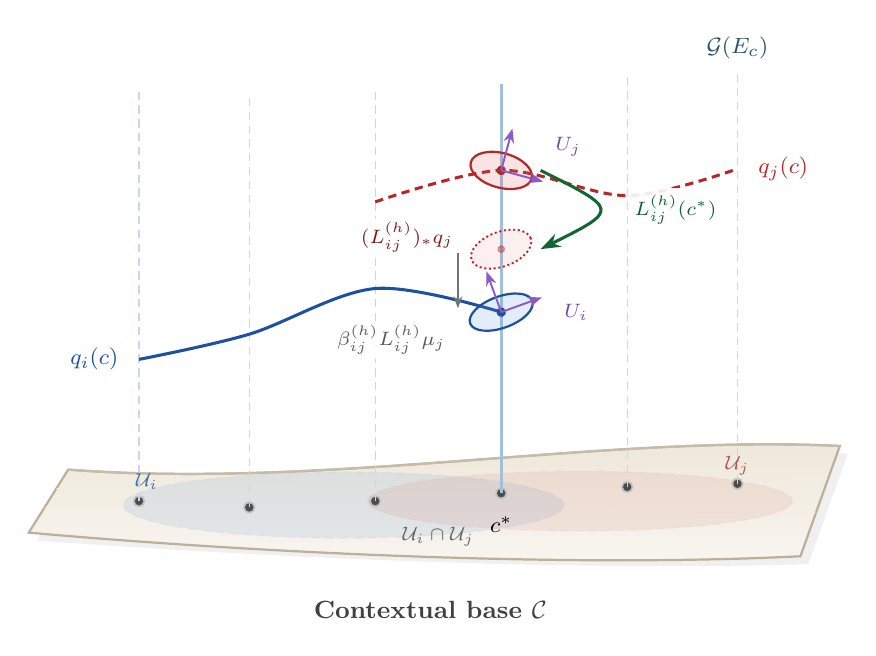
\begin{tikzpicture}[ every node/.style={font=\small}]

\definecolor{fiberblue}{RGB}{70,130,180}
\definecolor{sectionblue}{RGB}{30,80,160}
\definecolor{sectionred}{RGB}{180,40,40}
\definecolor{transportgreen}{RGB}{20,120,60}
\definecolor{gaussblue}{RGB}{100,150,220}
\definecolor{gaussred}{RGB}{220,100,100}
\definecolor{framecol}{RGB}{140,90,200}
\definecolor{basetan}{RGB}{230,220,200}
\definecolor{baseedge}{RGB}{160,140,110}
\definecolor{neighborblue}{RGB}{80,140,210}
\definecolor{neighborred}{RGB}{210,110,100}

\path
  (-0.3,0.1) coordinate (M1)
  (9.5,0.4) coordinate (M2)
  (9.0,-1.0) coordinate (M3)
  (-0.8,-0.7) coordinate (M4);

\filldraw[fill=black!6, draw=none]
  ($(M1)+(0.1,-0.1)$)
  .. controls (3.0,-0.2) and (6.5,0.6) .. ($(M2)+(0.1,-0.1)$)
  -- ($(M3)+(0.1,-0.1)$)
  .. controls (6.0,-1.2) and (2.0,-1.0) .. ($(M4)+(0.1,-0.1)$)
  -- cycle;

\shade[top color=basetan!70, bottom color=basetan!25, draw=baseedge!70, thick]
  (M1)
  .. controls (3.0,-0.15) and (6.5,0.55) .. (M2)
  -- (M3)
  .. controls (6.0,-1.15) and (2.0,-0.95) .. (M4)
  -- cycle;

\draw[baseedge!60, thick]
  (M1) .. controls (3.0,-0.15) and (6.5,0.55) .. (M2);

\foreach \t in {0.3, 0.6} {
  \draw[baseedge!15, very thin]
  ($(M1)!\t!(M4)$) .. controls
  ($($(M1)!\t!(M4)$)!0.4!($(M2)!\t!(M3)$)+(0,0.04)$) and
  ($($(M1)!\t!(M4)$)!0.6!($(M2)!\t!(M3)$)+(-0.02,-0.04)$)
  .. ($(M2)!\t!(M3)$);
}

\node[below, black!75, font=\small\bfseries] at (4.3,-1.45) {Contextual base $\mathcal{C}$};

\coordinate (C1) at (0.6,-0.30);
\coordinate (C2) at (2.0,-0.38);
\coordinate (C3) at (3.6,-0.30);
\coordinate (C4) at (5.2,-0.20);
\coordinate (C5) at (6.8,-0.12);
\coordinate (C6) at (8.2,-0.08);


\filldraw[neighborblue, opacity=0.12, draw=neighborblue!60,
  line width=0.5pt, densely dashed]
  (3.2,-0.35) ellipse (2.8 and 0.42);
\node[neighborblue!80!black, font=\scriptsize] at (0.7,-0.05) {$\mathcal{U}_i$};

\filldraw[neighborred, opacity=0.12, draw=neighborred!60,
  line width=0.5pt, densely dashed]
  (6.2,-0.30) ellipse (2.7 and 0.38);
\node[neighborred!80!black, font=\scriptsize] at (8.2,0.15) {$\mathcal{U}_j$};

\node[black!60, font=\scriptsize] at (4.4,-0.75) {$\mathcal{U}_i \cap \mathcal{U}_j$};

\foreach \c in {C1,C2,C3,C4,C5,C6} {
  \filldraw[black!25] (\c) circle (2pt);
  \filldraw[black!70] (\c) circle (1.3pt);
}

\pgfmathsetmacro{\fh}{5.2}

\foreach \c in {C1,C2,C3,C4,C5,C6} {
  \draw[fiberblue!30, densely dashed, line width=0.4pt]
  (\c) -- ++(0,\fh);
}

\node[above=2pt, fiberblue!60!black, font=\footnotesize]
  at ($(C6)+(0,\fh)$) {$\mathcal{G}(E_c)$};


\coordinate (Si1) at ($(C1)+(0,1.8)$);
\coordinate (Si2) at ($(C2)+(0,2.2)$);
\coordinate (Si3) at ($(C3)+(0,2.7)$);
\coordinate (Si4) at ($(C4)+(0,2.3)$);

\draw[sectionblue, line width=1.1pt]
  plot[smooth, tension=0.55] coordinates {
  (Si1) (Si2) (Si3) (Si4)
  };

\coordinate (Sj3) at ($(C3)+(0,3.8)$);
\coordinate (Sj4) at ($(C4)+(0,4.1)$);
\coordinate (Sj5) at ($(C5)+(0,3.7)$);
\coordinate (Sj6) at ($(C6)+(0,4.0)$);

\draw[sectionred, densely dashed, line width=1.1pt]
  plot[smooth, tension=0.55] coordinates {
  (Sj3) (Sj4) (Sj5) (Sj6)
  };

\node[sectionblue, font=\footnotesize, left=4pt] at (Si1) {$q_i(c)$};
\node[sectionred, font=\footnotesize, right=4pt] at (Sj6) {$q_j(c)$};


\draw[fiberblue!50, line width=1.0pt] (C4) -- ++(0,\fh);

\node[below=5pt, black, font=\footnotesize\itshape] at (C4) {$c^*$};


\begin{scope}[shift={(Si4)}, rotate=20]
  \filldraw[gaussblue, opacity=0.18] (0,0) ellipse (0.42 and 0.20);
  \draw[sectionblue, line width=0.8pt] (0,0) ellipse (0.42 and 0.20);
  \filldraw[sectionblue] (0,0) circle (1.5pt);
\end{scope}

\begin{scope}[shift={(Sj4)}, rotate=-15]
  \filldraw[gaussred, opacity=0.18] (0,0) ellipse (0.40 and 0.22);
  \draw[sectionred, line width=0.8pt] (0,0) ellipse (0.40 and 0.22);
  \filldraw[sectionred] (0,0) circle (1.5pt);
\end{scope}


\begin{scope}[shift={(Si4)}, rotate=20]
  \draw[-{Stealth[length=1.8mm]}, framecol, line width=0.7pt]
  (0,0) -- (0.55,0);
  \draw[-{Stealth[length=1.8mm]}, framecol, line width=0.7pt]
  (0,0) -- (0,0.55);
\end{scope}
\node[framecol!80!black, font=\scriptsize] at ($(Si4)+(0.95,0.0)$) {$U_i$};

\begin{scope}[shift={(Sj4)}, rotate=-15]
  \draw[-{Stealth[length=1.8mm]}, framecol, line width=0.7pt]
  (0,0) -- (0.55,0);
  \draw[-{Stealth[length=1.8mm]}, framecol, line width=0.7pt]
  (0,0) -- (0,0.55);
\end{scope}
\node[framecol!80!black, font=\scriptsize] at ($(Sj4)+(0.85,0.30)$) {$U_j$};


\coordinate (Ghost) at ($(Si4)+(0,0.8)$);
\begin{scope}[shift={(Ghost)}, rotate=20]
  \filldraw[gaussred, opacity=0.10] (0,0) ellipse (0.40 and 0.22);
  \draw[sectionred, densely dotted, line width=0.7pt] (0,0) ellipse (0.40 and 0.22);
  \filldraw[sectionred, opacity=0.4] (0,0) circle (1.2pt);
\end{scope}

\node[sectionred!70!black, font=\scriptsize,
  fill=white, fill opacity=0.9, text opacity=1,
  inner sep=1.5pt, rounded corners=1pt, anchor=east]
  (pushforwardlabel) at ($(Ghost)+(-0.55,0.15)$) {$(L_{ij}^{(h)})_*q_j$};

\draw[-{Stealth[length=2.5mm, width=1.8mm]},
  transportgreen!85!black, line width=1.1pt]
  ($(Sj4)+(0.5,0)$)
  .. controls ($(Sj4)+(1.5,-0.5)$) and ($(Ghost)+(1.5,0.5)$)
  .. ($(Ghost)+(0.5,0)$);

\node[transportgreen!80!black, font=\scriptsize\bfseries,
  fill=white, fill opacity=0.9, text opacity=1,
  inner sep=2.5pt, rounded corners=2pt, anchor=west]
  at ($(Sj4)!0.5!(Ghost)+(1.6,0)$) {$L_{ij}^{(h)}(c^*)$};


\draw[-{Stealth[length=1.5mm]},
  black!55, line width=0.6pt]
  ($(Ghost)+(-0.55,-0.05)$) -- ($(Si4)+(-0.55,0.05)$);

\node[black!65, font=\scriptsize,
  fill=white, fill opacity=0.9, text opacity=1,
  inner sep=1.5pt, rounded corners=1pt, anchor=east]
  (messagelabel) at ($(Si4)+(-0.65,-0.35)$) {$\beta_{ij}^{(h)}L_{ij}^{(h)}\mu_j$};

\end{tikzpicture}
}
\caption{\textbf{Local Gaussian sections and directed communication links.}
The curved surface represents the contextual base of the principal bundle; the curves are sections of its associated Gaussian-state bundle over overlapping neighborhoods. At a shared context \(c^*\), the local frames accompany the state glyphs. For one communication head indexed by \(h\), the green arrow applies \(L_{ij}^{(h)}=U_i\widetilde O_hT_hU_j^{-1}\) to the sender. The dotted contour depicts its Gaussian pushforward; the gray arrow identifies the weighted mean contribution to the receiver. A full-rank link is illustrated; a lower-rank link may produce a singular pushforward. The receiver's state need not equal that pushforward. Routing uses the separate comparison channel in Figure~\ref{fig:comparison_content_interfaces}. The finite token construction requires no smooth contextual base.}
\label{fig:link_construction}
\end{figure}

The geometric construction begins with a principal bundle of reference frames over a space of contexts. Let \(\mathcal C\) be a smooth contextual base and take \(G=\mathrm{GL}(K,\mathbb R)\). A principal bundle
\begin{equation}
\pi:\mathcal P\longrightarrow\mathcal C
\label{eq:principal_bundle}
\end{equation}
carries a free right action \(n\mapsto n\cdot g\) that preserves \(\pi\) and is transitive on each fiber. Locally, \(\mathcal P|_{\mathcal U}\simeq\mathcal U\times G\), with the group acting on the second factor. Thus a principal fiber consists of frame choices; choosing one frame identifies the fiber with \(G\). The probabilistic states are attached to this principal structure through associated bundles \citep{nakahara2003geometry,frankel2011geometry}.

Let \(\mathsf V=\mathbb R^K\) carry the defining representation of \(G\), and let
\begin{equation}
\mathcal B=\{\mathcal N(\mu,\Sigma):\mu\in\mathsf V,\ \Sigma\succ0\},
\qquad
\rho(g)\mathcal N(\mu,\Sigma)=\mathcal N(g\mu,g\Sigma g^\top).
\label{eq:gaussian_associated_action}
\end{equation}
The vector and Gaussian statistical bundles are
\begin{equation}
E=\mathcal P\times_G\mathsf V,
\qquad
\mathcal G(E)=\mathcal P\times_\rho\mathcal B.
\label{eq:associated_state_bundles}
\end{equation}
For the statistical bundle, the quotient convention is
\begin{equation}
(n\cdot g,b)\sim(n,\rho(g)b).
\label{eq:associated_quotient}
\end{equation}
Equivalently, \((n,b)\) and \((n\cdot g,\rho(g^{-1})b)\) represent the same associated point. The analogous relation uses \(v\mapsto gv\) for the vector bundle. The principal bundle carries gauge freedom, the vector bundle carries latent values, and the associated statistical bundle carries distributions over those values.

An agent over a contextual region \(\mathcal U_i\) selects a local principal section \(u_i\) and maintains belief and prior sections:
\begin{equation}
\begin{aligned}
u_i&:\mathcal U_i\longrightarrow\mathcal P,
&\pi\circ u_i&=\operatorname{id}_{\mathcal U_i},\\
q_i,p_i&\in\Gamma\bigl(\mathcal G(E)|_{\mathcal U_i}\bigr).
\end{aligned}
\label{eq:agent_bundle_sections}
\end{equation}
Here \(\Gamma\) denotes smooth sections, and the belief and prior have coordinates \((\mu_i,\Sigma_i)\) and \((\mu_{p,i},\Sigma_{p,i})\) in the section \(u_i\). Communication additionally uses one reference trivialization \(\sigma_0\) of \(\mathcal P\) on its working domain. The frame field is the relative element \(U_i\) defined by \(u_i=\sigma_0\cdot U_i^{-1}\), so that \(\xi_i=U_i^{-1}\mu_i\) are the \(\sigma_0\)-coordinates of the same vector. Identifying the fiber with its coordinates in the section \(u_i\), written \(E_c\), the frame is the linear isomorphism \(U_i(c):\mathsf V\to E_c\) that converts \(\sigma_0\)-coordinates into \(u_i\)-coordinates. On overlaps, agents can maintain different Gaussian sections at the same context. They are not required to be local representatives of one common belief. Figure~\ref{fig:link_construction} illustrates these associated statistical sections and their local frames. The attention construction uses this belief/prior sector; it does not require an additional bundle of generative-model parameters.

For token attention, the contextual dependence is evaluated at a fixed context \(c_0\), while \(i\in\mathcal I=\{0,\ldots,N-1\}\) labels the token agents. Keeping a separately labeled copy of the fiber for each token is the pullback along the constant map \(\iota:\mathcal I\to\mathcal C\), \(\iota(i)=c_0\):
\begin{equation}
\mathcal P_{\mathcal I}=\iota^*\mathcal P,
\qquad E_{\mathcal I}=\iota^*E.
\label{eq:token_bundle_pullback}
\end{equation}
Write \(E_i\) for the vector fiber at token \(i\). This notation distinguishes token incidence from the contextual base of the general construction. Because \(\iota\) is constant, \(\iota^*\mathcal P=\mathcal I\times\mathcal P_{c_0}\) canonically. The token construction therefore sees no connection, curvature, or topology of \(\mathcal P\), and its gauge group is \(G^N\), on which the contextual gauge group acts only through the diagonal. Placing tokens at distinct contexts \(\iota(i)=c_i\) and realizing links by parallel transport along declared base curves would make the contextual connection enter the attention operator. The section of each token agent and the reference trivialization give \(U_i:\mathsf V\to E_i\), and its statistical fiber is
\begin{equation}
\mathcal G(E_i)=\{\mathcal N(\mu,\Sigma):\mu\in E_i,\ \Sigma\succ0\}.
\label{eq:overview_statistical_fiber}
\end{equation}
A general contextual principal bundle need not admit a global section. The factorized attention formulas use the reference trivialization \(\sigma_0\) on their working domain; on the finite token pullback this trivialization is canonical. The communication graph is additional data; the matrix links on it are determined by the frames, the shared interfaces, and the routing weights. A link \(L_{ij}:E_j\to E_i\) can be singular, so it is not in general a principal-bundle transition function or a group-valued parallel transport. Sections~\ref{sec:construction_overview} and~\ref{sec:matrix_link_fields} construct these links from comparison and content interfaces while retaining the underlying principal-bundle structure.

\section{Irreducible Frame Blocks and Communication Heads}
\label{sec:heads_irreps}

The representation carried by a state and the organization of its communication heads are separate structures. To make their relationship precise, fix a decomposition $\mathsf V=\bigoplus_{b=1}^{B}\mathsf V_b$, with $\mathsf V_b\simeq\mathbb R^{d_b}$ and $K=\sum_bd_b$, and restrict the frame group to
\begin{equation}
G=\prod_{b=1}^{B}\mathrm{GL}(d_b,\mathbb R),\qquad
\rho(g_1,\ldots,g_B)=\bigoplus_{b=1}^{B}g_b,\qquad
U_i=\bigoplus_{b=1}^{B}U_i^{(b)}.
\label{eq:frame_product_representation}
\end{equation}
Here $B$ counts independently transforming frame blocks, while $H$ counts communication heads. Each $\mathsf V_b$ is an irreducible real representation of $G$: a nonzero invariant subspace contains the orbit of any one of its nonzero vectors, and the $b$th general linear factor maps that vector to every other nonzero vector in $\mathsf V_b$. Thus no proper nonzero invariant subspace exists. These representations remain inequivalent when their dimensions coincide, because the product factors act independently. Repeating the same group element on several blocks would instead give equivalent copies of one representation. Equation~\eqref{eq:frame_product_representation} is an explicit specialization of the full $\mathrm{GL}(K)$ action, not a theorem that an arbitrary attention architecture has this decomposition.

In this appendix $O_h$ denotes the applied receiving map, written $\widetilde O_h$ in the main text; in the affine chart the two coincide. Let $\operatorname{pr}_b:\mathsf V\to\mathsf V_b$ and $\iota_b:\mathsf V_b\to\mathsf V$ be the coordinate projection and inclusion, and put $E_i^{(b)}=U_i\mathsf V_b$. A head $h$ is local to a block $b=b(h)$ when its interface maps factor as
\begin{equation}
S_{Q,h}=\overline S_{Q,h}\operatorname{pr}_b,\quad
S_{K,h}=\overline S_{K,h}\operatorname{pr}_b,\quad
T_h=\overline T_h\operatorname{pr}_b,\quad
O_h=\iota_b\overline O_h.
\label{eq:block_local_head_conditions}
\end{equation}
The barred maps act on the selected block; the comparison maps retain the full-row-rank requirement. The resulting $L_{ij}^{(h)}=U_i\iota_b\overline O_h\overline T_h\operatorname{pr}_bU_j^{-1}$ communicates only between the corresponding site subspaces $E_j^{(b)}$ and $E_i^{(b)}$. Taking $H=B$ and a one-to-one assignment gives a precise sense in which heads can be organized by irreducible blocks. The irreducible object is the vector carrier $E_i^{(b)}$, however, not the Gaussian density or the entire attention operation. The common reference channels remain fixed under the passive site action of Eq.~\eqref{eq:passive_site_action}. A proper selected row space inside the carrier is not invariant under the full defining $\mathrm{GL}(d_b)$ action. In the full-input/output construction, $S_Q,S_K,T,O$ need not satisfy Eq.~\eqref{eq:block_local_head_conditions}; a head can access several blocks. Its endpoint covariance follows from the transforming frames, without requiring the fixed reference maps to be group intertwiners.

Independent Gaussian blocks require an additional statistical assumption. If every local covariance is block diagonal, $\Sigma_i=\bigoplus_b\Sigma_i^{(b)}$, then the full Gaussian laws factor and block-diagonal reference transport gives
\begin{equation}
D_{\mathrm{KL}}\bigl(q_i\|(\Omega_{ij})_*q_j\bigr)
=\sum_{b=1}^{B}D_{\mathrm{KL}}\bigl(q_i^{(b)}\|(\Omega_{ij}^{(b)})_*q_j^{(b)}\bigr),
\quad \Omega_{ij}^{(b)}=U_i^{(b)}(U_j^{(b)})^{-1}.
\label{eq:irrep_block_kl_additivity}
\end{equation}
Here $q_i^{(b)}$ is the block marginal. The identity follows by writing the logarithm of the product-density ratio as a sum and integrating each normalized factor \citep[Thm.~28]{vanErvenHarremoes2014}. Block-diagonal frames alone do not imply it. For example, $q=\mathcal N(0,\left(\begin{smallmatrix}1&c\\c&1\end{smallmatrix}\right))$, $p=\mathcal N(0,I_2)$, and $0<|c|<1$ have identical one-dimensional marginals but $D_{\mathrm{KL}}(q\|p)=-\tfrac12\log(1-c^2)>0$. Furthermore, separate routing distributions for the blocks are a modeling choice: softmax of the summed KL chooses one shared source and does not equal independent headwise source selection.

The frame generators have a related but different decomposition. At a block, $\mathfrak{gl}(d_b)=\mathfrak{sl}(d_b)\oplus\mathbb RI_{d_b}$ separates traceless generators from the central dilation generator; it is not a decomposition of the state space into two irreducible heads. At the ambient level,
\begin{equation}
\mathfrak{gl}(K)=\left(\bigoplus_b\mathfrak{gl}(d_b)\right)
\oplus_{\mathrm{vec}}\mathfrak m,\qquad
\mathfrak m=\bigoplus_{b\ne c}\operatorname{Hom}(\mathsf V_c,\mathsf V_b),\qquad
\dim\mathfrak m=K^2-\sum_bd_b^2.
\label{eq:off_block_vector_complement}
\end{equation}
The subscript emphasizes a vector-space splitting. The off-block complement is preserved by block-diagonal conjugation but is generally not a Lie subalgebra: for two scalar blocks, $[E_{12},E_{21}]=E_{11}-E_{22}$ is block diagonal. Restoring these generators enlarges the frame group; it does not add the only possible cross-block communication, since full-width interface maps already provide such communication.

Representation-based attention has established precedents. The SE(3)-Transformer uses irreducible rotation types with invariant attention and equivariant values; its multi-head construction partitions multiplicity channels while retaining several representation types in each head \citep[Secs.~2.3 and 3.2, App.~D.3]{fuchs2020se3}. Gauge Equivariant Transformer combines local-frame-equivariant multi-head attention with regular fields and their irreducible decomposition \citep[Secs.~4.1--4.2]{He2021GaugeEquivariantTransformer}. The subject here is the particular combination of full Gaussian comparison laws, separately specified sending/receiving interfaces, and the matrix links $U_iO_hT_hU_j^{-1}$. The frame blocks specify the state representation, while the comparison and content interfaces specify how that state is used for communication.


\section{Positional and Masking Priors}
\label{sec:nonuniform_priors}

With a nonuniform prior, Eq.~\eqref{eq:mixture_softmax_general} adds $\log\pi_{ij}$ to the logits with unit coefficient while the cost is divided by $\tau$, so temperature never rescales a positional preference. Masks and positional biases therefore enter as priors over sources. This identification, and the entropy-regularized or transport form of the softmax that underlies it, is established in the attention literature \citep{Niculae2017Regularized,Litman2025EOT,Bianchessi2026BAM,Litman2026AttentionPriors}. On the causal support $S_i=\{0,\ldots,i\}$, the uniform prior $\pi_{ij}=\mathbf{1}[j\le i]/(i+1)$ gives the support and row normalization of GPT-family attention \citep{radford2019language}. A window of radius $w$, $\pi_{ij}\propto\mathbf{1}[i-w\le j\le i]$, gives the sliding-window support of Longformer and Mistral \citep{beltagy2020longformer,jiang2023mistral}. The prior $\pi_{ij}\propto\exp[-\alpha_h(i-j)]$ gives the linear biases of attention with linear biases (ALiBi) \citep{press2022train}, and $\log\pi_{ij}=f_h(i-j)+\mathrm{const}$ gives learned relative biases, parameterized by sinusoids in the global positional bias of Transformer-XL and shared within logarithmic offset buckets in T5 \citep{dai2019transformerxl,raffel2020exploring}. \citet{press2022train} state the geometric slope schedule $\alpha_h=2^{-8h/H}$; their reference implementation uses it when $H$ is a power of two and otherwise appends alternate slopes of the next power-of-two schedule. The construction fixes only the form in which a prior enters. It does not select a prior, except that the autoregressive factorization requires $\pi_{ik}=0$ for $k>i$ at every layer, because each state depends on its own token.


\section{An Optional Prior-Bank Vocabulary Readout}
\label{sec:prior_bank_readout}

Let $q_i$ be the Gaussian state after the chosen forward computation and $p_v$ a normalized class template on the same latent space, with finite $D_{\mathrm{KL}}(q_i\|p_v)$. Declaring the templates in reference coordinates and comparing them with $\widetilde q_i=(U_i^{-1})_*q_i$ makes the readout invariant under the passive action; comparing local coordinates directly defines a different, non-covariant readout. No convergence of $q_i$ is assumed. Specify a categorical readout $\hat p_i$ by minimizing
\begin{equation}
\mathcal J_{\mathrm{decode}}(\hat p_i)
=\sum_v\hat p_i(v)D_{\mathrm{KL}}(q_i\|p_v)
+\tau_{\mathrm{dec}}D_{\mathrm{KL}}(\hat p_i\|\omega),
\qquad\tau_{\mathrm{dec}}>0,
\end{equation}
where $\omega$ is a class prior. The unique optimum on its support is
\begin{equation}
\hat p_i(v)\propto\omega_v\exp\left[-D_{\mathrm{KL}}(q_i\|p_v)/\tau_{\mathrm{dec}}\right].
\label{eq:readout_gibbs}
\end{equation}
This is a specified Gibbs readout. At unit temperature it is also the categorical mean-field coordinate update for a fixed $q_i$ under the normalized mixture $p(v,x)=\omega_vp_v(x)$, as in the general expected-log update of \citet[\S2.4, Eqs.~17--18]{Blei2017}. It is not generically the posterior-predictive average of a classifier.

The score identity is exact:
\begin{equation}
\mathbb E_{q_i}[\log p_v(X)]
=-D_{\mathrm{KL}}(q_i\|p_v)-H(q_i).
\label{eq:readout_kl_decomposition}
\end{equation}
The entropy is independent of $v$ and cancels in the categorical softmax. For Gaussian $q_i=\mathcal N(\mu_i,\Sigma_i)$ and $p_v=\mathcal N(\mu_{p,v},\Sigma_{p,v})$, the expectation is
\begin{equation}
-\frac12\left[
\operatorname{Tr}(\Sigma_{p,v}^{-1}\Sigma_i)
+(\mu_i-\mu_{p,v})^\top\Sigma_{p,v}^{-1}(\mu_i-\mu_{p,v})
+\log\det\Sigma_{p,v}+K\log(2\pi)
\right].
\label{eq:readout_expected_loglik}
\end{equation}
These are Gaussian cross-entropy identities \citep{Bishop2006}.

For the normalized point classifier
\begin{equation}
p(v\mid x)=\frac{\omega_vp_v(x)}
{\sum_w\omega_wp_w(x)},
\label{eq:readout_point_classifier}
\end{equation}
posterior prediction instead averages probabilities,
$\bar p_i(v)=\mathbb E_{q_i}[p(v\mid X)]$. This generally differs from normalizing $\exp(\mathbb E_{q_i}\log p(v\mid X))$. For example, with equal class priors, $q_i=\mathcal N(0,4)$ and templates $p_0=\mathcal N(0,1)$, $p_1=\mathcal N(2,1)$, the unit-temperature Gibbs readout is $\hat p_i(1)=1/(1+e^2)\approx0.11920$. The predictive average is
\begin{equation}
\bar p_i(1)=\mathbb E_{X\sim\mathcal N(0,4)}
\left[\frac{1}{1+\exp(2-2X)}\right]\approx0.32383.
\end{equation}
The expected-log construction therefore does not replace the predictive integral. Both readouts are variational: among joints whose latent marginal is fixed to $q_i$, the unrestricted minimizer of the KL to $\omega_vp_v(x)$ has class marginal $\bar p_i$, and the minimizer within the product family is the Gibbs readout. The same distinction separates the Gibbs routing row from the posterior-predictive source probability of Section~\ref{sec:exact_posterior}.

Uniform $\omega$ gives logits $-D_{\mathrm{KL}}(q_i\|p_v)/\tau_{\mathrm{dec}}$. Projecting a full-covariance belief before decoding makes this identity exact for the projected distribution only. Choosing a temperature or learning an additional scalar is a modeling choice. Cross-entropy training of this readout does not become optimization of the full belief free energy merely because its scores are divergences. The linear decoder used in the experiment of Section~\ref{sec:lm_realization} is itself the unit-temperature Gibbs readout for the shared-covariance templates $p_v=\mathcal N(\Sigma_*w_v,\Sigma_*)$, with $w_v$ the $v$th row of $W_{\mathrm{out}}$ and class prior $\log\omega_v=b_{\mathrm{out},v}+\kappa_{\mathrm{uni}}\log p_{\mathrm{uni}}(v)+\tfrac12w_v^\top\Sigma_*w_v$ up to a constant, for any $\Sigma_*\succ0$; the belief covariance cancels from every logit difference. The token-bank readout differs by giving each class its own template covariance.

\section{Relation to a Normalized Latent-Source Model}
\label{app:fixed_joint_bridge}

A broader gauge-theoretic variational free energy (VFE) theory begins with a normalized generative law and a separately specified population recognition law. Geometry alone supplies neither. Let $z$ collect the declared agent and auxiliary latent variables (the latent configuration, written $y$ in the broader theory), let $X$ denote fixed structural data, and let each record kernel have a normalized density $\ell_a$. A normalized latent law $p_\theta^Z$, constructed for example by finite directed kernel composition, gives
\begin{equation}
p_\theta(z,o\mid X)=p_\theta^Z(z\mid X)\prod_a\ell_a(o_a\mid z_{\partial a},X).
\label{eq:rg_bridge_joint}
\end{equation}
Integrating the records first leaves the unit mass of $p_\theta^Z$. Record scopes may overlap because each record is a conditional output of the same latent configuration. The factors are fixed while recognition varies. Latent variables may themselves take values in a space of probability laws; this does not permit a generative factor to read the recognition distribution being optimized.

Fix a regular observation slice with $0<p_\theta(o\mid X)<\infty$. Let $Q$ have density $q$, satisfy $Q\ll P_\theta(\cdot\mid o,X)$, and have finite expectations of $|\log q|$ and $|\log p_\theta(z,o\mid X)|$. Defining $\mathcal L_\theta(Q)=\mathbb E_Q[\log p_\theta(z,o\mid X)-\log q(z)]$ gives
\begin{equation}
\log p_\theta(o\mid X)=\mathcal L_\theta(Q)+D_{\mathrm{KL}}\bigl(Q\|P_\theta(\cdot\mid o,X)\bigr).
\label{eq:rg_bridge_elbo}
\end{equation}
Indeed, Bayes' formula makes the log density ratio equal to $\log q-\log p_\theta(z,o\mid X)+\log p_\theta(o\mid X)$; integrating proves the identity. The KL is nonnegative and vanishes exactly at equality of the full laws. No factorization of $Q$ is assumed. Outside the finite-density domain, the extended free energy is defined as $-\log p_\theta(o\mid X)+D_{\mathrm{KL}}(Q\|P_\theta(\cdot\mid o,X))$, avoiding undefined differences of infinite expectations. This is the standard evidence-bound construction \citep[Sec.~2.2, Eq.~14]{Blei2017}; consistent passive pushforwards preserve its relative entropy.

The broader theory also supplies a route to categorical attention. Give each receiver-head pair $(i,h)$ an independent source label $J_i^{(h)}$ with prior $\pi_i^{(h)}$ and a binary compatibility record $\chi_i^{(h)}\in\{0,1\}$, and take
\begin{equation}
\begin{aligned}
p_\theta(z,j,\chi,o\mid X)={}&p_\theta^Z(z\mid X)\prod_{i,h}\pi_i^{(h)}\bigl(j_i^{(h)}\bigr)\operatorname{Bern}\Bigl(\chi_i^{(h)};\exp\bigl[-D_{ij_i^{(h)}}^{(h)}(z)/\tau_h\bigr]\Bigr)\\
&\times\prod_a\ell_a(o_a\mid z_{\partial a},X),
\end{aligned}
\label{eq:rg_bridge_record_joint}
\end{equation}
in which no other factor reads a label. Each record kernel is normalized for every $\tau_h>0$ because $D_{ij}^{(h)}\ge0$; for a cost that is only finite, replacing $D$ by $D-\min_kD_{ik}$ multiplies the selected-record likelihood by a label-independent factor. Conditioning on $\chi=\mathbf 1$ gives the exact conditional rows $P(J_i^{(h)}=j\mid z,\chi,o)=\operatorname{softmax}_j\bigl(\log\pi_{ij}^{(h)}-D_{ij}^{(h)}(z)/\tau_h\bigr)$, independent across $(i,h)$. This is the optimality-variable device of control as inference \citep{Levine2018}. Under $Q(dz,dj)=Q_Z(dz)\prod_{i,h}\beta_i^{(h)}(dj_i^{(h)})$ with $\mathbb E_{Q_Z}|D_{ij}^{(h)}|<\infty$, the row-dependent free energy and its optimizer are
\begin{align}
\mathcal F_i^{(h)}(\beta_i^{(h)})&=D_{\mathrm{KL}}(\beta_i^{(h)}\|\pi_i^{(h)})+\tau_h^{-1}\sum_j\beta_{ij}^{(h)}\mathbb E_{Q_Z}D_{ij}^{(h)},\\
\beta_{ij}^{(h)*}&=\operatorname{softmax}_j\bigl(\log\pi_{ij}^{(h)}-\mathbb E_{Q_Z}D_{ij}^{(h)}/\tau_h\bigr).
\label{eq:rg_bridge_row}
\end{align}
Expansion of the factorized density gives the first expression up to a row-independent term; a normalization multiplier gives the second. The pointwise generative posterior instead uses $D_{ij}^{(h)}(z)$ inside softmax. Multiplying a row objective by $\tau_h$ preserves its optimizer, but does not license independently rescaling sectors of one global evidence lower bound (ELBO).

The fixed-context Gaussian mixture of Section~\ref{sec:mixture_derivation} supplies a different local joint with the same unit-temperature row objective: at unit temperature its KL is the projected Gaussian comparison cost plus categorical relative entropy. Appending the same normalized content law in the model and recognition factors makes that content law cancel, as in Eq.~\eqref{eq:relational_normalized_model}. It therefore permits the chosen message means without deriving the learned content maps or residual. The general Gaussian realization likewise permits singular conditional mean maps with positive-definite receiving noise, but that normalization fact does not select the predictive attention architecture.

The autoregressive softmax predictor already defines a normalized probability law, and its outer cross-entropy is the corresponding negative log-likelihood; in evaluation each conditional is computed from a bounded window, which leaves every factor normalized. For the attention sublayer, a normalized latent model exists in which routing is the exact label posterior and the content-plus-residual update is the exact predictive mean (Theorem~\ref{thm:probabilistic_status}). What remains unresolved is a latent joint and recognition construction that also covers the normalization and MLP maps, the collapse of the predictive mixture to a point state between layers, and the relation of cross-entropy training to that model's evidence. A model with no latent variables would make the evidence identity tautological without deriving those operations.


\section{Additional Scope Results for Gaussian Predictive Architectures}
\label{app:architecture_scope}

The main text distinguishes geometric attention from a complete model of population inference and nonlinear state evolution. The following calculations state the population-covariance, Gaussian-closure, and causal-prediction conditions used in the main text. They concern the declared states and predictive maps.

\subsection{Population covariance and link-residual costs}
\label{sec:population_link_residuals}

Let a joint population state have law
\(\mathcal N(\boldsymbol\mu,\Gamma)\), with covariance blocks
\(\Gamma_{ij}=\operatorname{Cov}(k_i,k_j)\) and
\(\Gamma_{ii}=\Sigma_i\). For a fixed link \(L_{ij}:E_j\to E_i\), set
\(e_{ij}=k_i-L_{ij}k_j\) and
\(\bar e_{ij}=\mu_i-L_{ij}\mu_j\). Bilinearity of covariance gives
\begin{equation}
V_{ij}:=\operatorname{Cov}(e_{ij})
=\Sigma_i+L_{ij}\Sigma_jL_{ij}^{\top}
-\Gamma_{ij}L_{ij}^{\top}-L_{ij}\Gamma_{ji}.
\label{eq:population_residual_covariance}
\end{equation}
This identity needs no inverse of \(L_{ij}\). For any receiving covariance \(R_i\succ0\), expansion around the mean gives the expected quadratic cost
\begin{equation}
\mathbb E[e_{ij}^{\top}R_i^{-1}e_{ij}]
=\bar e_{ij}^{\top}R_i^{-1}\bar e_{ij}
+\operatorname{Tr}(R_i^{-1}V_{ij}).
\label{eq:population_residual_cost}
\end{equation}
The centered cross terms have zero expectation, leaving the trace term. These are Gaussian moment identities \citep{Bishop2006}; the two displayed moment formulas also hold for non-Gaussian laws with finite second moments.

A product approximation to the population sets the off-diagonal blocks \(\Gamma_{ij}\) to zero. Local state covariances alone do not justify that substitution. For a scalar example, take unit marginal variances, zero means, \(L_{ij}=1\), and cross covariance \(c\), with \(|c|<1\). The expected squared residual is \(2(1-c)\), while every individual Gaussian marginal is unchanged as \(c\) varies. Thus comparing local distributions and computing a correlated population residual are different operations.

A Gaussian record with mean \(k_i-L_{ij}k_j\) and positive-definite noise can use Eq.~\eqref{eq:population_residual_cost} inside a normalized population model of Appendix~\ref{app:fixed_joint_bridge}. Its expected log-likelihood cost is not generically the KL between the two projected Gaussian marginals in the main text. That KL has its own trace and determinant terms. Substituting a marginal divergence for the record cost changes the probabilistic model unless a separate identity establishes their equality.

\subsection{Nonlinear mean maps and full Gaussian laws}
\label{sec:nonlinear_gaussian_scope}

An operation on a Gaussian mean does not automatically specify the pushforward of its entire law. To see this for LayerNorm \citep{ba2016layernorm}, put \(P_0=I-\mathbf1\mathbf1^\top/K\) and define
\begin{equation}
\operatorname{LN}_\epsilon(x)
=\frac{P_0x}{\sqrt{\|P_0x\|^2/K+\epsilon}}.
\label{eq:layernorm_gaussian_scope}
\end{equation}
For \(K=2\), \(\epsilon=0\), and a nondegenerate Gaussian input, \(x_1=x_2\) has probability zero and
\begin{equation}
\operatorname{LN}_0(x)
=\operatorname{sign}(x_1-x_2)(1,-1).
\label{eq:layernorm_two_atoms}
\end{equation}
The output law has two atoms. For \(\epsilon>0\) and arbitrary \(K\ge2\), the output remains in the proper zero-sum hyperplane, and it is bounded, \(\|\operatorname{LN}_\epsilon(x)\|^2<K\), so its law is not even a degenerate Gaussian. Fixed affine gains and biases map this support into an affine subspace of dimension at most \(K-1\). Neither construction is a nondegenerate full Gaussian pushforward. Applying normalization only to \(\mu_i\), while retaining \(\Sigma_i\) for routing, remains a valid specified coordinate operation; it has a different statistical meaning.

\subsection{Prefix-based causal prediction}
\label{sec:causal_prediction_scope}

A predictive conditional requires a state determined only by the available prefix and shared across all candidate next tokens. If one separately recomputes a binary state after inspecting each candidate target and assigns that target probability \(3/4\), each row is normalized but the two candidate scores sum to \(3/2\). They are not one conditional probability law. By contrast, a single prefix-based state followed by one categorical readout defines a normalized kernel, and the product of such kernels defines a finite sequence law by successive summation. The main architecture uses this direct causal construction. Outer backpropagation from training targets updates shared parameters; it does not insert those targets into the prediction-time state.


\section{Numerical Identity Checks}
\label{app:identity_checks}

The identities of Sections~\ref{sec:lie_links}, \ref{sec:receiver_inference}, and~\ref{sec:lie_holonomy} were evaluated in float64 at small sizes with random inputs by the script \texttt{glk\_\allowbreak lie\_\allowbreak links\_\allowbreak checks/\allowbreak checks.py}, whose output accompanies it. The written derivations carry the mathematical claims; the checks test the formulas, and their sizes, $K\le7$ with at most three heads and four sources, carry no information about trained models or large networks. All $58$ checks passed.

The low-rank exponential of Lemma~\ref{lem:lie_lowrank} holds to a relative error of $8.5\times10^{-16}$, the augmented-exponential evaluation of $\varphi_1$ agrees with its series to $2.6\times10^{-15}$, and the split of Proposition~\ref{prop:lie_split} holds to $5.5\times10^{-16}$, with the identity on $\ker T_h$, the image condition, and the determinant identity at the level of rounding. The first-order defect $(\Theta_{ij}(s)-\Omega_{ij})/s-L_{ij}^{(h)}$ is $8.5\times10^{-3}$, $8.5\times10^{-4}$, and $8.5\times10^{-5}$ at $s=10^{-2}$, $10^{-3}$, and $10^{-4}$. The passive law and the adjoint action of a common reference change hold to $8\times10^{-16}$, and the numerical matrix logarithm of $\operatorname{diag}(-1,-2)$ is complex, as item 4 of Proposition~\ref{prop:lie_endpoint} requires. On the principal-logarithm domain the conversion of Proposition~\ref{prop:lie_charts} gives $TO=Z$ to $2.4\times10^{-15}$ and $\exp(OT)=I+O_{\mathrm{lin}}T$ to $1.6\times10^{-16}$, and the embedding $\Upsilon$ is a determinant-preserving homomorphism satisfying items 2 and 3 to $3\times10^{-15}$. The complement split of Lemma~\ref{lem:lie_complement} holds to $2.7\times10^{-14}$ at $K=7$ with $S=4$, and exact enumeration over head-label tuples reproduces Eq.~\eqref{eq:lie_aggregate} with a receiver-carried complement to $3.4\times10^{-16}$. In the tiled case the three forms of the resummed receiving map, the effective transfer $T\widetilde O=e^{TO}$, the head-sum identity, the projector relations of Proposition~\ref{prop:lie_order_zero}, and the order series of Eq.~\eqref{eq:lie_orders} hold to $2\times10^{-15}$; the second-order truncation vanishes exactly at the stated matrix, and $\sigma_{\min}(e^X)\ge e^{-\|X\|_2}$ held on $200$ random generators. The pinned latent-link transport reproduces the exponential-chart message of Remark~\ref{rem:lie_static_limit} to $2.4\times10^{-15}$.

For the holonomy, the triangle spectra of Proposition~\ref{prop:lie_triangle_spectrum} match those of $\boldsymbol\rho_{ijk}TO$ and $\boldsymbol\rho_{ijk}e^{TO}$ to $1.3\times10^{-14}$ with $TO\ne I$, the head-sum loop with $TO=I$ matches Table~\ref{tab:lie_holonomy} to $2\times10^{-15}$, and the flat identification has trivial holonomy. The errors of the first- and second-order truncations of Eq.~\eqref{eq:lie_bch} scale as the square and the cube of the generator scale. The flat routing pattern $c=(1,0.5,0.2,0.05,0.01)$ has positive rows summing to one and zero cocycle defect. All eigenvalue statistics vanish on the shear $I+E_{12}$ while its Frobenius defect is $\tfrac12$, the Frobenius defect is invariant under a multiple of an orthogonal matrix, and a non-conformal diagonal reparametrization changes it.

For the receiver, $200$ random perturbations do not lower the energy of Eq.~\eqref{eq:rec_channel_energy} below its value at the closed form of Proposition~\ref{prop:rec_closed_form}, central differences of the energy vanish there to $1.8\times10^{-9}$, the closed form equals the Gaussian power posterior to $9\times10^{-16}$, and $F-\lambda_\alpha D_{\mathrm{KL}}(q\|p_{\mathrm{pow}})$ is constant in $q$ to $5\times10^{-15}$. The unobserved marginal of item 3 of Corollary~\ref{cor:rec_properties} equals the prior marginal to $1.1\times10^{-15}$, the predictive limit of Proposition~\ref{prop:rec_predictive_limit} holds to $1.3\times10^{-9}$ at prior precision $10^{-10}$, the natural-parameter interpolation of Proposition~\ref{prop:rec_flow} agrees with a fourth-order Runge--Kutta integration of the Fisher flow to $6\times10^{-15}$, and the frozen energy decreases along the damped full-family update. The profiled per-coordinate majorize-minimize step never increased the profiled energy over $300$ random instances of four iterations each, the episode-start step equals the Kalman form of Eq.~\eqref{eq:rec_kalman}, the damped diagonal counterexample reproduces $1.500$, $2.503$, and $1.000$, and the local closed form is the frame image of the reference closed form. A Monte Carlo estimate from $4\times10^5$ draws matches the moment-matched covariance of Eq.~\eqref{eq:predictive_kernel_covariance} to a relative error of $2.3\times10^{-3}$ at $r=0$ and $2.0\times10^{-3}$ at $r=1$.

% PLACEHOLDER S: experimental record and diagnostics for the final runs.
\section{Experimental Record and Diagnostics}
\label{app:placeholder_experimental_record}

This appendix reserves the experimental record of the final runs. Each table and figure below is a placeholder to be replaced by recorded values or artwork. % PLACEHOLDER

\begin{table}[htbp]
\centering
\small
\begin{tabular}{p{0.30\linewidth}p{0.62\linewidth}}
\toprule
Reporting field & Final-run value or artifact identifier \\
\midrule
Source and configuration & pending: source archive and hash, configuration schema, resolved operator selectors \\
Data and tokenizer & pending: dataset and split revision, tokenizer and version, vocabulary, concatenation policy, token-cache hashes, unique training tokens, passes \\
Architecture & pending: $K$, blocks, heads, ranks $r_h,s_h$, depth, normalization placement, residual, MLP width, decoder \\
Initialization & pending: prior means and covariances, frame generators, interface maps, as executed \\
Optimization & pending: learning rate and weight decay for every parameter table, schedule, warmup, clipping groups, post-update frame projection \\
Numerical realization & pending: precision per operation, cost bound, reduced-covariance factorization and failure policy, matrix-exponential policy \\
Training budget & pending: token presentations, updates, batch and accumulation, device-hours \\
Evaluation & pending: checkpoint-selection rule, context, stride, scored targets, masking \\
\bottomrule
\end{tabular}
\caption{Reproducibility contract for the final reported runs. Populate each field from the executing source archive and its saved metadata, and separate effective settings from accepted but inactive selectors.}
\label{tab:placeholder_methods_contract}
\end{table}

\begin{table}[htbp]
\centering
\small
\begin{tabularx}{\linewidth}{@{}>{\raggedright\arraybackslash}Xcc@{}}
\toprule
Parameter role or resource & Evaluated run & Final run \\
\midrule
Per-type tables (token frames, prior means and covariances, decoder) & pending & pending \\
Positional frame generators & pending & pending \\
Context-processing parameters (interface maps, MLP, normalization) & pending & pending \\
Parameters read per token & pending & pending \\
Optimizer state and peak device memory & pending & pending \\
Training throughput and device-hours & pending & pending \\
Inference latency at declared batch and context & pending & pending \\
\bottomrule
\end{tabularx}
\caption{Reserved storage and cost record. Sparse access to per-type tables reduces the parameters read per token but not the stored parameters; report both, together with measured throughput under a declared precision.}
\label{tab:placeholder_resources}
\end{table}

\begin{table}[htbp]
\centering
\small
\begin{tabular}{lccccc}
\toprule
Model arm & Seeds & Selected step & Validation CE & Test CE & Test PPL \\
\midrule
pending & pending & pending & pending & pending & pending \\
\bottomrule
\end{tabular}
\caption{Reserved per-seed results for every arm of the main results table. List the model seed and the data-order seed, and apply the checkpoint-selection rule identically across arms.}
\label{tab:placeholder_per_seed}
\end{table}

\begin{table}[htbp]
\centering
\small
\begin{tabular}{lccc}
\toprule
Model and source & Tokenization & Context & Word-normalized test PPL \\
\midrule
Evaluated realization & GPT-2 BPE & pending & pending \\
Published reference points & pending & pending & pending \\
\bottomrule
\end{tabular}
\caption{Reserved calibration of the headline result. Word-normalized perplexity is the exponential of the summed test negative log-likelihood divided by the number of word-level test tokens, after an audit confirming that both token streams encode the same text. Published rows use different protocols and are contextual references, not matched comparisons.}
\label{tab:placeholder_calibration}
\end{table}

\begin{figure}[htbp]
\centering
\placeholderbox{66mm}{PLACEHOLDER S1\\[3mm]
Panel A: per layer, quantiles across tokens of the ratio $\|m_i\|/\|\mu_i\|$ of message to residual state, over training.\\[2mm]
Panel B: common scale and scale-free invariants of the comparison maps (relative gains and principal angles of $S_{Q,h},S_{K,h}$), and the largest singular value of $O_hT_h$, over training.\\[2mm]
Panel C: mean and spread of the stored log-variances over training, with the curve implied by weight decay alone.\\[2mm]
Panel D: counts, with denominators, of cost-bound activations, factorization fallbacks, frame-generator projections, and skipped updates.\\[2mm]
TO COLLECT: per-table norms and invariants at every evaluation, and instrumented event counters.}
\caption{Reserved training-dynamics and numerical diagnostics. The routing costs are unchanged when a common invertible map acts on $S_{Q,h}$ and $S_{K,h}$, and the messages are unchanged under $(T_h,O_h)\mapsto(BT_h,O_hB^{-1})$. Gradient flow conserves the corresponding quantities $S_{Q,h}S_{Q,h}^\top+S_{K,h}S_{K,h}^\top$ and $T_hT_h^\top-O_h^\top O_h$, whereas adaptive optimizers without weight decay move along these directions; Panel B therefore separates motion along the symmetries from changes of the realized operator.}
\label{fig:placeholder_numerics}
\end{figure}

\begin{figure}[htbp]
\centering
\placeholderbox{50mm}{PLACEHOLDER S2\\[3mm]
Panel A: per layer, the $H\times B$ matrix of Frobenius norms of each head's maps $S_{Q,h},S_{K,h},T_h,O_h$ restricted to each frame block.\\[2mm]
Panel B: attention entropy per layer and head, with the minimum-entropy rows and the self-weights $\beta_{ii}^{(h)}$.\\[2mm]
TO COLLECT: trained interface maps and validation-set routing weights.}
\caption{Reserved head and frame-block diagnostics. Panel A measures whether communication heads coincide with the irreducible frame blocks of Appendix~\ref{sec:heads_irreps} or access several blocks through full-width maps.}
\label{fig:placeholder_head_blocks}
\end{figure}

\begin{figure}[htbp]
\centering
\placeholderbox{50mm}{PLACEHOLDER S3\\[3mm]
Panel A: test cross-entropy versus state dimension $K$ at a fixed token budget.\\[2mm]
Panel B: test cross-entropy versus depth at fixed $K$.\\[2mm]
TO COLLECT: a declared grid varying one factor at a time, with paired seeds and identical protocol.}
\caption{Reserved width and depth sweep. Existing preliminary runs differ in training duration, context, stride, learning rates, and covariance state, so they do not define this controlled comparison.}
\label{fig:placeholder_scaling}
\end{figure}

% bibliographystyle is set by jmlr2e
\clearpage
\bibliography{../references}

\end{document}

